%%%%%%%%%%%%%%%%%%%%%%%%%%%%%%%%%%%%%%%%%%%%%%%%%%%%%%%%%%%%%%%%%%%%
%% UNSW SENG2020 2012S2 GROUP 6 REPORT TEMPLATE
%% CREATED BY VINCENT WONG
%%%%%%%%%%%%%%%%%%%%%%%%%%%%%%%%%%%%%%%%%%%%%%%%%%%%%%%%%%%%%%%%%%%%

\documentclass[a4paper]{article}
\usepackage[margin=1.5in]{geometry}
%\usepackage{a4wide}
\usepackage{longtable}
%\usepackage[normalem]{ulem}     %% gives strikeout capability with \sout{}
\usepackage{graphicx}
\usepackage{float}
\usepackage{amssymb}
\usepackage[usenames,dvipsnames]{color}
\RequirePackage{bsymb,b2latex}
\usepackage{xcolor}
\usepackage{fix-cm}
\usepackage{url}
\usepackage{fancyvrb}
%%%%%%%%%%%%%%%%%%%%%%%%%%%%%%%%%%%%%%%%%%%%%%%%%%%%%%%%%%%%%%%%%%%%%
%% DOCUMENT MACROS -- DO NOT DELETE


\begin{document}

%%%%%%%%%%%%%%%%%%%%%%%%%%%%%%%%%%%%%%%%%%%%%%%%%%%%%%%%%%%%%%%%%%%%%
%% TITLE PAGE
\thispagestyle{empty}      % turn off page numbering
\begin{center}
\Large\textbf{$\odot\int$ Sale} %%\odot \int Sale

\Large\textbf{Final Report}

%%%% MAKE SURE YOU SPECIFY YOUR GROUP NUMBER
\bigskip\large\textbf{Group Number: 06}
\end{center}

\vspace*{16.5cm}
\begin{tabular}{|l|l|}
  \hline
  Version         & 1.0\\\hline
  Print Date      & 21/10/2012 23:59\\\hline
  Release Date    & 21/10/2012\\\hline
  Release State   & Final\\\hline
  Approval State  & Pending\\\hline
  Approved by     & Chris, Dylan, Lasath, Vincent\\\hline
  Prepared by     & Chris, Dylan, Lasath, Vincent\\\hline
  Reviewed by     & Chris, Dylan, Lasath, Vincent\\\hline
  Confidentiality Category  & Public\\\hline
\end{tabular}
\pagebreak

%%%%%%%%%%%%%%%%%%%%%%%%%%%%%%%%%%%%%%%%%%%%%%%%%%%%%%%%%%%%%%%%%%%%%
%% REVISION CONTROL PAGE
\thispagestyle{plain}     % Turn on page numbering
\setcounter{page}{1}      % set page number counter
\renewcommand{\thepage}{\roman{page}}  % set page number to roman

\noindent{\Large\textbf{Document Revision Control}}\\[2ex]
\begin{tabular}{|l|l|l|l|}
  \hline
  Version & Date & Authors & Summary of Changes\\\hline\hline
  0.1 & 21/10/2012     &    Vincent     &    Created initial report structure              \\\hline
  0.5 & 21/10/2012     &    Team     &    Added content               \\\hline
 
\end{tabular}

\pagebreak

%%%%%%%%%%%%%%%%%%%%%%%%%%%%%%%%%%%%%%%%%%%%%%%%%%%%%%%%%%%%%%%%%%%%%
%% TABLE OF CONTENTS AND FIGURES

\tableofcontents
\pagebreak
\listoffigures     %% delete if not required
\pagebreak         %% delete if there is no list of figures
\listoftables      %% delete if not required
\pagebreak         %% delete if there is no list of tables

%%%%%%%%%%%%%%%%%%%%%%%%%%%%%%%%%%%%%%%%%%%%%%%%%%%%%%%%%%%%%%%%%%%%%
%% MAIN DOCUMENT
\setcounter{page}{1}     % Set page number counter
\renewcommand{\thepage}{\arabic{page}}  % print page number as arabic

%%%%%%%%%%%%%%  THIS IS WHERE YOU PUT YOUR CONTENT %%%%%%%%%%%%%%%%%%

\section{Executive Summary}

The Point of Sale/Warehouse System (PosWare) is designed to be a simple yet sophisticated system that provides extensive sales and logistics management functionality to all kinds of businesses from large to small.
\\\\
The system will be a distributed system which has various terminals and user interfaces designed for a variety of user roles.  enables multiple actors at different locations within the store to use the system concurrently. It will also be scalable to suit the needs of different sizes of business, as it can handle the complexity of large chain businesses, while remaining cost effective for small independent stores. The system will incorporate 3 different terminal and user interface designs. This includes the cashier UI, the stock controllers UI and manager UI. They all provide specific layout designed to maximise the efficiency and ease of use for the targeted actor. We have chosen to utilise a prototyping approach in the design of our UI as we constantly release and refine previews of the system based on user feedback.
\\\\
As the system is designed to suit different businesses, the clients will have an option of
choosing their ideal combination of servers and terminals to suite their budgetary needs. They will also be able to opt in for various data redundancy programs such as offsite backups and automatic archiving as they see fit.
\\\\
The majority  of the functionality  has been modelled using EventB. The backend will stick as close to the model as possible since we understood that  the model was constructed to meet the customers requirements, and is internally consistent. The transition is a reasonably straightforward process as outlined in detail later on this document.
\\\\
After we finished with the Automated Theorem Proving, with the assistance of EventB’s theorem provers. We soon discover the model is far too large to be turned into a sustainable software solution hence we decomposed it into smaller, manageable components. 
\\\\
The implementation method we have chosen is by using a web application, which is to have a backend server containing a close implementation of our model, and a front end in a client’s web browser to perform all the inquiry services. Ruby on Rails was the language chosen for implementation due to its suitability of the rapid prototyping approach we are taking. 
\\\\
Components created from our modelling were translated into an instance of MVC, 
This essentially meant turning each of those components into an instance of MVC. The models were responsible for dealing with all persistent data in an abstract manner The controllers carried out all the operations on this data, corresponding to events in the EventB model. And the views simply had to present the data in natural format to the user.
\\\\
Having finish the development of our core system according to the requirements we set out, we went on to implement a few extensions and special features which we have chosen. The first one being the reporting system and the interactive graphs. Then we implemented the new interface for various classes of users. 
\\\\
Overall the development process was done very smoothly, we implemented small, individual components before combining them into one. As the project being a long term waterfall approach, a large amount of time is spent on analyses and design of the system (seng1031 and seng 2010). Then we uses a prototyping approach during our implementation stage where quickly release working prototypes for feedback from mentors. 
\\\\
Project management also contributed to the success of this system, as we utilised a range of online project management tools, communication tools and revision control software which seem to be very beneficial to the overall working of the group. 
\\\\
In conclusion, we believe that prototype has achieved what we set out to complete initially. We are confident in our systems ability to provide simple and efficient stock management capabilities to all kinds of users. 

\pagebreak

\section{Requirements}
Our requirements reflect on the core business scope we set for this project: to develop a point of sale system which has functionality that will assist businesses in managing the logistics
involved in selling their products or services. 
\\\\
This is broken down into 4 main core functionality of the system;  Accurate Stock Control management, Instantaneous Customer Services, Sales and inventory reporting and lastly, a Safe and encrypted system. This is reflected in our goal requirements and is largely unchanged since the initial requirements report. 
\\\\
However many domain level and product level requirements were revised over the course of this project. The primary reason for this has been to include more detail into our requirements as our understanding of the system has developed. However we have also made revisions to add in new and innovative features to our system for a more enjoyable experience for our stakeholders while using our system. 
\\\\
In the requirements listed below, colours indicate functional (black) and a non functional requirements (blue). There are also brackets next to the description to label the requirement as either a core function of the system ([core]) or an extension of a system ([extension]). In the given prototype, all extensions have been implemented, but clients have an option to opt out from various functionality extensions while still maintaining the systems core functionality.
\\\\
\textbf{Key:}\\
\textcolor{black}{black} = Functional Requirements\\
\textcolor{blue} {Blue} = Non-Functional Requirements\\

\subsection{Goal-Level Requirements}

%% DON'T FORGET TO ADD A SUITABLE NARATIVE TO EXPLAIN WHAT YOUR
%% REQUIREMENTS ARE.

\begin{longtable}{|l|p{5cm}|p{7cm}|p{0.5cm}|p{0.5cm}|}
  \caption{Table of Goal-Level Requirements}\\
  \hline
  \multicolumn{1}{|c|}{\textbf{ReqID}}  &
  \multicolumn{1}{|c|}{\textbf{Requirement}} &
  \textbf{Short Description}&
  \textbf{EB} & 
  \textbf{RR}\\
  \hline\hline
  \endfirsthead
  \caption[]{Table of Goal-Level Requirements \textit{Continued}}\\
  \hline
  \multicolumn{1}{|c|}{\textbf{ReqID}} &
  \multicolumn{1}{|c|}{\textbf{Requirement}} &
  \multicolumn{1}{|c|}{\textbf{Short Description}} & 
  \multicolumn{1}{|c|}{\textbf{E}} & 
  \multicolumn{1}{|c|}{\textbf{R}}\\
  \hline\hline
  \endhead
  \hline
  \multicolumn{3}{r}{\textit{continued on next page\ldots}}\\
  \endfoot
  \hline
  \endlastfoot
  %% List all your Goal-Level requirements here
  \textcolor{black}{GL-1}  &  To build a system that will manage Stock Control     & \textbf{[Core] }The system must have the ability to alter the stock levels, and relocate stock to the correct locations, somewhat autonomously. & 10 & 10 \\
  \hline
 \textcolor{black}{ GL-2}  &  To build a system that will provide users with functionality to support Customer Service & \textbf{[Core] }The system must provide a set of features which will enable the user to perform task associated with customer service & 10 & 10\\
  \hline
  \textcolor{black}{GL-3}  &  To build a system capable of reporting & \textbf{[Extension] }The system will generate different kinds of reports including productivity and sales & 10 & 10 \\
  \hline
  \textcolor{black}{GL-4}  &  Maintain business functionality &  \textbf{[Core] }The system must be intuitive and secure, allowing multiple levels of authentication with minimal learning curve to maximise profits.& 10 & 10 \\
  \hline
\end{longtable}

\pagebreak
\subsection{Domain-Level Requirements}

\begin{longtable}{|l|p{5cm}|p{7cm}|p{0.5cm}|p{0.5cm}|}
  \caption{Table of Domain-Level Requirements}\\
  \hline
  \multicolumn{1}{|c|}{\textbf{ReqID}}  &
  \multicolumn{1}{|c|}{\textbf{Requirement}} &
  \textbf{Short Description}&
  \textbf{EB} & 
  \textbf{RR}\\
  \hline\hline
  \endfirsthead
  \caption[]{Table of Domain-Level Requirements \textit{Continued}}\\
  \hline
  \multicolumn{1}{|c|}{\textbf{ReqID}} &
  \multicolumn{1}{|c|}{\textbf{Requirement}} &
  \multicolumn{1}{|c|}{\textbf{Short Description}} & 
  \multicolumn{1}{|c|}{\textbf{E}} & 
  \multicolumn{1}{|c|}{\textbf{R}}\\
  \hline\hline
  \endhead
  \hline
  \multicolumn{3}{r}{\textit{continued on next page\ldots}}\\
  \endfoot
  \hline
  \endlastfoot
  %% List all your Domain-Level requirements here
  \textcolor{black}{DN-1.1} & The system should provide the capability to modify the current stock data. & \textbf{[Core] }The system will be able to modify quantities of each particular stock. This includes creation and deletion of products, changing product details, changing location stock levels.& 10 & 10\\
  \textcolor{black}{DN-1.2} &  To provide a system which can log damage, loss, and theft & \textbf{[Extension] }Essentially staff can put in the affected stock and its state, by which the system will record it and make necessary updates to stock states. Also any ’stolen’ or ’missing’ items can be resolved by staff if they are recovered.  & 10 & 10\\
  \textcolor{black}{DN-1.3} & Support faults and returns of Products in the system.  & \textbf{[Core] }Sometimes manufacturers can ship faulty products. The system should be able log when such an event occurs and assist in returning such products.& 10 & 10\\
  \textcolor{black}{DN-1.4} & Handle reordering and relocation of stock. & \textbf{[Core] }When floor stock levels for any product falls below a specified threshold, the system should automatically be able to request extra stock from a warehouse or another location.& 10 & 10\\
    \textcolor{black}{DN-1.5} & The system must handel various stock locations. & \textbf{[Core] }The system should support the creation, modification of various stock levels in the business. This includes backroom, warehouse etc.& 10 & 10\\
  \hline
  \textcolor{black}{DN-2.1} &  Must support Orders and Sales throughout the system. & \textbf{[Core] }This deals with the inventory side of orders and sales. Ability to create and handle orders/sales within the system, while update stock levels and income into the system.& 10 & 10\\
  \textcolor{black}{DN-2.2} &  The system must be capable of refunding and or exchange items within the system & \textbf{[Core] }This requirement allows such processes as exchange of stock for store credit, updates stock level as appropriate, refunds for returns, and the ability to recalculate a customer's total bill.& 10 & 10\\
  \textcolor{black}{DN-2.3} & The system must be able to process payments, Billings and Transactions & \textbf{[Core] }The payments system will be outsourced however out system must be able to provide the appropriate information and update the appropriate revenue while maintaining confidentiality.& 10 & 10\\
  \textcolor{black}{DN-2.4} & Provide a system which allows for individual customer accounts & \textbf{[Extension] }The system will allow for the creation of customer accounts, and support adjustments of customer details. It will also support a loyalty program and apply various discounts.& 10 & 10\\
  \hline
  \textcolor{black}{DN-3.1} &  Include the ability to report on stocks & \textbf{[Extension] }Ability to report on stock quantities, report on how much stock has gone in and out of a location, alert for high and low stock levels.& 10 & 10\\
  \textcolor{black}{DN-3.2} & The system must have the ability to provide sales reports for management. & \textbf{[Extension] }Sales reports are generated from current stock levels, as well as history of sales, and supplier orders, sales in particular period based on product category,
leading and trailing product sales and profitability, total sales based on location. & 10 & 10\\
\textcolor{black}{DN-3.3} & The system must have the ability to report on system users. & \textbf{[Extension] }User reports includes employee reports and also customer reports. It is also able to generate employee detail reports and various other useful reports regarding users.& 10 & 10\\
\hline
  \textcolor{black}{DN-4.1} &  Support user authentication and multiple levels of authorisation & \textbf{[Core] }The system will include functionality to allow users of the system to authenticate and contain various levels of access control.& 10 & 10\\
  \textcolor{blue} {DN-4.2} &  Provide user support. & \textbf{[Extension] }Enable users to access documentation and support for the system on demand. & 10 & 10\\
  \textcolor{blue} {DN-4.3} &  The system must be reasonable in its response times to given actions & \textbf{[Extension] }The system must be able to respond quick enough that the business benefits from the use of the POS. & 10 & 10\\
  \textcolor{black} {DN-4.4} & The system must be stable in its completed state & \textbf{[Core] }Both in terms of system crashes, bugs and misinformation. This essentially outlines that the system must work as expected. & 10 & 10\\
\textcolor{blue}{DN-4.5} & The system will provide backup & \textbf{[Extension] }The system is able to provide both onsite and offsite backup for various data used in the system. & 10 & 10\\
  \hline
\end{longtable}

\pagebreak

\subsection{Product-Level Requirements}
\begin{longtable}{|l|p{5cm}|p{7cm}|p{0.5cm}|p{0.5cm}|}
  \caption{Table of Product-Level Requirements}\\
  \hline
  \multicolumn{1}{|c|}{\textbf{ReqID}}  &
  \multicolumn{1}{|c|}{\textbf{Requirement}} &
  \textbf{Short Description}&
  \textbf{EB} & 
  \textbf{RR}\\
  \hline\hline
  \endfirsthead
  \caption[]{Table of Product-Level Requirements \textit{Continued}}\\
  \hline
  \multicolumn{1}{|c|}{\textbf{ReqID}} &
  \multicolumn{1}{|c|}{\textbf{Requirement}} &
  \multicolumn{1}{|c|}{\textbf{Short Description}} & 
  \multicolumn{1}{|c|}{\textbf{E}} & 
  \multicolumn{1}{|c|}{\textbf{R}}\\
  \hline\hline
  \endhead
  \hline
  \multicolumn{3}{r}{\textit{continued on next page\ldots}}\\
  \endfoot
  \hline
  \endlastfoot
 %% List all your Product-Level requirements here
\textcolor{black}{PD-1.1.1} & Ability to add/remove stock from a location. & \textbf{[Core] }Stock can be rearranged from different locations i.e. when stock levels are low on the floor stock should be moved from the store rooms or the warehouse. & 10 & 10\\
\textcolor{black}{PD-1.1.2} & Add new products to the database & \textbf{[Core] }When the store decides to sell a new product, the staff should be able to enter the product into the system, and record any relevant details. & 10 & 10\\
\textcolor{black}{PD-1.1.3} & Update a products details & \textbf{[Core] }The products recorded in the system should be editable. For example, current stock levers, unit price, product description, etc.& 10 & 10\\
\textcolor{black}{PD-1.1.4} & Remove a product from the system & \textbf{[Core] }If the store decides to discontinue the sale of a particular product, functionality to remove it will be provided so that the system will cease to manage the stock.& 10 & 10\\
\textcolor{black}{PD-1.1.5} & System should allow change in product's to be activation status & \textbf{[Core] }Authorised Staff member should be able to activate or deactivate a product.& 10 & 10\\
\hline
\textcolor{black}{PD-1.2.1} & Log an item as lost or stolen & \textbf{[Extension] }Ability to log if any item that is managed by the system is lost or stolen. This information can then be included in the various reports that are generated by the system.& 10 & 10\\
\textcolor{black}{PD-1.2.2} & Resolve an item previously reported as lost & \textbf{[Extension] }If a lost or stolen item is found, the the system will be able to take that data and cancel any actions it may have commenced in response to it being missing.& 10 & 10\\
\hline
\textcolor{black}{PD-1.3.1} & Ability to report faulty or damaged items received from suppliers & \textbf{[Extension] }If an item is received from a supplier is found to be faulty, then allow such an instance to be logged within the system so that it can be dealt with appropriately.& 10 & 10\\
\textcolor{black}{PD-1.3.2} & Warranties and repairs for sold items & \textbf{[Extension] }Log and track when an item is brought back for repairs and include any current warranty status.& 10 & 10\\
\hline
\textcolor{black}{PD-1.4.1} & Function to order new stock from supplier & \textbf{[Core] }When stock is below the threshold for warehouse stock, a purchase order must be placed with the respective supplier.& 10 & 10\\
\textcolor{black}{PD-1.4.2} & Ability to request stock from other locations & \textbf{[Core] }When stock is below the threshold at a particular location (e.g. on the floor, in back store room, or from the warehouse), the system must be able to relocate it to the relevant place.& 10 & 10\\
\textcolor{black}{PD-1.4.3} & Ability to edit and cancel a stock order & \textbf{[Core] }If an order is placed within the system, an authorised staff member can edit the order while the order is still in progress or even cancel the order overall. For example A spot sale of item X was very well received by customers and sells out quickly. The duty manager raises an urgent replenishment request for item X through the PoSWare system, which then sets in train an extraordinary delivery.& 10 & 10\\
\textcolor{black}{PD-1.4.4} & Allow stock level thresholds to be set & \textbf{[Core] }Allow an authorised user to set the stock level threshold for an item. For example, item X should have a minimum threshold of m and a maximum threshold of n on the store's floor shelves.& 10 & 10\\
\hline
\textcolor{black}{PD-1.5.1} & Ability to add new stock location & \textbf{[Core] }Stock location can be created when new warehouse/ store is used. Authorised staff should be able to create new stock location and record any relevant details.& 10 & 10\\
\textcolor{black}{PD-1.5.2} & Ability to edit stock location & \textbf{[Core] }Stock location's name,threshold amount and other details can be modified .& 10 & 10\\
\textcolor{black}{PD-1.5.3} & Ability to delete stock location & \textbf{[Core] }Stock location can be deleted, but stock location must have 0 stock left in order for it to be able to be deleted.& 10 & 10\\

\hline
\textcolor{black}{PD-2.1.1} & The system will allow customers to place products in an cart & \textbf{[Core] }Customers can place a set of products in the cart for purchasing.& 10 & 10\\
\textcolor{black}{PD-2.1.2} & The system will be able to process the sale of goods and updating the appropriate stock levels & \textbf{[Core] }When a product is sold, the system will reduce stock levels of the particular product. If stock level then falls below a predetermined threshold, triggers relevant actions within the system.& 10 & 10\\
\textcolor{black}{PD-2.1.3} & The system will calculate total purchasing price of stock & \textbf{[Core] }Calculates the cost of the purchased items in stock, including the ability to account for any specials on the item being purchased.& 10 & 10\\
\textcolor{black}{PD-2.1.4} & The system will able to operate by multiple users in multiple terminals & \textbf{[Core] }the system should be able to support multiple users accessing the database at the same time.& 10 & 10\\
\textcolor{black}{PD-2.1.5} & The system should allow user to edit or remove products from carts & \textbf{[Core] }Users can edit or remove individual products from the cart list before the transaction is gone through. This includes changing the amount, or removing a product from the order.& 10 & 10\\
\hline
\textcolor{black}{PD-2.2.1} & Refund provision for returned stock & \textbf{[Core] }When stock is returned and is still in purchasable condition, it may be added back to the current stock.& 10 & 10\\
\textcolor{black}{PD-2.2.2} & The system will handle exchange of stock for store credit & \textbf{[Extension] }The value of the item may be credited to a user’s account or next purchase after a valid return of the product.& 10 & 10\\
\textcolor{black}{PD-2.2.3} & The system will handle exchange of stock for cash refund & \textbf{[Core] }The item may be returned and exchanged for cash where applicable.& 10 & 10\\
\hline
\textcolor{black}{PD-2.3.1} & The system will have a customer payment system for orders and sales & \textbf{[Core] }The payment will be validated and then recorded as a transaction within the system. & 10 & 10\\
\textcolor{black}{PD-2.3.2} & The system will be able to update revenue as sales are made & \textbf{[Core] }Records of the sales and transactions are consolidated within the system. & 10 & 10\\
\textcolor{black}{PD-2.3.3} & The system will be able to update tax(GST) as sales are made & \textbf{[Core] } tax will be calculated and apply to sales and ordering. & 10 & 10\\
\hline
\textcolor{black}{PD-2.4.1} & The system will be able to allocate membership discounts to appropriate customers & \textbf{[Extension] }Where applicable for certain loyalty memberships discounts will be applied to their transactions. & 10 & 10\\
\textcolor{black}{PD-2.4.2} & The system will handle customer account creation & \textbf{[Extension] }Users will be able to create a new account for a customer. & 10 & 10\\
\textcolor{black}{PD-2.4.3} & The system will allow the revision of a customer’s details of customer account& \textbf{[Extension] }Customers with accounts will be able to edit their contact details, as well as any subscriptions and discounts within their account. System also have the ability to change the discount level for users. & 10 & 10\\
\textcolor{black}{PD-2.4.4} & The system will allow cancellation of customer account& \textbf{[Extension] } Customers also have the option of deleting or deactivating their account if needed be. & 10 & 10\\
\textcolor{black}{PD-2.4.4} & The system will have the functionality to remove a customer & \textbf{[Extension] }If a customer wishes to no longer take part in any programs offered by the store, there should be a way to disable that customer account in the system.& 10 & 10\\
\hline
\textcolor{black}{PD-3.1.1} & The system allows reporting on loss/damages/theft based on cause & \textbf{[Extension] }When an item is reported as lost, stolen or damaged, there should also be a way of reporting the exact cause and (optionally) who is responsible so that it may be included in reports generated by the system.& 10 & 10\\
\textcolor{black}{PD-3.1.2} & The system needs to be capable of generating reports based on products & \textbf{[Extension] }At the request of a manager (or anyone with sufficient privileges), the system should be able to generate a report outlining the amount of products in inventory.& 10 & 10\\
\hline
\textcolor{black}{PD-3.2.1} & The system needs to be capable of generating reports based on sales & \textbf{[Extension] }At the request of a manager (or anyone with sufficient privileges), the system should be able to generate a report outlining the amount of sales each product has.& 10 & 10\\
\textcolor{black}{PD-3.2.2} & The system needs to be capable of generating financial reports & \textbf{[Extension] }At the request of a manager (or anyone with sufficient privileges), the system should be able to generate a standard financial report outlining the revenue and profit of the company/ individual store.& 10 & 10\\
\hline
\textcolor{black}{PD-3.3.1} & The system needs to be capable of generating reports based on customers & \textbf{[Extension] }At the request of a manager (or anyone with sufficient privileges), the system should be able to generate a report outlining the customer, their amount purchased and membership type.& 10 & 10\\
\textcolor{black}{PD-3.3.2} & The system needs to be capable of generating reports based on employees & \textbf{[Extension] }At the request of a manager (or anyone with sufficient privileges), the system should be able to generate a report outlining the employees of the business along with the number of sales they made and amount of sales they made.& 10 & 10\\
\hline
\textcolor{black}{PD-4.1.1} & User Authentication and creation& \textbf{[Core] }Ability for a user to be created and also easily login to the system with their credentials so that their authorisation level may be determined.First user (usually owner) should be created by default& 10 & 10\\
\textcolor{black}{PD-4.1.2} & Provide various levels of access control to the system. & \textbf{[Core] }Create ACLs to restrict functionality to specified groups of users. For example, a customer should not be able to modify the price of a product.& 10 & 10\\
\textcolor{black} {PD-4.1.3} & Allow modification of access rights & \textbf{[Core] }The rights defined in the previous requirement should be modifiable by someone with sufficient rights. For example, if a cashier gets promoted to a manager, they will now have access to more functions within the system.& 10 & 10\\
\textcolor{blue} {PD-4.2.2} & The system includes help documentation outlining its operation & \textbf{[Core] }Provide a useful interface in such a way that help is accessible at any point while using the system.& 10 & 10\\
\hline
 \hline
\end{longtable}
\pagebreak

\subsection{Design-Level Requirements}

%% DON'T FORGET TO ADD A SUITABLE NARATIVE TO EXPLAIN WHAT YOUR
%% REQUIREMENTS ARE.

\begin{longtable}{|l|p{5cm}|p{7cm}|p{0.5cm}|p{0.5cm}|}
  \caption{Table of Design-Level Requirements}\\
  \hline
  \multicolumn{1}{|c|}{\textbf{ReqID}}  &
  \multicolumn{1}{|c|}{\textbf{Requirement}} &
  \textbf{Short Description}&
  \textbf{EB} & 
  \textbf{RR}\\
  \hline\hline
  \endfirsthead
  \caption[]{Table of Design-Level Requirements \textit{Continued}}\\
  \hline
  \multicolumn{1}{|c|}{\textbf{ReqID}} &
  \multicolumn{1}{|c|}{\textbf{Requirement}} &
  \multicolumn{1}{|c|}{\textbf{Short Description}} & 
  \multicolumn{1}{|c|}{\textbf{E}} & 
  \multicolumn{1}{|c|}{\textbf{R}}\\
  \hline\hline
  \endhead
  \hline
  \multicolumn{3}{r}{\textit{continued on next page\ldots}}\\
  \endfoot
  \hline
  \endlastfoot
  %% List all your Goal-Level requirements here
  
\textcolor{black}{DZ-2.1.1.1}  &  Barcode recognition     & \textbf{[Core] }The barcode recognition system must comply with the ISO/IEC 15426-1 (linear) or ISO/IEC 15426-2 (2D).& 10 & 10\\
  \hline
  \textcolor{black}{DZ-4.2.2.1}  &  Easily accessible help button     & \textbf{[Core] }The system should have built in support, and should have an intuitive way of allowing users to access it from any point within the system.& 10 & 10\\
  \hline
 \hline
\end{longtable}

\pagebreak






\section{Requirements Tracing}


Our system design is a direct implementation of the requirements we set out during the initial design report.  This is achieved by first setting up a comprehensive and robust set of requirements. Our requirements went through several revisions to include requirements which we missed out on initially and also extensions which we think could be beneficial to our system. 
\\\\
During our modelling stage we modelled directly from the requirements we set out, as all the events represents what our system can achieve and the guards and invariants further supports the requirement specification. 
\\\\
Below is the complete list of our requirements and how it translates into our event-b modelling and finally our ruby on rails implementation. 
\\\\
\textbf{DN-1.1 The system should provide the capability to modify the current stock data.}
\\\\
This domain level requirement is the ability to manage stock in the system. This includes adding products, modifying products and changing products threshold level. 
\\\\
In our event-b model, we modeled it using a set of products along with a mapping to price, product thresholds and product level. The reason brands and descriptions are not stored is because they are metadatas which won't affect the modelling of our system, which for simplicity its left out. 
\\\\
The various events includes the ability to add a product which just adds a new product to the set. The ability to update product which is to update the product price, the ability to set product threshold which changes the max threshold for a product and the ability to set product stock level for each location. 
\\\\
This is directly implemented in our implementation as we create a new product and is able to modify its attributes. 

\textbf{DN-1.2 To provide a system which canlog damage, loss, and theft}
\\\\
It is important that our system can register damages/ stolen goods as it will make sure our inventories have sufficient purchasable stock. In our model we simply re-edit the stock to the correct stock level. This translates directly to our implementation where authorised users can re-edit the stock levels of a product at each location. 

\textbf{DN-1.3 Support faults and returns of Products in the system.}
\\\\
It was critical that our system be able to handle the occurrence of product manufacturing faults. Hence this requirement aims to ensure that the system can aid when such events do transpire.
\\\\
In our model we had events to create a new return and update the stock levels as required. This directly translated into our implementation. When an attempt is made to return a purchased product, the system ensures that the product is not already apart of the set of returned items, and if all the guards are satisfied as set out in the model, the system will automatically transfer stock back through the various stock locations maintaining the integrity of the each stock threshold.
\\\\
\textbf{DN-1.4 Handle reordering and relocation of stock.}
This requirement describes our systems ability to handle various functions in regards to stock movement. This includes both the ordering stocks from suppliers and moving stocks to various other store locations. 
\\\\
Ordering from suppliers is ordering new stock from external entities, modelled this in event b with a few events. One is new order which creates a new stock order. It contains a few guards which checks if the product is active, then it checks if the user have privilege for the stock order and then it checks if there is an existing stock order for this product. Then it adds the amount which needs to order into the order set of mapping and change the order status to created. 
\\\\
This can be seen in the event-b appendix on page 37 with new orders. This is again directly implemented in our code as we have a the same validation which are our guards and invariants and method of creation is identical as well. 
\\\\
The next few events in EventB is the ability to modify the order status to delivery and completed. This simply contains guards to check the product activation status, user validation and the order status and it changes the order status corresponding to what stage the order is at. This again follows the same approach in our implementation. 
\\\\
Then we have the event complete order which indicates when the orders have arrived. This events check to see the order status of the order is complete, then proceed to add the amount of product into the warehouse. After this the order status and order is taken out of the corresponding sets. This again is similar in our code as after the order is complete, stock is added to the product’s warehouse quantity. This can be seen in the event-b appendix on page 38 with complete orders. 
\\\\
The next set of events are various events which are functions to move stock from one location to another, such as from warehouse to backroom, and from backroom to floor. Both events are identical besides the location transferring from and to. The guards build in will check if the amount the user want to transfer will lead to an overstock in the next location if it is above its stock location. It also makes sure there are sufficient amount of stock available to be transferred from one location to the other. This is again directly implemented in our code. 
\\\\

\textbf{DN-1.5 The system must handle various stock locations.}
\\\\
This requirements means the system must be able to handle multiple stock locations as goods can be spread across these locations. In event b this is shown as a set which contains floor, back room and frontend. This is directly mapped to our ruby implementation which we also have set of locations and each product will have a certain integer amount in each location. 
\\\\
This can be seen in the event-b code of Stockctx. In the code we used a model to represent the stock locations and prepopulated it with the correct values, this can be seen in appendix on page 25
\\\\
\textbf{DN-2.1 Must support Orders and Sales throughout the system.}
\\\\
This requirement ensure that the system was enabled to sell the products that have been stored within it. As demonstrated in our model, orders were made by creating a shopping basket, which represented a set of products in which the customer wished to purchase. The customer could then checkout this basket to complete a sale.
\\\\
Therefore our implementation likewise allowed the user to create a shopping basket which they could then add products to. The only additional functionality was the systems ability to concurrently handle multiple shopping baskets, but this was solely due to the limitations of EventB.
\\\\
\textbf{DN-2.2 The system must be capable of refunding and or exchange items within the system}
\\\\
This requirement was one that was needed to make our system a full fledged POS which had multiple capabilities. This was modelled in event-b using the receipts to determine weather you can or not. The code replicated this feature and once a sale was complete allowed for you to refund any quantity of the item purchased. This can be seen in the screenshot below. The code for this was quite simple and can be seen in the appendix. The notion of exchange was decomposed so that the system user would just have to do a refund initially and then create a new sale after. 
\\\\
\textbf{DN-2.3 The system must be able to process payments, Billings and Transactions}
\\\\
Transactions is a core requirement to the purchasing section of our POS system. This is crucial as it allows for the actual recording of money entering the system. The event-b model had two main events dealt with payments one was for cash and one was for other payments. These can be seen in the event-b code in the appendix. THis was directly traced through into our code where we had two methods as well which dealt with both cash, these were acceptable in fulfilling the requirements, and can be seen in appendix
\\\\
\textbf{DN-2.4 Provide a system which allows for individual customer accounts}
\\\\
The member accounts were core to the purchasing part of our system an allowed members to get discounts. this was once again modeled in our Event-B through the use of a set too signify the members. With other functions which took members and returned their respective discounts.
\\\\
The code for this was quite simple and just consisted of an extension of the systems user accounts to add the discount attributes to them so that they could be used as members.  This can be seen in the appendix on page 91. 
\\\\
\textbf{DN-3.1 Include the ability to report on stocks}
\\\\
This domain level requirement  was all about letting the staff within the store view the current stock levels of there products. 
\\\
Unfortunately due to restrictions in Event-B this was not fully able to be modelled, as it was just used to represent data. 
\\\\
With this we did not really have a guideline to go against while we begun coding a solution. This meant that we worked thoroughly on the product requirements of this requirement so that we had a program which meet the solution. The code for this can be seen in the appendix on page 93  this produced the following output of the sample data. 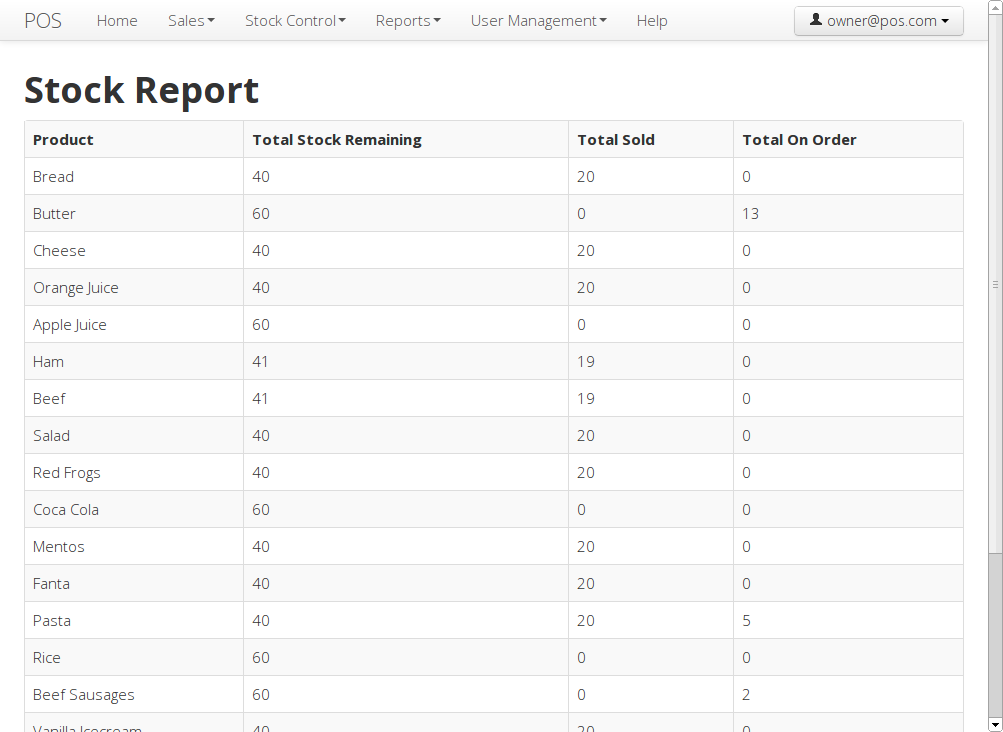
\includegraphics[width=10cm]{d4.png} 
\\\\
\textbf{DN-3.2 The system must have the ability to provide sales reports for management.}
\\\\
This requirement is important as it can shows the performance of the stores/ business using an automated system. This is important because of the complexity of business these days, the system provides great benefit by automatically tracking various types of sales data. The reports produced includes Sales and financial reports. Due to this being a metadata based requirement it was unable to be modelled in event b and hence we had to rely greatly on the requirements description when we were programming for this part of the system. Our financial report also follows standard accounting standards by using a perpetual first in first out approach in managing our inventory costs. The code for the sales and financial report can been seen in the appendix on page 98 and it fulfils the requirement as we requested as seen in the screenshot below: 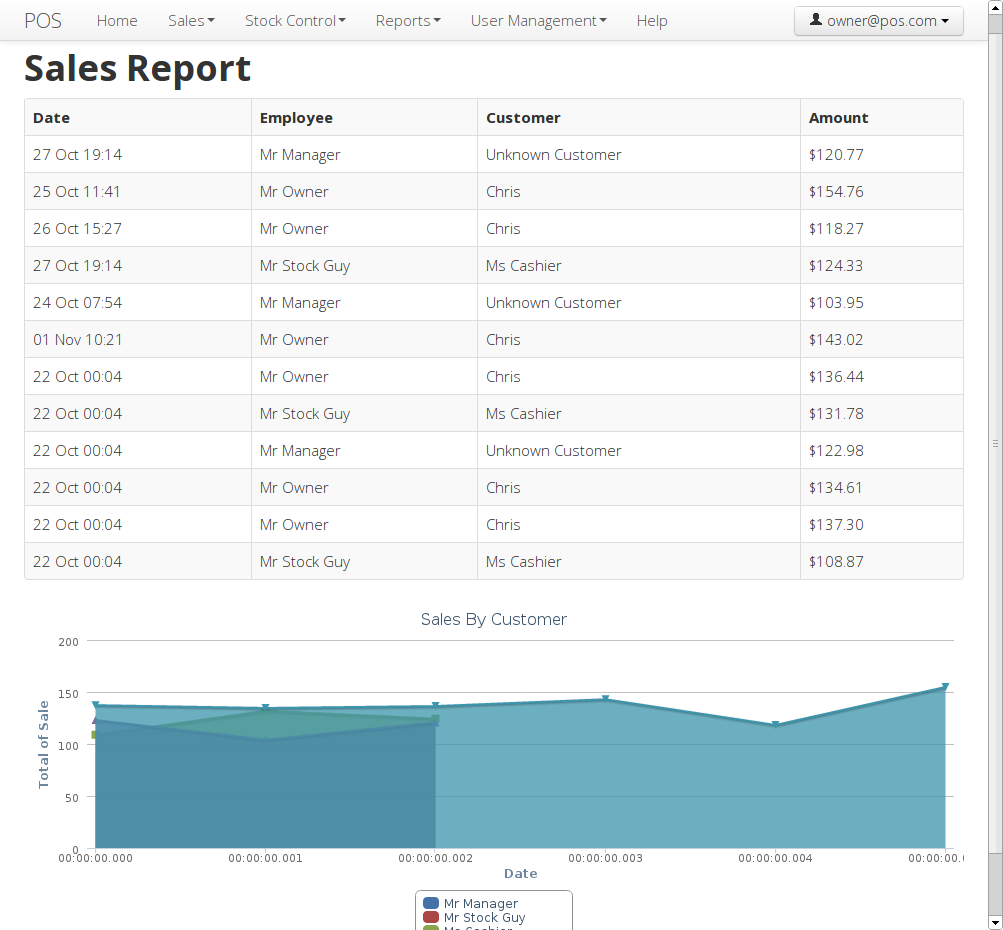
\includegraphics[width=10cm]{d8.png}
\\\\

\textbf{DN-3.3 The system must have the ability to report on system users.}
\\\\
the requirement above as useful in assuring that our system had the ability to track the staff within the system. Due to this being a metadata based requirement it was unable to be modelled in event b and hence we had to rely greatly on the requirements description when we were programming for this part of the system. This mainly consisted of being ability to least the amount and number of sales for each of the system users. The code for this can be seen in the appendix on page 98 and it fulfils the requirement as we requested as seen in the screenshot below. 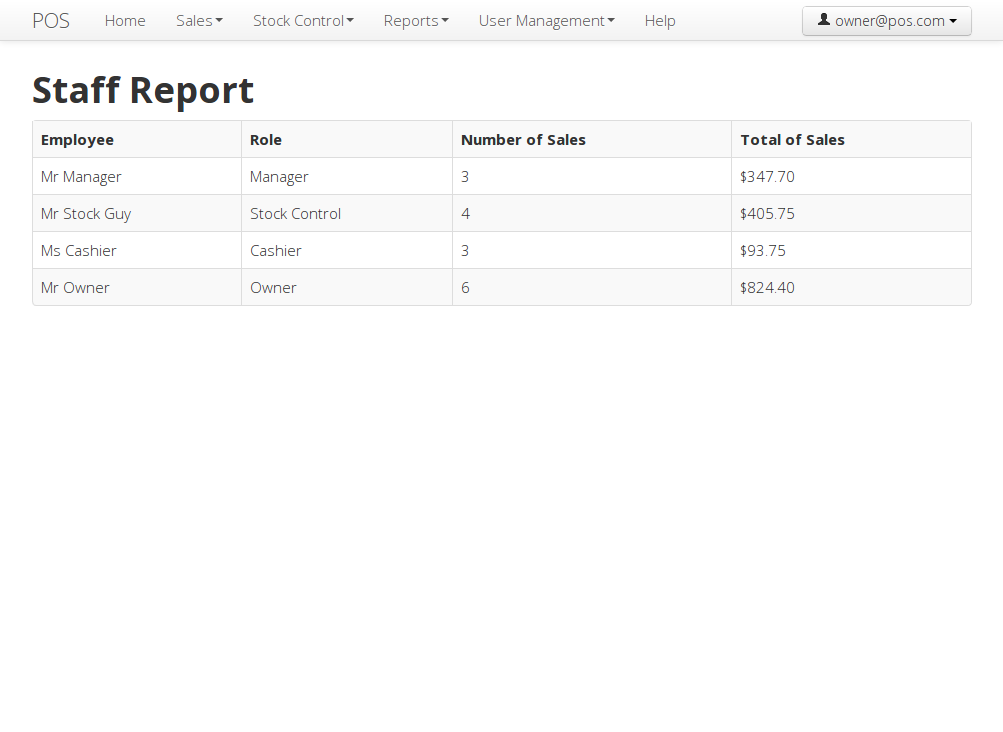
\includegraphics[width=10cm]{d5.png}
\\\\
\textbf{DN-4.1 Support user authentication and multiple levels of authorisation}
\\\\
The user authentication requirement was core to our system ensuring that all the users privacy was maintained as well as ensuring that no one was able to do anything that they couldn't do
\\\\

\section{Design}
The goal of our design was to enable the development of a solution that satisfies the the client’s requirements. This was achiveved in a series of steps, some of which were already outlined in detail in other parts of this document.
\\\\
After a concrete and suitable set of requirements were established, the next most pertinent step verified them for internal consistency. This was vital to the success of the overall project, as it would have been locally impossible to meet two (or more) requirements that were contradictory to each other. If any such contradictions existed, they would surely have been discovered at some stage of the design (or worse, implementation) stage of the project. However by that time, valuable resources could have been wasted developing a partial solution that could not possibly meet all the requirements.
\\\\
Since this is a surprisingly common occurrence in the industry, there are several techniques called formal methods to avoid such a disaster. While there are several to choose from depending on project needs, we used Model Checking. A method of Automated Theorem Proving, with the assistance of EventB’s theorem provers. As such we created a model, that modelled the requirements closely and correctly/accurately as possible within the confines of EventB. This is discussed in detail in the specification section  of this document. While the requirements had to be revised several times during the development of the model, it adequately proved that all parts of the requirements were internally consistent.
\\\\
Since we modelled the requirements so accurately, we were able to proceed from there onwards with little reference to the requirements directly. Due to the lack of natural language, the model was much more suitable to turning directly into a software solution, and as such was the next logical step. 
\\\\
After reexamining the model for this purpose, we determined that it was far to large to be turned into a sustainable software solution. As such, we began decomposing the large monolithic model into a set of smaller, much more manageable components. We displayed such components and the relationships (including dependencies) between them in the somewhat abstract class diagram we presented in our design report. A copy of this is available in appendix(page 24) . 
\\\\
Now that we had our components, their responsibilities and relationships between them, we had to determine the most effective way of turning them into code. This included our choice of paradigm, language, framework and so forth.
\\\\
For ease of development and (more importantly) deployment, we chose to make our solution a ‘web app’. That is,  to have a backend server containing a close implementation of our model, and a front end in a client’s web browser to perform all the inquiry services. Next came the choice of programing language and framework. We opted for ruby on rails, partially due to the advice of our mentors, and because it is a very successful tool in the industry, especially with regards to startups. This is because of the increased developer productivity due to the easy learning curve of Ruby, and the advanced nfoisjure of rails.
\\\\
This essentially meant turning each of those components (or classes, in the class diagram) into an instance of MVC. The models were responsible for dealing with all persistent data (corresponding to variables in the EventB model) in an abstract manner while reals put them to a postgreSQL database. The controllers carried out all the operations on this data, corresponding to events in the EventB model. And the views simply had to present the data in natural format to the user.
\\\\
While we originally intended to design the user interface up front, we decided then that it was best done iteratively, as we built the solution. In a sense we employed a rapid-prototyping approach. For example, the initial interface for checking out a basket involved 3 pages. One for selecting a customer (for record keeping purposes), one for adding products individually, and one for payment. 
\\\\

%%[[screenshot of /sales/new from branch sale_item_2]].
%%[[screenshot of /sales/:id/sale_items from branch sale_item_2]].


It was later decided that it would be tedious to have to make sure the customer was selected before a sale could began as well as having to select a product to add from a list. So this was then redesigned to be a much more streamlined approach, where clicking ‘New Sale’ would take the user directly to the page for scanning products,
%%[[screenshot of /sales/new from master branch ]]$$
\\\\
and the customer (if they were a member) could be selected at a later stage, during payment.

\subsection{Implementation}

Next up, came actually turning the components into a functional solution i.e. ‘writing the code’. During this stage we employed a slightly modified version of the agile approach, implementing on a component by component basis.
\\\
We began by determining the component with the least dependencies such as User, and built it. This involved being able to create, login and edit users. We built this functionality and tested it extensively before proceeding, verifying that it produced the output corresponding exactly to those of the methods in EventB.
We then picked components have no dependencies or depended only on components that are already complete and built them, one at a time. They were also tested rigorously not only to ensure correctness of the overall system, but also to make sure that the components that depend on it won’t have un-explainable bugs. 

\pagebreak
\section{Review and Assessment of prototype implementation}
\pagebreak
\section{Discussion of possible physical deployment}
While designing the point of sale system, we have always kept the idea of physical deployment in mind. As we try to develop a product which will suit the real world needs by utilizing exisiting technology that the world currently offers. 
\\\\
Our point of sales system is made to be easily deployed in various kinds of stores/warehouses. This is due to the ease of setting up and the system’s ability to adapt to a wide range of situations. 
\\\\
For small business the pos system is capable of running on a laptop or even a tablet, with an attaching barcode scanner. While on larger businesses such as supermarkets and warehouses the system can support multiple transaction registers at a time. 
\\\\
The system is also designed to be used with touch input device as the layout of the system is constructed such that buttons and features of the system is well laid out and easily accessible for touch input. 
\\\\
We also had plans during the development stage to include a separate online store for the POS point of sale system. But as we focused more on the core part of the system the online extension was dropped, however it would not take much effort to include such extension as more stores now also offers online purchasing. 
\\\\
Although our system is capable of working with legacy systems, it is highly recommended just to switch over to the new system overall as having both new parts and old parts of the system running concurrently can be problematic. It is also easier to just transfer the historic data over to the new system using the data import method built into the point of sales system. 
\\\\
Our system should also provide frequent updates such that the system can keep up to date with the most advance technology. Updates could be be a built in feature such that the system will automatically check for updates and download + install update components. 
\\\\
A feature which we have implemented in our prototype is the idea of a web based app using cloud computing instead of the classical in store machine and database mix. Firstly this will lead a very fast deployment because instead of installing the software on every single system, clients can just access the application online leading to a faster switch over time between systems. As new stores open they can just connect straight to the application online and the store is up and running. Another great feature about cloud is cheaper maintenance costs as Upgrades are needed less frequently and are typically managed by data centres. This also saves costs in hiring a dedicated IT team each store which contribute to large expenditure for any company. 
\\\\
Overall, the physical deployment of our system will continue to follow one of our core goals: fast, simple and increase efficiency of a business. 
\pagebreak
\section{Assessment of development process}
The development process we took was quite modular it was a long term waterfall development process. the requirements and design stages mainly took place in the previous two semesters. With the implementation and somewhat testing stage taking place this  semester.  Overall the process as a whole functioned correctly and was the most suitable for this time of semi structured and long term project. 
\\\\
In the actual implementation section of the process, we focused on different parts of a system before combining them to work as a whole. This allowed us to easily view our progress, throughout the development period. Generally the process we took worked well it allowed us to create the prototype in a timely manner with minnor issues.
\\\\
As we worked on the different sections we begun most times creating the model  and then adjusting the controller as needed to be able to do all the functions requireed before finally adjusting the views so that there was a usable interface. In some cases when the sections were tightly coupled we were required to work on  both models to gether so that they could be integrated correctly. 
\pagebreak
\section{Project management}
Project management forms a big part of the success or failure of a system design. No matter how great each person in your team is, if the team is unorganised the output of the team will always be unsatisfactory.
\\\\
Hence why it is very important to define a clear scope and goal for our design. As Deming’s 15/85 rule point out, if the first 15"\%" is done correctly, 85"\%" of the desire outcome can achieved. That first drop of water that disturbs the surface of the pool is your first 15"\%". The resulting ripples, right or wrong, all have their origins in that single drop. Our scope and goal was determined since day one and we have set with it ever since.
\\\\
From the requirements design stage to now, we have maintained a proper schedule on the set tasks and the completion date. This was first done using a simple gnatt chart, then we uses a online project management tool mijura, and recently we switched to using another online project management tool - mavenlink. The idea of a project management tool is that it provides tools for scheduling, resource allocation, monitoring and  communication tools between the team members. 
\\\\
Throughout the semesters we have utilized the approach where we get together and discuss what needs to be completed and how to compete such task. The tasks are then posted up on the project management tools online with the due date and comments regarding how we want to achieve the tasks, the tasks are also allocated to the team member(s) elected to complete the tasks. Which we then all all separate and complete the task according to what was defined and within  time allocated to the task. 
\\\\
Communications is also an important aspect in project management. Our teams have various communication channels which we have used. The most common being email, online chats (facebook), online project management tools and video conference (skype, google+). We also have weekly meetings to plan out what each of us are allocated according to the schedule we have set. Meetings and video conferencing is a much prefered communication in our team because of it will require immediate response unlike emails which in some case certain team members would ignore. However, there are rarely times when all team members are free for face to face meeting hence why email remain our main form of contact.
\\\\
 Most of the allocation of tasks are done during the meetings.We bring up the task which is scheduled for the upcoming weeks in the meetings, then the team will discuss what needs to be changed and if there is any tasks which needs priority over others. Our team is particularly good in team work as we often negotiate and have conflict between team member which leads to us not entering into groupthink. Team members also often share new ideas and improvement for the project while voluntarily sharing tasks and responsibilities between team members.
\\\\
Time management is also another important part of project management. As mentioned before with the use of an online project management tool, it minimises the complication of time management and scheduling. Each tasks we have scheduled more than enough time to complete as we understand team members also have other events/ projects they have to attend. However we always require team member to submit their allocated task on time. We have also added padding between our time allocation such that if one person fails to submit a task on time the rest of the team would not get halted since we are missing a component. Mavenlink provides great features such as calendar integration and email reminders close to due date to make sure team members remember the tasks they have to complete. It also makes it easier for project leader as it gives an overview on the tasks which are completed or not completed and to determine if there is a need in the change of scheduling.  Overall our team have worked very well using mavenlink as we rarely have any late night rushing on due dates because of unfinished tasks.
 \\\\
Github was also used throughout the stages to manage our code and ended up being extremely useful as it allowed us all to work simultaneously on the code and we would not have many errors when the code was merged. Also this allows us to revert back changes we made if we found bugs in our system which was very helpful. 
\\\\
During this semester's implementation stage, the way which we used ruby on rails allowed us to split up the work very well with each of us focusing on different modules and later on joining it. This was useful in managing the project as it allowed us to work independently for as long as possible without breaking the whole system. 
\\\\
Overall the combination of tools and decisions during the planning stage allowed us to complete all of the core functionality of the project on time and in the required timeframe. Optimally we would have managed a time a little better and planned more time at the end to add extensions to our projects, as it would have given our project a leading edge. However our project was still done with a very high quality much due to the project management style we utilized since the beginning of project development.

\pagebreak
\section{Special features}
Our project had a variety of different features, that we considered to be special, these were mainly due to our extensions. 
\\\\
One of the key special features in our system was that of the reporting section, the requirement required our system to have a way of providing the managers with a report on different statistics within the system. We decided to add the extra feature of interactive graphs in the sales reports. Which gave our system an easy way to visualise customer sales per customer and as a whole how sales on different dates  to visualise trends. we believe this will be greatly beneficial for users as graphs are a lot easier to understand data than just raw data. 

\begin{figure}[h]
\centering
  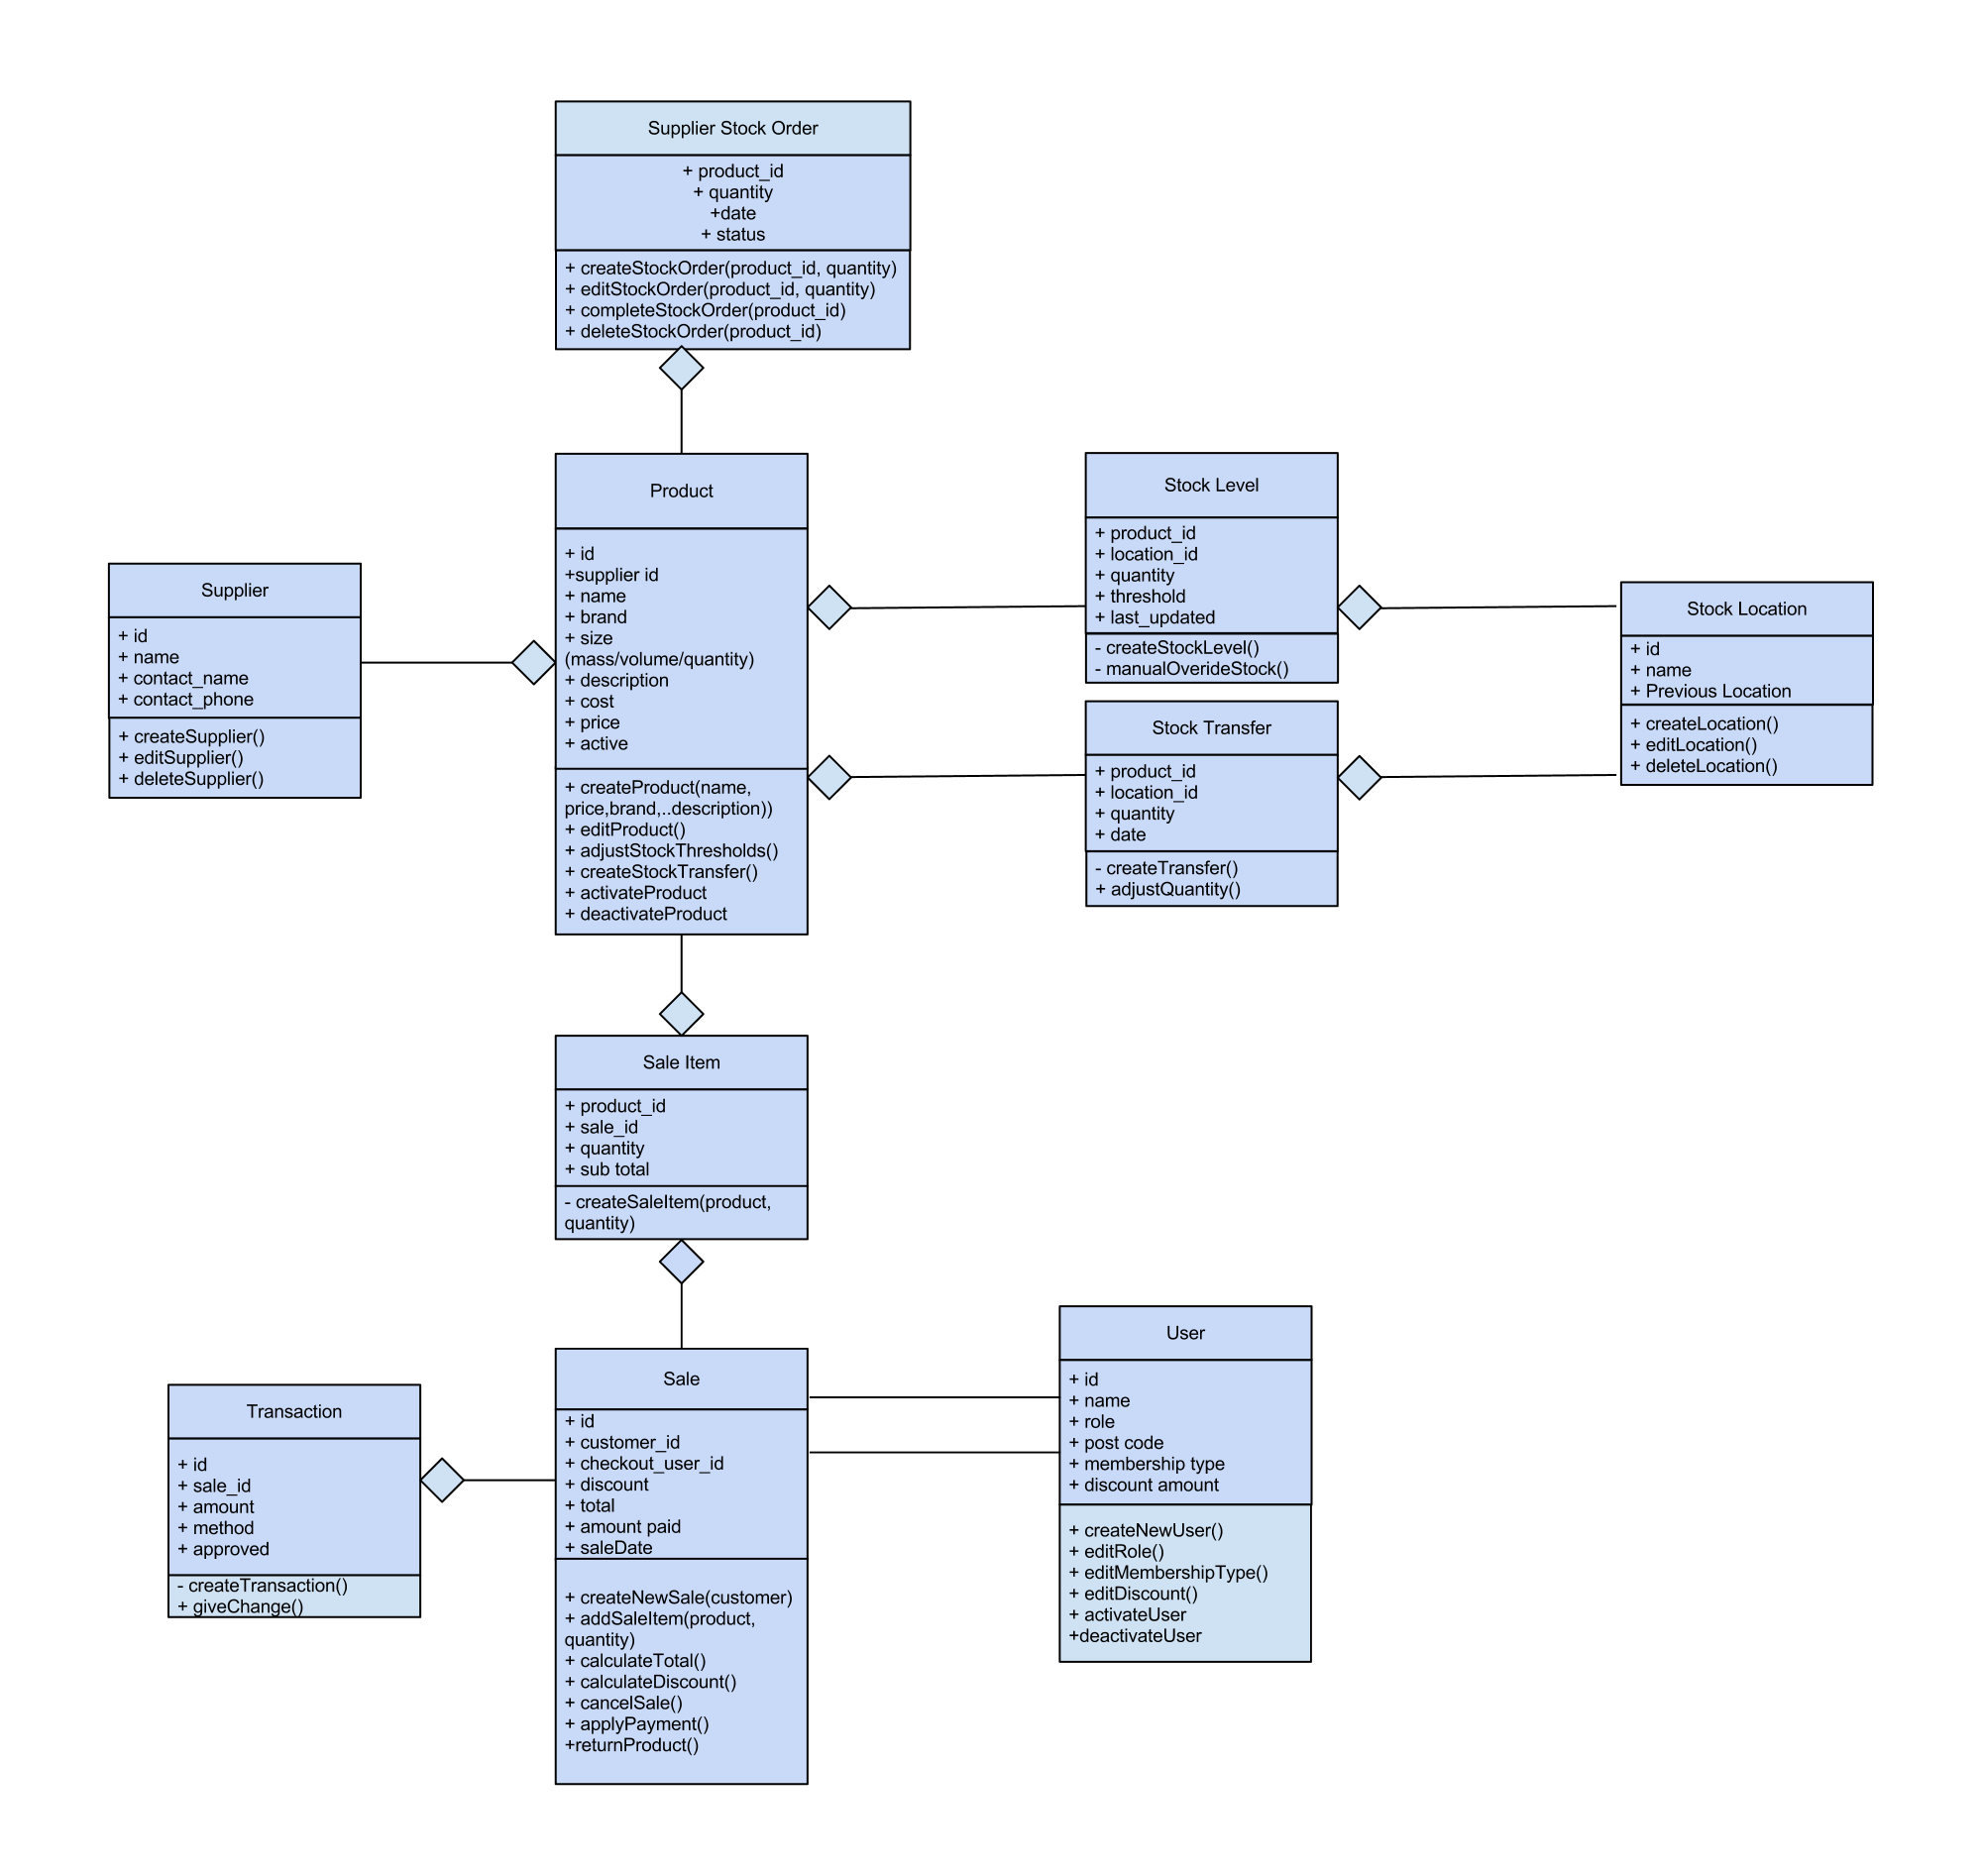
\includegraphics[scale=0.01]{Class diagram.png}
	\caption{Reporting section}
\end{figure}

Another special feature we have included is the way our user interface works. Our system was required to provide a user interface, which was simple and easy to use. We outdone ourselves  with a very simplistic frontend based on the twitter bootstrap. Our user interface also changes according to the current users privileges meaning that what they needed was always less than a click away. This is a particular good feature as the features which are not avliable to the users due to the authorisation status is simply not shown. We have also included a help system was a click away and even though it was not complete it was one of the special features which set our system apart from the other POS developed.


\begin{figure}[h]
\centering
  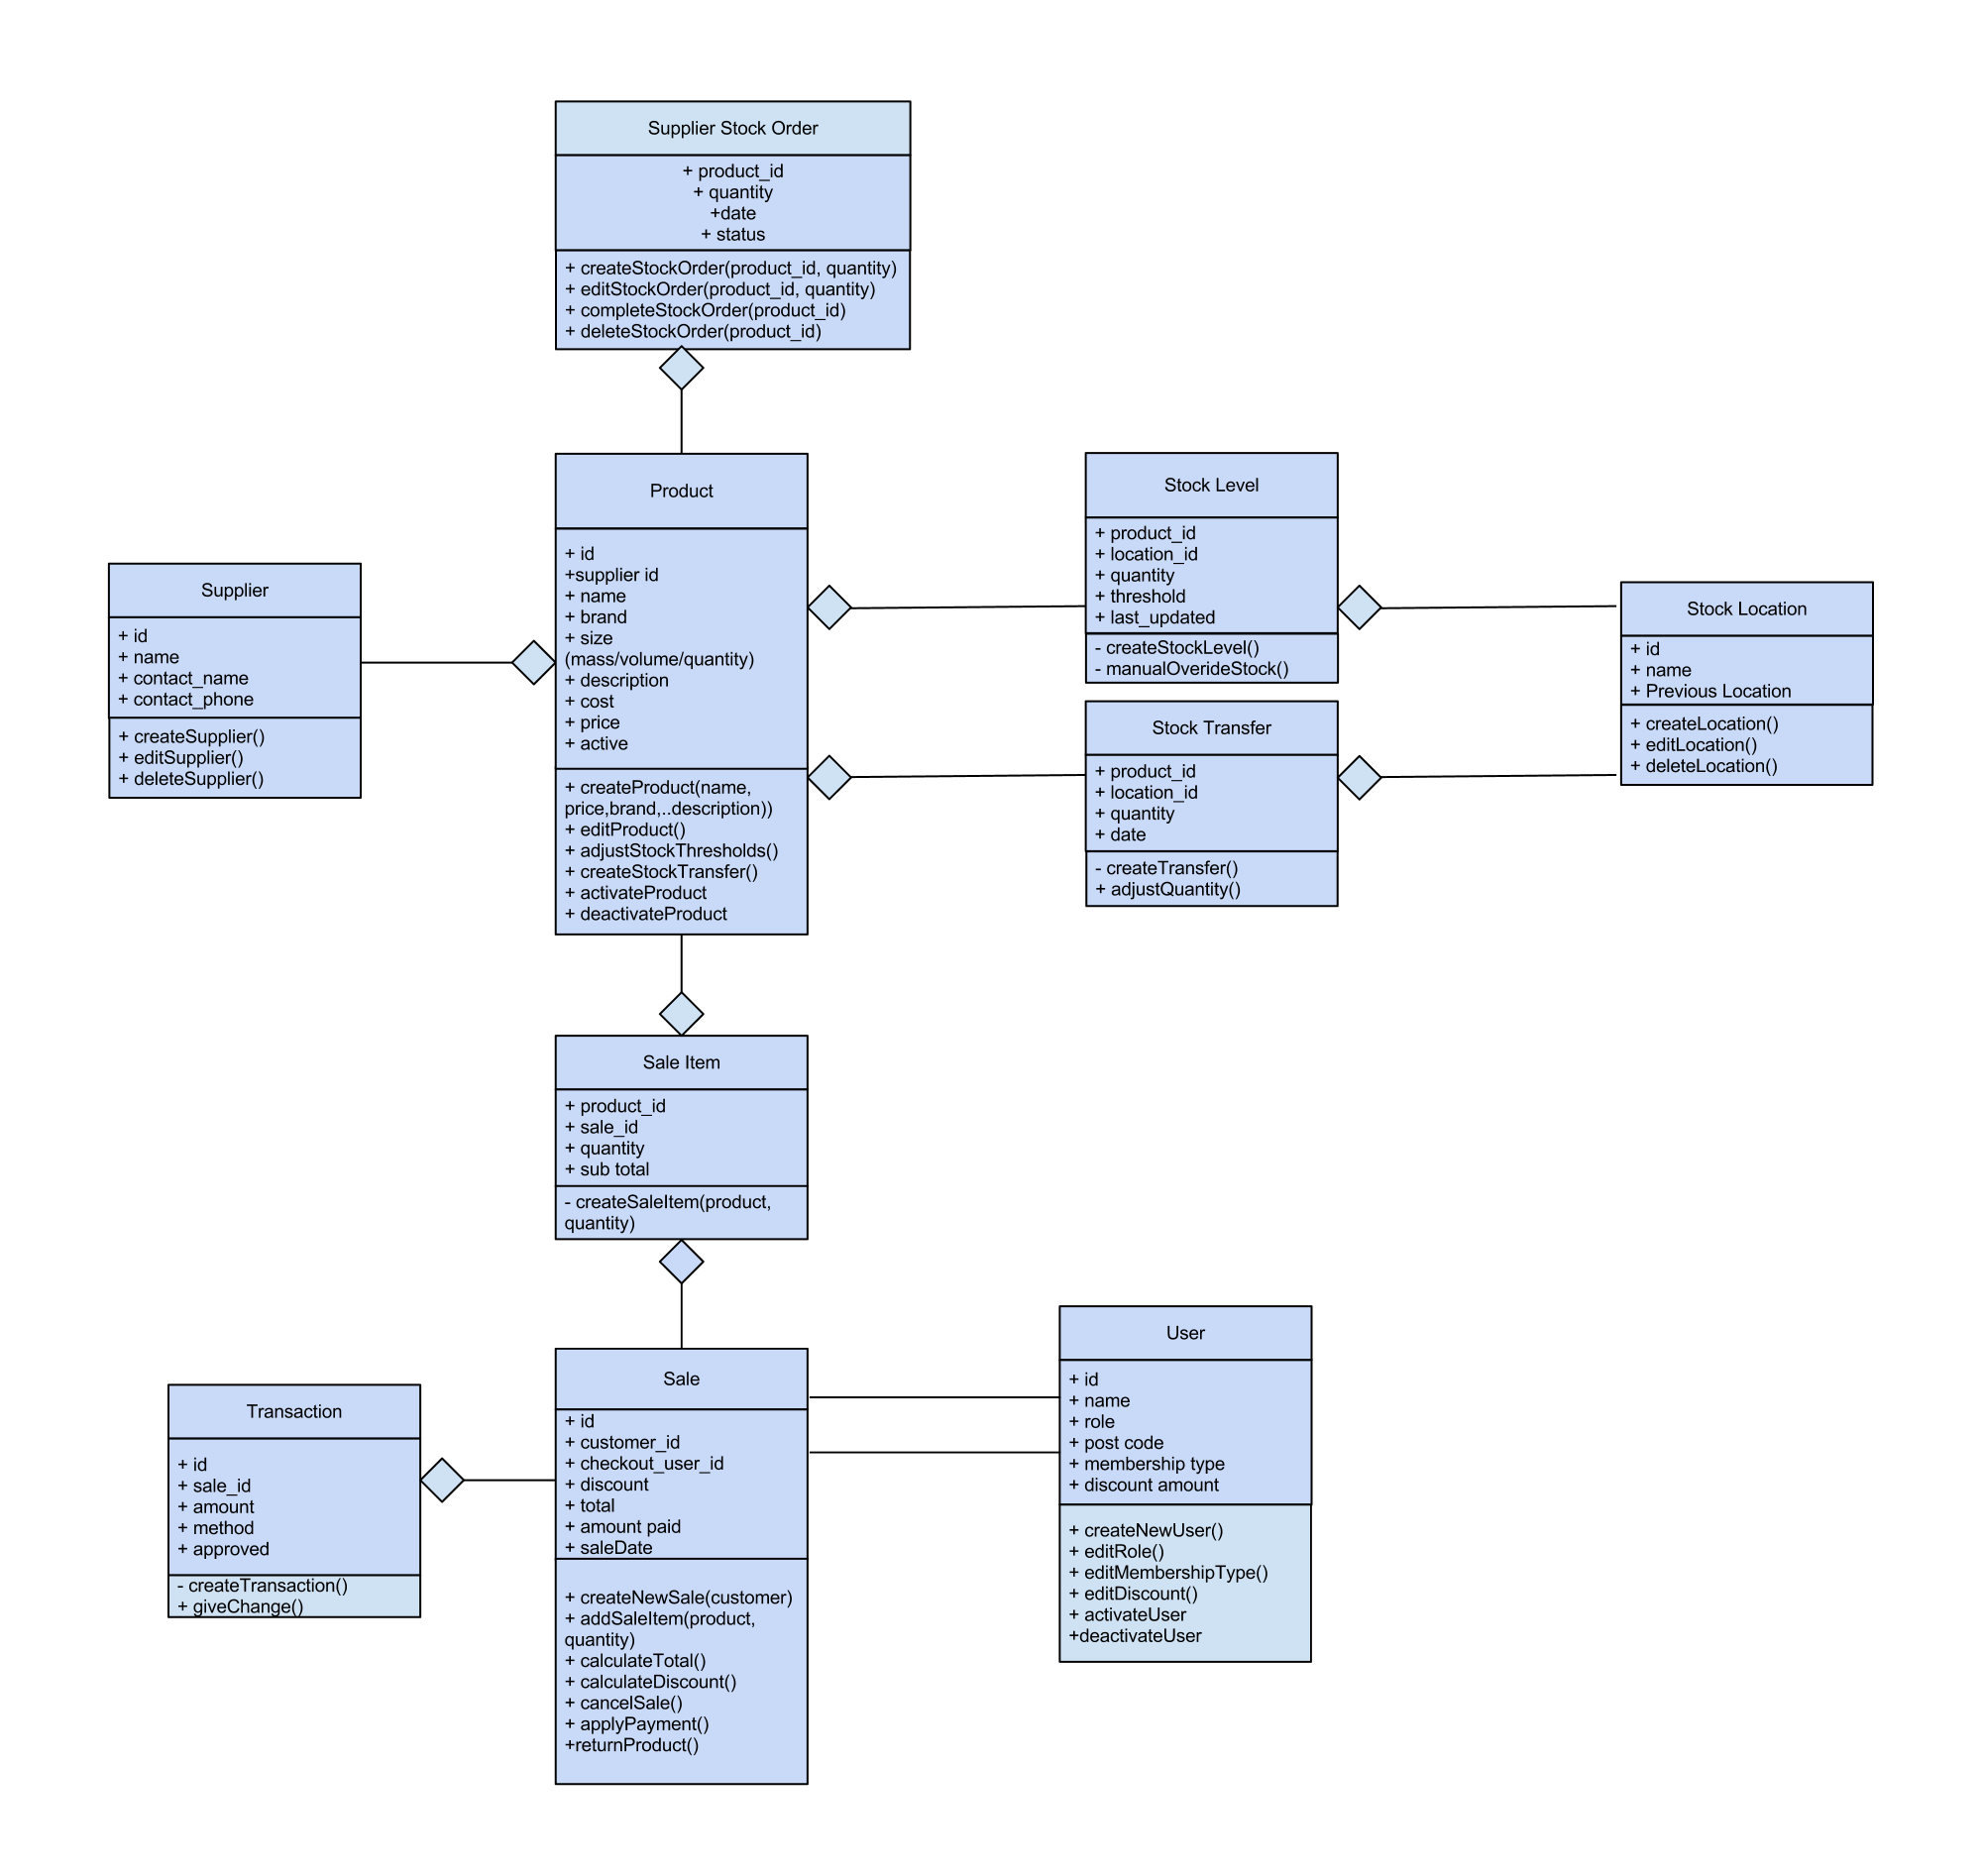
\includegraphics[scale=0.01]{Class diagram.png}
	\caption{User interface}
\end{figure}

Our sales section also features special features which include automatically saving of unfinished transactions. As transactions is only considered complete when its paid for some unforeseen reason the system disconnected, if it then was reconnected it will ask if the user want to continue with their unfinished checkout. Another special features is the overview screen of sales. It shows all the sales currently happening in the store in one page. It categorise by if products are being scanned, they are checking out or completed. This way the store wont get hold up by customers as it can just save their transaction and serve the next customer before going back to the original customer (for example if a customer wants price check)  
 
\pagebreak

\section{Reflections and Introspection}


Although our project ran quite smoothly there were a few areas which we think we could improve on, firstly being the implementation of extra features. As we did schedule a time for our extensions but we had a lot more extensions than we initially thought we had. Extensions which are not implemented yet includes qr code scanning, product details importation and online stores. I believe we could have changed our timetable such that we have sufficient time to finish all the set extensions.
\\\\
We also could have tried to improve on our code, most it worked however there are patches from quick fixes which are not the best way of implementation. There are also some areas which have bugs and we didn't have time to fix. This is again due to poor time allocation between different tasks as testing took up a lot more time than we initially thought it would take. 
\\\\
If we could have spent more on the project we could have found a solution to see if we could simultaneously edit the database without any overwrite issues. We had a few ideas during the implementation however most of them we either don't know or were too complex to implement into our system. 
\\\\
A definite problem we have in this project is the lack of communication between team members, as team members does not reply to email at times and wanting to do parts which they are not assigned. This leads to overwriting of codes where one person finish a section, and another person just came in with their own version and overwrites everything the last person wrote. A way to improve this will be better communications between team members as the team members can both work together on the same section for the best outcome.
\\\\
Another improvement we could have made is by testing with 3rd party, for example our payment system so far just assumes the card transaction is always approved, however we could have tested with 3rd party applications to see the various kinds of interaction and if there are any areas which becomes problematic. 
\\\\
On the whole, the code was done with a high standard, though we could have improved in some areas by not  relying on the scaffolding as much as we did, but given the short time frame we had this was probably the best solution. 
\\\\
At times we also strayed away from our requirements, as we found new ways and ideas for our system. This could have improved by creating a better set of requirements at the beginning as it is clear we haven't thought of everything, but also could have been improved if we constantly made comparisons of our current solution with the requirements to make sure we our code is compliant to what we set out. This is an indication of the importance of design as our initial design werent the best, which leads to our project being problematic during implementation. Although we still manage to solve the problems we had, it will be much easier if we have had a better design at the beginning. 
\\\\
Overall, I think we did well as a team. Our implementation works and we also implemented a few extra features. Although there are still a few bugs in our system and our team had minor problems at times, we did well as a team overall. As teams without conflicts are not an efficient team and conflict is a natural result of teamwork.  All of us learnt a lot regarding design as we finally see the importance of both the requirements and event-b modelling during the implementation stage. 
\pagebreak


\section{Appendix}

\subsection{Class Diagram}

\begin{figure}[h]
\centering
  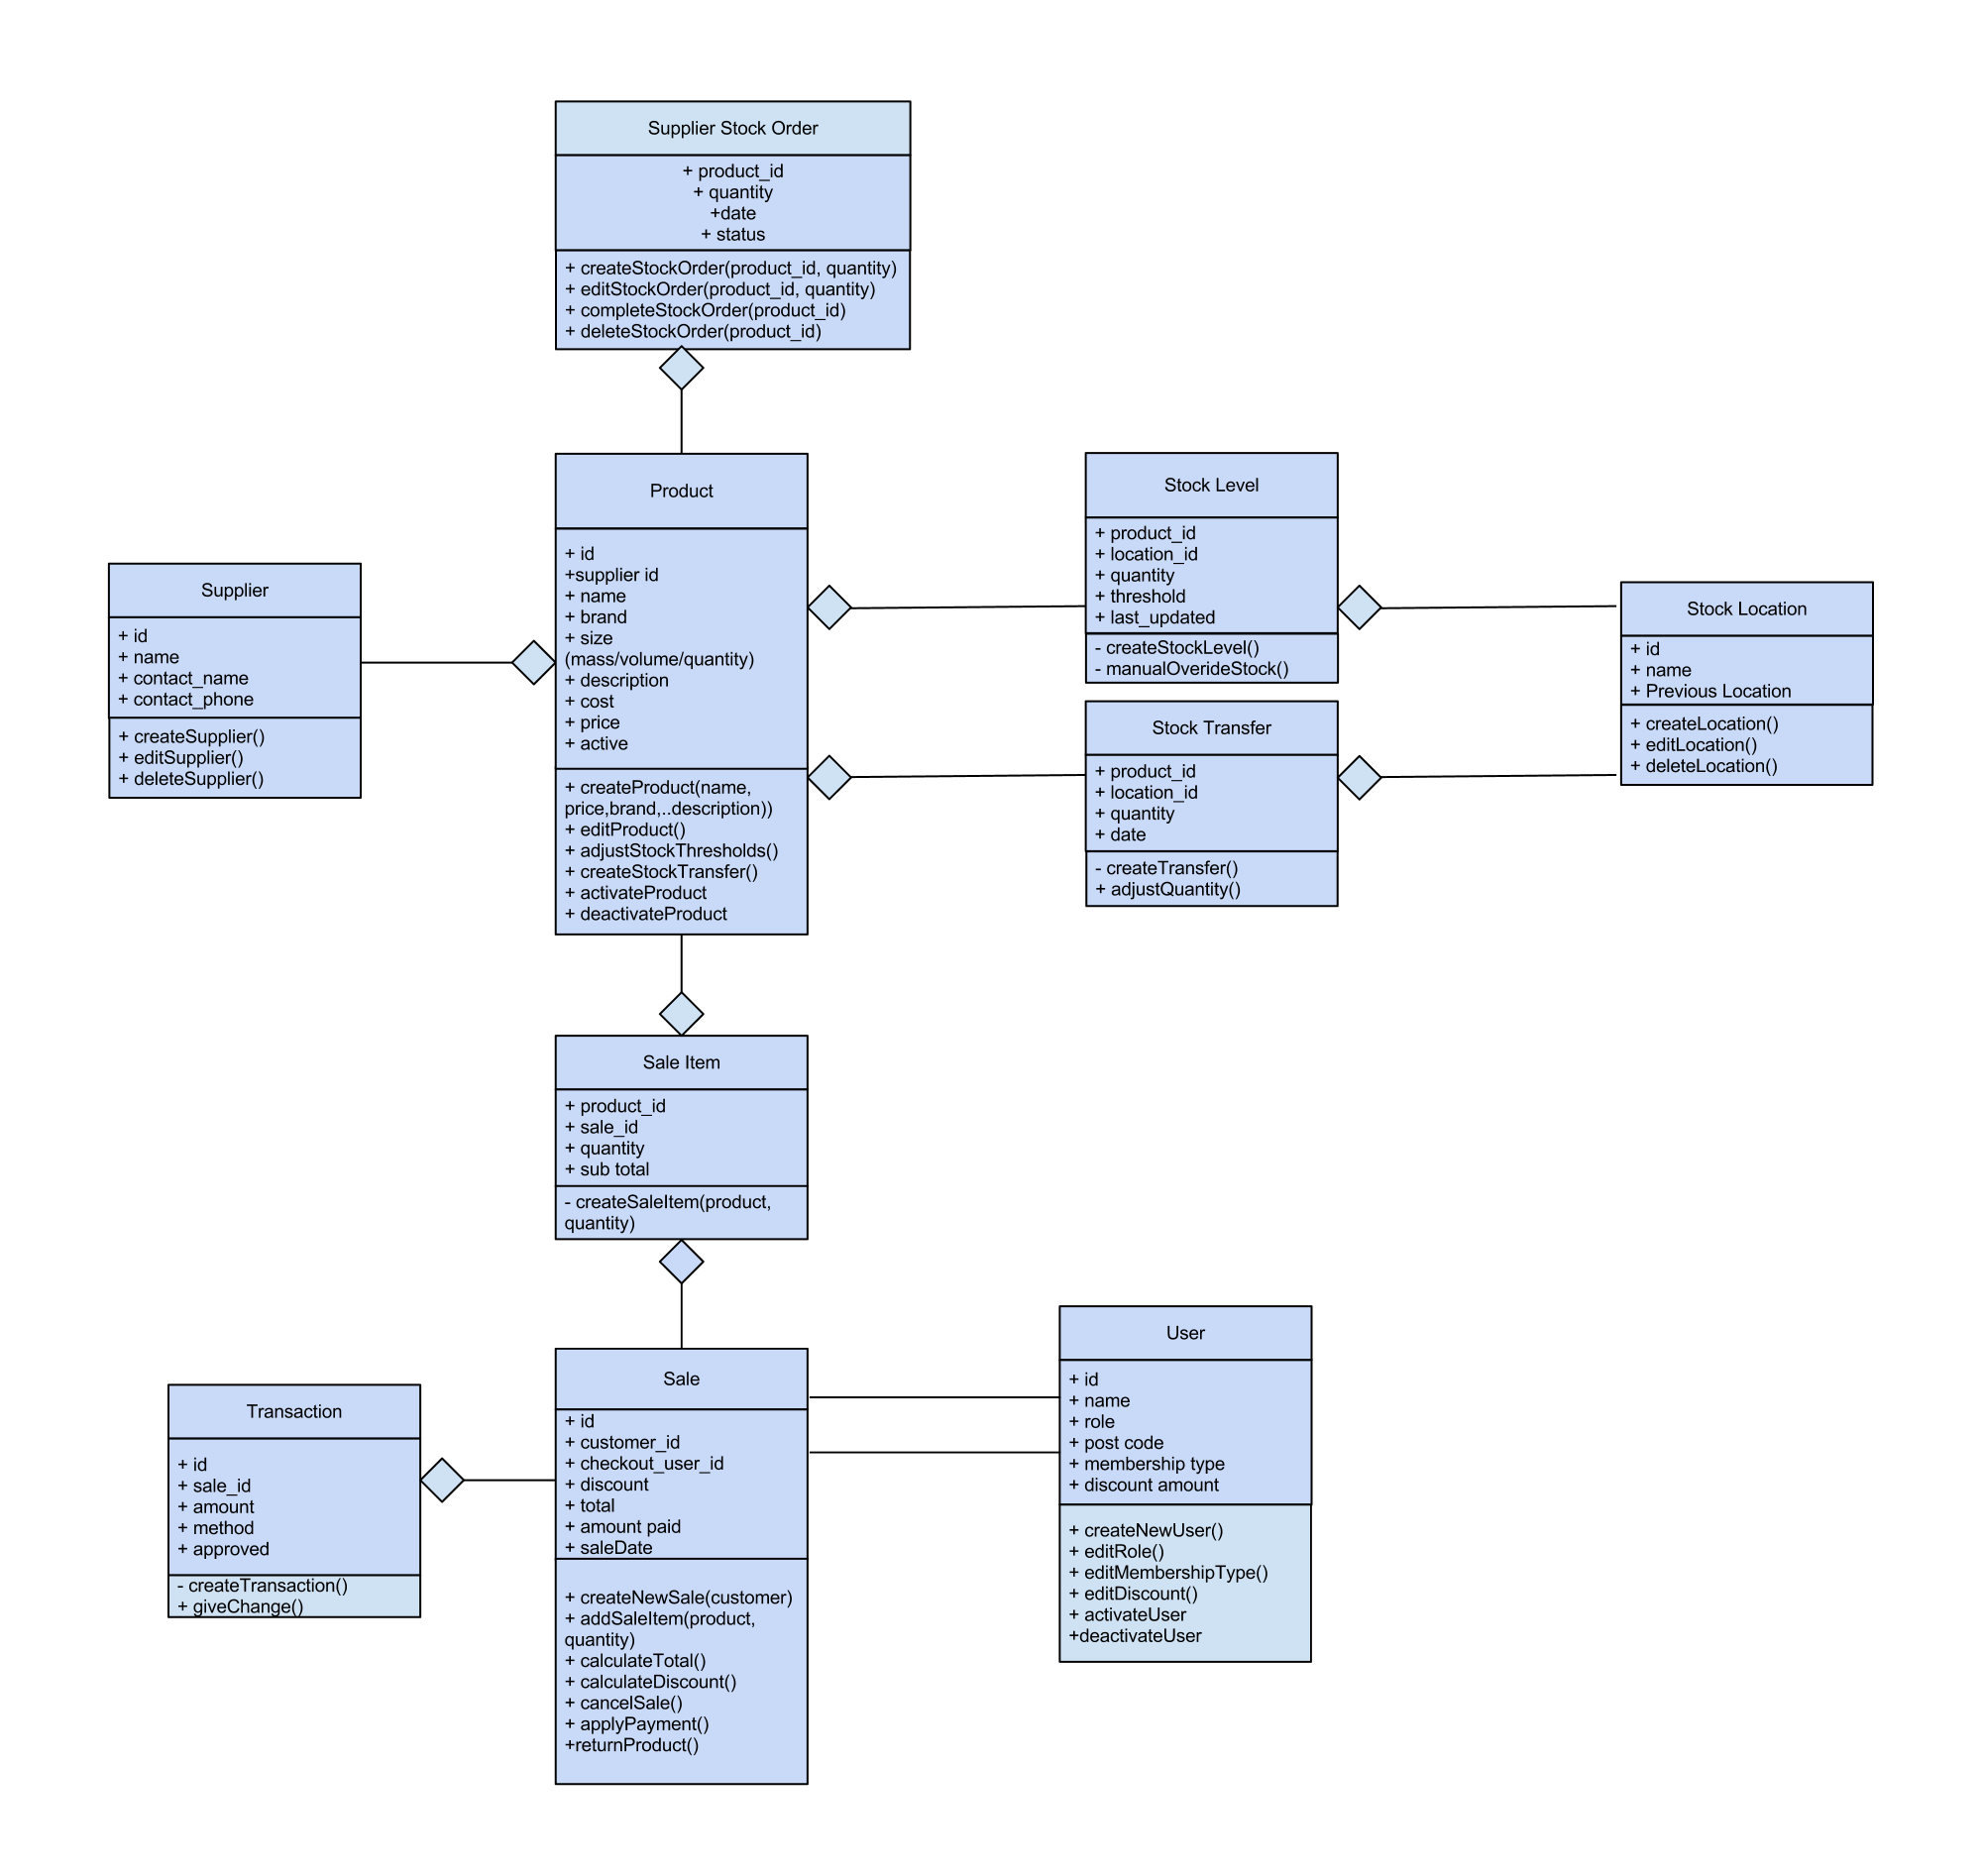
\includegraphics[scale=0.2]{Class diagram.png}
	\caption{Class Diagram for our POS system}
\end{figure}

\pagebreak
\subsection{Event-B Model}

%% Note
% It is possible to interleave the model with the discussion
% To do this the LaTeX-ed Event-B models would need to be
% broken into pieces.  Each piece should be inside a

% \begin{description}
% \MACHINE{myConstruct}
% ...
% \END
% \end{description}

% For more details/instructions please read:
%    eventB-markup.pdf

% You can insert page breaks at points in the machine/context by
% inserting \clearpage commands.

\begin{description}
\subsubsection{Stock\_ctx}
\CONTEXT{Stock\_ctx}
\cmt{ Defines a product and stock location }
\SETS
	\begin{description}
		\Item{ PRODUCT }
		\Item{ STOCK\_LOCATION }
	\end{description}
\CONSTANTS
	\begin{description}
		\Item{ Floor }
		\Item{ Backroom }
		\Item{ Warehouse }
		\Item{ thresholdmax }
	\end{description}
\AXIOMS
	\begin{description}
		\nItemX{ axm1 }{ finite(PRODUCT) }
		\nItemX{ axm2 }{ partition(STOCK\_LOCATION,\{ Floor\} ,\{ Backroom\} ,\{ Warehouse\} ) }
		\nItemX{ axm3 }{ thresholdmax\in \nat }
	\end{description}
\END
\end{description}

\begin{description}
\subsubsection{Stock\_ctx\_R0}
\CONTEXT{Stock\_ctx\_R0}
\cmt{ Defines users and userprivileges }
\EXTENDS{Stock\_ctx}
\SETS
	\begin{description}
		\Item{ USERS }
		\Item{ USER\_PRIVILEGE }
	\end{description}
\CONSTANTS
	\begin{description}
		\Item{ Cashier }
		\Item{ Stock\_Control }
		\Item{ Manager }
		\Item{ Owner }
	\end{description}
\AXIOMS
	\begin{description}
		\nItemX{ axm1 }{ finite(USERS) }
		\nItemX{ axm2 }{ partition(USER\_PRIVILEGE,\{ Cashier\} ,\{ Stock\_Control\} ,\{ Manager\} ,\{ Owner\} ) }
		\cmt{ PD-4.1.2 - Provide various levels of access control to the system. }
	\end{description}
\END
\end{description}

\begin{description}
\pagebreak
\subsubsection{Stock\_ctx\_R1}
\CONTEXT{Stock\_ctx\_R1}
\EXTENDS{Stock\_ctx\_R0}
\SETS
	\begin{description}
		\Item{ ORDER\_STATUS }
	\end{description}
\CONSTANTS
	\begin{description}
		\Item{ Created }
		\Item{ Completed }
		\Item{ Delivering }
	\end{description}
\AXIOMS
	\begin{description}
		\nItemX{ axm1 }{ partition(ORDER\_STATUS, \{ Created\} ,\{ Delivering\} ,\{ Completed\} ) }
	\end{description}
\END
\end{description}

\begin{description}
\subsubsection{Stock\_ctx\_R2}
\CONTEXT{Stock\_ctx\_R2}
\EXTENDS{Stock\_ctx\_R1}
\SETS
	\begin{description}
		\Item{ MEMBERS }
		\Item{ TRANSACTIONTYPE }
	\end{description}
\CONSTANTS
	\begin{description}
		\Item{ CART }
		\Item{ emptycart }
		\Item{ ADDINGTOCART }
		\Item{ CHECKINGOUT }
		\Item{ FINISHED }
	\end{description}
\AXIOMS
	\begin{description}
		\nItemX{ axm1 }{ CART = PRODUCT \pfun  \nat }
		\nItemX{ axm2 }{ emptycart = PRODUCT \cprod  \{ 0\}  }
		\nItemX{ axm3 }{ partition(TRANSACTIONTYPE, \{ ADDINGTOCART\} ,\{ CHECKINGOUT\} ,\{ FINISHED\} ) }
	\end{description}
\END
\end{description}

\begin{description}
\pagebreak
\subsubsection{StockControl}
\MACHINE{StockControl}
\cmt{ DN-1.1 - The base machine focuses on the systems ability to provide the capability to modify the current stock data. }
\SEES{Stock\_ctx}
\VARIABLES
	\begin{description}
		\Item{ products }
		\bcmt{ the set of all products in the system }
		\Item{ productprice }
		\bcmt{ the set of all product prices }
		\Item{ productthreshold }
		\bcmt{ the set of all product thresholds }
		\Item{ productlevels }
		\bcmt{ the set of all product levels }
		\Item{ activeProducts }
		\bcmt{ the set of currently activated products }
	\end{description}
\INVARIANTS
	\begin{description}
		\nItemX{ inv1 }{ products \subseteq  PRODUCT }
		\nItemX{ inv2 }{ productprice \in  products \tfun  \nat }
		\nItemX{ inv5 }{ productthreshold \in  products \tfun  (STOCK\_LOCATION \tfun  \nat) }
		\nItemX{ inv7 }{ productlevels \in  products \tfun (STOCK\_LOCATION \tfun  \nat) }
		\nItemX{ inv8 }{ activeProducts \subseteq  products }
		\nItemX{ inv9 }{ \forall p,l \qdot  p\in  activeProducts \land  l \in  STOCK\_LOCATION \limp  productlevels(p)(l) \geq  productthreshold(p)(l) }
		\nItemX{ inv10 }{ \forall p,l \qdot  p\in  products\setminus activeProducts \land  l \in  STOCK\_LOCATION \limp  productlevels(p)(l) = 0 }
		\nItemX{ inv11 }{ finite(products) }
		\nItemX{ inv12 }{ finite(activeProducts) }
		\nItemX{ inv13 }{ \forall p,l \qdot  p\in  products \land  l \in  STOCK\_LOCATION \limp  productlevels(p)(l) \in \nat }
		\nItemX{ inv14 }{ \forall p,l \qdot  p\in  products \land  l \in  STOCK\_LOCATION \limp  productthreshold(p)(l) \in \nat }
	\end{description}
\EVENTS
	\INITIALISATION
		\begin{description}
		\BeginAct
			\begin{description}
			\nItemX{ act1 }{ products :=  \emptyset  }
			\nItemX{ act2 }{ productprice :=  \emptyset  }
			\nItemX{ act3 }{ productthreshold :=  \emptyset  }
			\cmt{ individual product thresholds }
			\nItemX{ act4 }{ productlevels :=  \emptyset  }
			\cmt{ individual product levels }
			\nItemX{ act5 }{ activeProducts :=  \emptyset  }
			\end{description}
		\EndAct
		\end{description}
	\EVT {NewProduct}
	\cmt{ PD-1.1.2 Add new product to the database }
		\begin{description}
		\AnyPrm
			\begin{description}
			\ItemX{ product }
			\ItemX{ price }
			\end{description}
		\WhereGrd
			\begin{description}
			\nItemX{ grd1 }{ product \in  PRODUCT\setminus products }
			\nItemX{ grd2 }{ price \in  \nat }
			\nItemX{ grd3 }{ product \notin  activeProducts }
			\nItemX{ grd4 }{ product \notin  products }
			\end{description}
		\ThenAct
			\begin{description}
			\nItemX{ act1 }{ products :=  products \bunion  \{ product\}  }
			\nItemX{ act2 }{ productprice(product) :=  price }
			\nItemX{ act4 }{ productthreshold(product) :=  STOCK\_LOCATION \cprod  \{ 0\}  }
			\nItemX{ act5 }{ productlevels(product) :=  STOCK\_LOCATION \cprod  \{ 0\}  }
			\end{description}
		\EndAct
		\end{description}
	\EVT {UpdateProduct}
	\cmt{ PD-1.1.3 Update a products details }
		\begin{description}
		\AnyPrm
			\begin{description}
			\ItemX{ product }
			\ItemX{ price }
			\end{description}
		\WhereGrd
			\begin{description}
			\nItemX{ grd1 }{ product \in  products }
			\nItemX{ grd2 }{ price \in  \nat }
			\end{description}
		\ThenAct
			\begin{description}
			\nItemX{ act1 }{ productprice(product) :=  price }
			\end{description}
		\EndAct
		\end{description}
	\EVT {SetProductThreshold}
	\cmt{ PD-1.4.4 Allow stock level thresholds to be set }
		\begin{description}
		\AnyPrm
			\begin{description}
			\ItemX{ product }
			\ItemX{ floor }
			\ItemX{ backroom }
			\ItemX{ warehouse }
			\end{description}
		\WhereGrd
			\begin{description}
			\nItemX{ grd1 }{ product \in  activeProducts }
			\nItemX{ grd2 }{ floor \in  1\upto productlevels(product)(Floor) }
			\nItemX{ grd3 }{ backroom \in  1\upto productlevels(product)(Backroom) }
			\nItemX{ grd4 }{ warehouse \in  1\upto productlevels(product)(Warehouse) }
			\nItemX{ grd5 }{ productlevels(product)(Floor) \geq  floor }
			\nItemX{ grd6 }{ productlevels(product)(Backroom) \geq  backroom }
			\nItemX{ grd7 }{ productlevels(product)(Warehouse) \geq  warehouse }
			\end{description}
		\ThenAct
			\begin{description}
			\nItemX{ act1 }{ productthreshold(product) :=  \{ Floor \mapsto  floor,Backroom \mapsto  backroom,Warehouse \mapsto  warehouse\}  }
			\end{description}
		\EndAct
		\end{description}
	\EVT {SetProductLevel}
		\begin{description}
		\AnyPrm
			\begin{description}
			\ItemX{ product }
			\ItemX{ floor }
			\ItemX{ backroom }
			\ItemX{ warehouse }
			\end{description}
		\WhereGrd
			\begin{description}
			\nItemX{ grd1 }{ product \in  activeProducts }
			\nItemX{ grd2 }{ floor \in  productthreshold(product)(Floor)\upto thresholdmax }
			\nItemX{ grd3 }{ backroom \in  productthreshold(product)(Backroom)\upto thresholdmax }
			\nItemX{ grd4 }{ warehouse \in  productthreshold(product)(Warehouse)\upto thresholdmax }
			\nItemX{ grd5 }{ floor \geq  productthreshold(product)(Floor) }
			\nItemX{ grd6 }{ backroom \geq  productthreshold(product)(Backroom) }
			\nItemX{ grd7 }{ warehouse \geq  productthreshold(product)(Warehouse) }
			\end{description}
		\ThenAct
			\begin{description}
			\nItemX{ act1 }{ productlevels(product) :=  \{ Floor \mapsto  floor,Backroom \mapsto  backroom,Warehouse \mapsto  warehouse\}  }
			\end{description}
		\EndAct
		\end{description}
	\EVT {MoveStockToFloor}
	\cmt{ PD-1.4.2 Ability to request stock from other locations }
		\begin{description}
		\AnyPrm
			\begin{description}
			\ItemX{ amount }
			\ItemX{ product }
			\end{description}
		\WhereGrd
			\begin{description}
			\nItemX{ grd2 }{ product \in  activeProducts }
			\nItemX{ grd1 }{ amount \in  1\upto (productlevels(product)(Backroom) -  productthreshold(product)(Backroom)) }
			\nItemX{ grd3 }{ productlevels(product)(Backroom) \geq  productthreshold(product)(Backroom) + amount }
			\nItemX{ grd4 }{ productlevels(product)(Floor) \geq  productthreshold(product)(Floor) }
			\end{description}
		\ThenAct
			\begin{description}
			\nItemX{ act1 }{ productlevels(product) :=  productlevels(product) \ovl  \{ Floor \mapsto  (productlevels(product)(Floor) + amount),Backroom \mapsto  (productlevels(product)(Backroom) -  amount)\}  }
			\end{description}
		\EndAct
		\end{description}
	\EVT {MoveStockToBackroom}
	\cmt{ PD-1.4.2 Ability to request stock from other locations }
		\begin{description}
		\AnyPrm
			\begin{description}
			\ItemX{ amount }
			\ItemX{ product }
			\end{description}
		\WhereGrd
			\begin{description}
			\nItemX{ grd2 }{ product \in  activeProducts }
			\nItemX{ grd1 }{ amount \in  1\upto (productlevels(product)(Warehouse) -  productthreshold(product)(Warehouse)) }
			\nItemX{ grd3 }{ productlevels(product)(Warehouse) \geq  productthreshold(product)(Warehouse) + amount }
			\nItemX{ grd4 }{ productlevels(product)(Backroom) \geq  productthreshold(product)(Backroom) }
			\end{description}
		\ThenAct
			\begin{description}
			\nItemX{ act1 }{ productlevels(product) :=  productlevels(product) \ovl  \{ Backroom \mapsto  (productlevels(product)(Backroom) + amount),Warehouse \mapsto  (productlevels(product)(Warehouse) -  amount)\}  }
			\end{description}
		\EndAct
		\end{description}
	\EVT {RemoveStock}
	\cmt{ PD 1.1.1 Ability to add/remove stock from a location. }
		\begin{description}
		\AnyPrm
			\begin{description}
			\ItemX{ product }
			\ItemX{ amount }
			\ItemX{ location }
			\end{description}
		\WhereGrd
			\begin{description}
			\nItemX{ grd1 }{ product \in  activeProducts }
			\nItemX{ grd2 }{ amount \in  1\upto (productlevels(product)(location) -  productthreshold(product)(location)) }
			\nItemX{ grd3 }{ location \in  STOCK\_LOCATION }
			\nItemX{ grd4 }{ productlevels(product)(location) \geq  productthreshold(product)(location) + amount }
			\end{description}
		\ThenAct
			\begin{description}
			\nItemX{ act1 }{ productlevels(product) :=  productlevels(product) \ovl  \{ location \mapsto  (productlevels(product)(location) -  amount)\}  }
			\end{description}
		\EndAct
		\end{description}
	\EVT {AddStock}
	\cmt{ PD 1.1.1 Ability to add/remove stock from a location. }
		\begin{description}
		\AnyPrm
			\begin{description}
			\ItemX{ product }
			\ItemX{ amount }
			\ItemX{ location }
			\end{description}
		\WhereGrd
			\begin{description}
			\nItemX{ grd1 }{ product \in  activeProducts }
			\nItemX{ grd2 }{ amount \in  \nat_1 }
			\nItemX{ grd3 }{ location \in  STOCK\_LOCATION }
			\end{description}
		\ThenAct
			\begin{description}
			\nItemX{ act1 }{ productlevels(product) :=  productlevels(product) \ovl  \{ location \mapsto  (productlevels(product)(location) + amount)\}  }
			\end{description}
		\EndAct
		\end{description}
	\EVT {ActivateProduct}
		\begin{description}
		\AnyPrm
			\begin{description}
			\ItemX{ product }
			\end{description}
		\WhereGrd
			\begin{description}
			\nItemX{ grd1 }{ product \in  products }
			\nItemX{ grd2 }{ product \notin  activeProducts }
			\end{description}
		\ThenAct
			\begin{description}
			\nItemX{ act1 }{ activeProducts :=  activeProducts \bunion  \{ product\}  }
			\nItemX{ act2 }{ productlevels(product) :=  STOCK\_LOCATION \cprod  \{ 0\}  }
			\nItemX{ act3 }{ productthreshold(product) :=  STOCK\_LOCATION \cprod  \{ 0\}  }
			\end{description}
		\EndAct
		\end{description}
	\EVT {DeactivateProduct}
	\cmt{ PD-1.1.4 Remove a product from the system }
		\begin{description}
		\AnyPrm
			\begin{description}
			\ItemX{ product }
			\end{description}
		\WhereGrd
			\begin{description}
			\nItemX{ grd1 }{ product \in  activeProducts }
			\nItemX{ grd2 }{ product \in  products }
			\end{description}
		\ThenAct
			\begin{description}
			\nItemX{ act1 }{ activeProducts :=  activeProducts\setminus \{ product\}  }
			\nItemX{ act2 }{ productlevels(product) :=  STOCK\_LOCATION \cprod  \{ 0\}  }
			\end{description}
		\EndAct
		\end{description}
\END
\end{description}

\begin{description}
\pagebreak
\subsubsection{StockControl\_R0}
\MACHINE{StockControl\_R0}
\cmt{ DN-4.1 - This refinement is concerned with user authentication and multiple levels of authorisation }
\REFINES{StockControl}
\SEES{Stock\_ctx\_R0}
\VARIABLES
	\begin{description}
		\Item{ products }
		\Item{ productprice }
		\Item{ productthreshold }
		\Item{ productlevels }
		\Item{ activeProducts }
		\Item{ users }
		\Item{ userPrivileges }
	\end{description}
\INVARIANTS
	\begin{description}
		\nItemX{ inv1 }{ users \subseteq  USERS }
		\nItemX{ inv2 }{ userPrivileges \in  users \tfun  USER\_PRIVILEGE }
	\end{description}
\EVENTS
	\INITIALISATION
		\\\textit{extended}
		\begin{description}
		\BeginAct
			\begin{description}
			\nItem{ act1 }{ products :=  \emptyset  }
			\nItem{ act2 }{ productprice :=  \emptyset  }
			\nItem{ act3 }{ productthreshold :=  \emptyset  }
			\cmt{ individual product thresholds }
			\nItem{ act4 }{ productlevels :=  \emptyset  }
			\cmt{ individual product levels }
			\nItem{ act5 }{ activeProducts :=  \emptyset  }
			\nItemX{ act6 }{ users :=  \emptyset  }
			\nItemX{ act7 }{ userPrivileges :=  \emptyset  }
			\end{description}
		\EndAct
		\end{description}
	\EVT {NewUser}
	\cmt{ PD-4.1.1 - Provide User Authentication \& PD-4.1.2 - Provide various levels of access control to the system. }
		\begin{description}
		\AnyPrm
			\begin{description}
			\ItemX{ user }
			\ItemX{ privilege }
			\end{description}
		\WhereGrd
			\begin{description}
			\nItemX{ grd1 }{ user \in  USERS\setminus users }
			\nItemX{ grd2 }{ privilege \in  USER\_PRIVILEGE }
			\end{description}
		\ThenAct
			\begin{description}
			\nItemX{ act1 }{ users :=  users \bunion  \{ user\}  }
			\nItemX{ act2 }{ userPrivileges(user) :=  privilege }
			\end{description}
		\EndAct
		\end{description}
	\EVT {EditUserPriveleges}
	\cmt{ PD-4.1.3 - Allow modification of access rights }
		\begin{description}
		\AnyPrm
			\begin{description}
			\ItemX{ user }
			\ItemX{ privilege }
			\end{description}
		\WhereGrd
			\begin{description}
			\nItemX{ grd1 }{ user \in  users }
			\nItemX{ grd2 }{ privilege \in  USER\_PRIVILEGE }
			\end{description}
		\ThenAct
			\begin{description}
			\nItemX{ act1 }{ userPrivileges(user) :=  privilege }
			\end{description}
		\EndAct
		\end{description}
	\EVT {NewProduct}
	\cmt{ PD-1.1.2 Add new product to the database }
	\EXTD {NewProduct}
		\begin{description}
		\AnyPrm
			\begin{description}
			\Item{ product }
			\Item{ price }
			\ItemX{ user }
			\end{description}
		\WhereGrd
			\begin{description}
			\nItem{ grd1 }{ product \in  PRODUCT\setminus products }
			\nItem{ grd2 }{ price \in  \nat }
			\nItem{ grd3 }{ product \notin  activeProducts }
			\nItem{ grd4 }{ product \notin  products }
			\nItemX{ grd5 }{ user \in  users }
			\nItemX{ grd6 }{ userPrivileges(user) \in  \{ Stock\_Control,Manager,Owner\}  }
			\end{description}
		\ThenAct
			\begin{description}
			\nItem{ act1 }{ products :=  products \bunion  \{ product\}  }
			\nItem{ act2 }{ productprice(product) :=  price }
			\nItem{ act4 }{ productthreshold(product) :=  STOCK\_LOCATION \cprod  \{ 0\}  }
			\nItem{ act5 }{ productlevels(product) :=  STOCK\_LOCATION \cprod  \{ 0\}  }
			\end{description}
		\EndAct
		\end{description}
	\EVT {UpdateProduct}
	\cmt{ PD-1.1.3 Update a products details }
	\EXTD {UpdateProduct}
		\begin{description}
		\AnyPrm
			\begin{description}
			\Item{ product }
			\Item{ price }
			\end{description}
		\WhereGrd
			\begin{description}
			\nItem{ grd1 }{ product \in  products }
			\nItem{ grd2 }{ price \in  \nat }
			\end{description}
		\ThenAct
			\begin{description}
			\nItem{ act1 }{ productprice(product) :=  price }
			\end{description}
		\EndAct
		\end{description}
	\EVT {SetProductThreshold}
	\cmt{ PD-1.4.4 Allow stock level thresholds to be set }
	\EXTD {SetProductThreshold}
		\begin{description}
		\AnyPrm
			\begin{description}
			\Item{ product }
			\Item{ floor }
			\Item{ backroom }
			\Item{ warehouse }
			\ItemX{ user }
			\end{description}
		\WhereGrd
			\begin{description}
			\nItem{ grd1 }{ product \in  activeProducts }
			\nItem{ grd2 }{ floor \in  1\upto productlevels(product)(Floor) }
			\nItem{ grd3 }{ backroom \in  1\upto productlevels(product)(Backroom) }
			\nItem{ grd4 }{ warehouse \in  1\upto productlevels(product)(Warehouse) }
			\nItem{ grd5 }{ productlevels(product)(Floor) \geq  floor }
			\nItem{ grd6 }{ productlevels(product)(Backroom) \geq  backroom }
			\nItem{ grd7 }{ productlevels(product)(Warehouse) \geq  warehouse }
			\nItemX{ grd8 }{ user \in  users }
			\nItemX{ grd9 }{ userPrivileges(user) \in  \{ Stock\_Control,Manager,Owner\}  }
			\end{description}
		\ThenAct
			\begin{description}
			\nItem{ act1 }{ productthreshold(product) :=  \{ Floor \mapsto  floor,Backroom \mapsto  backroom,Warehouse \mapsto  warehouse\}  }
			\end{description}
		\EndAct
		\end{description}
	\EVT {SetProductLevel}
	\cmt{ PD 1.1.1 Ability to add/remove stock from a location. }
	\EXTD {SetProductLevel}
		\begin{description}
		\AnyPrm
			\begin{description}
			\Item{ product }
			\Item{ floor }
			\Item{ backroom }
			\Item{ warehouse }
			\ItemX{ user }
			\end{description}
		\WhereGrd
			\begin{description}
			\nItem{ grd1 }{ product \in  activeProducts }
			\nItem{ grd2 }{ floor \in  productthreshold(product)(Floor)\upto thresholdmax }
			\nItem{ grd3 }{ backroom \in  productthreshold(product)(Backroom)\upto thresholdmax }
			\nItem{ grd4 }{ warehouse \in  productthreshold(product)(Warehouse)\upto thresholdmax }
			\nItem{ grd5 }{ floor \geq  productthreshold(product)(Floor) }
			\nItem{ grd6 }{ backroom \geq  productthreshold(product)(Backroom) }
			\nItem{ grd7 }{ warehouse \geq  productthreshold(product)(Warehouse) }
			\nItemX{ grd8 }{ user \in  users }
			\nItemX{ grd9 }{ userPrivileges(user) \in  \{ Stock\_Control,Manager,Owner\}  }
			\end{description}
		\ThenAct
			\begin{description}
			\nItem{ act1 }{ productlevels(product) :=  \{ Floor \mapsto  floor,Backroom \mapsto  backroom,Warehouse \mapsto  warehouse\}  }
			\end{description}
		\EndAct
		\end{description}
	\EVT {MoveStockToFloor}
	\cmt{ PD-1.4.2 Ability to request stock from other locations }
	\EXTD {MoveStockToFloor}
		\begin{description}
		\AnyPrm
			\begin{description}
			\Item{ amount }
			\Item{ product }
			\ItemX{ user }
			\end{description}
		\WhereGrd
			\begin{description}
			\nItem{ grd2 }{ product \in  activeProducts }
			\nItem{ grd1 }{ amount \in  1\upto (productlevels(product)(Backroom) -  productthreshold(product)(Backroom)) }
			\nItem{ grd3 }{ productlevels(product)(Backroom) \geq  productthreshold(product)(Backroom) + amount }
			\nItem{ grd4 }{ productlevels(product)(Floor) \geq  productthreshold(product)(Floor) }
			\nItemX{ grd5 }{ user \in  users }
			\nItemX{ grd6 }{ userPrivileges(user) \in  \{ Stock\_Control,Manager,Owner\}  }
			\end{description}
		\ThenAct
			\begin{description}
			\nItem{ act1 }{ productlevels(product) :=  productlevels(product) \ovl  \{ Floor \mapsto  (productlevels(product)(Floor) + amount),Backroom \mapsto  (productlevels(product)(Backroom) -  amount)\}  }
			\end{description}
		\EndAct
		\end{description}
	\EVT {MoveStockToBackroom}
	\cmt{ PD-1.4.2 Ability to request stock from other locations }
	\EXTD {MoveStockToBackroom}
		\begin{description}
		\AnyPrm
			\begin{description}
			\Item{ amount }
			\Item{ product }
			\ItemX{ user }
			\end{description}
		\WhereGrd
			\begin{description}
			\nItem{ grd2 }{ product \in  activeProducts }
			\nItem{ grd1 }{ amount \in  1\upto (productlevels(product)(Warehouse) -  productthreshold(product)(Warehouse)) }
			\nItem{ grd3 }{ productlevels(product)(Warehouse) \geq  productthreshold(product)(Warehouse) + amount }
			\nItem{ grd4 }{ productlevels(product)(Backroom) \geq  productthreshold(product)(Backroom) }
			\nItemX{ grd5 }{ user \in  users }
			\nItemX{ grd6 }{ userPrivileges(user) \in  \{ Stock\_Control,Manager,Owner\}  }
			\end{description}
		\ThenAct
			\begin{description}
			\nItem{ act1 }{ productlevels(product) :=  productlevels(product) \ovl  \{ Backroom \mapsto  (productlevels(product)(Backroom) + amount),Warehouse \mapsto  (productlevels(product)(Warehouse) -  amount)\}  }
			\end{description}
		\EndAct
		\end{description}
	\EVT {RemoveStock}
	\cmt{ PD 1.1.1 Ability to add/remove stock from a location. }
	\EXTD {RemoveStock}
		\begin{description}
		\AnyPrm
			\begin{description}
			\Item{ product }
			\Item{ amount }
			\Item{ location }
			\ItemX{ user }
			\end{description}
		\WhereGrd
			\begin{description}
			\nItem{ grd1 }{ product \in  activeProducts }
			\nItem{ grd2 }{ amount \in  1\upto (productlevels(product)(location) -  productthreshold(product)(location)) }
			\nItem{ grd3 }{ location \in  STOCK\_LOCATION }
			\nItem{ grd4 }{ productlevels(product)(location) \geq  productthreshold(product)(location) + amount }
			\nItemX{ grd5 }{ user \in  users }
			\nItemX{ grd6 }{ userPrivileges(user) \in  USER\_PRIVILEGE \limp  location = Floor }
			\nItemX{ grd7 }{ userPrivileges(user) \in  \{ Stock\_Control,Manager,Owner\}  \limp  location \in  STOCK\_LOCATION }
			\end{description}
		\ThenAct
			\begin{description}
			\nItem{ act1 }{ productlevels(product) :=  productlevels(product) \ovl  \{ location \mapsto  (productlevels(product)(location) -  amount)\}  }
			\end{description}
		\EndAct
		\end{description}
	\EVT {AddStock}
	\cmt{ PD 1.1.1 Ability to add/remove stock from a location. }
	\EXTD {AddStock}
		\begin{description}
		\AnyPrm
			\begin{description}
			\Item{ product }
			\Item{ amount }
			\Item{ location }
			\ItemX{ user }
			\end{description}
		\WhereGrd
			\begin{description}
			\nItem{ grd1 }{ product \in  activeProducts }
			\nItem{ grd2 }{ amount \in  \nat_1 }
			\nItem{ grd3 }{ location \in  STOCK\_LOCATION }
			\nItemX{ grd4 }{ user \in  users }
			\nItemX{ grd5 }{ location = Floor \limp  userPrivileges(user) \in  USER\_PRIVILEGE  }
			\nItemX{ grd6 }{ location \in  STOCK\_LOCATION\setminus \{ Floor\}  \limp  userPrivileges(user) \in  \{ Stock\_Control,Manager,Owner\}  }
			\end{description}
		\ThenAct
			\begin{description}
			\nItem{ act1 }{ productlevels(product) :=  productlevels(product) \ovl  \{ location \mapsto  (productlevels(product)(location) + amount)\}  }
			\end{description}
		\EndAct
		\end{description}
	\EVT {ActivateProduct}
	\EXTD {ActivateProduct}
		\begin{description}
		\AnyPrm
			\begin{description}
			\Item{ product }
			\ItemX{ user }
			\end{description}
		\WhereGrd
			\begin{description}
			\nItem{ grd1 }{ product \in  products }
			\nItem{ grd2 }{ product \notin  activeProducts }
			\nItemX{ grd3 }{ user \in  users }
			\nItemX{ grd4 }{ userPrivileges(user) \in  \{ Stock\_Control,Manager,Owner\}  }
			\end{description}
		\ThenAct
			\begin{description}
			\nItem{ act1 }{ activeProducts :=  activeProducts \bunion  \{ product\}  }
			\nItem{ act2 }{ productlevels(product) :=  STOCK\_LOCATION \cprod  \{ 0\}  }
			\nItem{ act3 }{ productthreshold(product) :=  STOCK\_LOCATION \cprod  \{ 0\}  }
			\end{description}
		\EndAct
		\end{description}
	\EVT {DeactivateProduct}
	\cmt{ PD-1.1.4 Remove a product from the system }
	\EXTD {DeactivateProduct}
		\begin{description}
		\AnyPrm
			\begin{description}
			\Item{ product }
			\ItemX{ user }
			\end{description}
		\WhereGrd
			\begin{description}
			\nItem{ grd1 }{ product \in  activeProducts }
			\nItem{ grd2 }{ product \in  products }
			\nItemX{ grd3 }{ user \in  users }
			\nItemX{ grd4 }{ userPrivileges(user) \in  \{ Stock\_Control,Manager,Owner\}  }
			\end{description}
		\ThenAct
			\begin{description}
			\nItem{ act1 }{ activeProducts :=  activeProducts\setminus \{ product\}  }
			\nItem{ act2 }{ productlevels(product) :=  STOCK\_LOCATION \cprod  \{ 0\}  }
			\end{description}
		\EndAct
		\end{description}
\END
\end{description}

\begin{description}
\pagebreak
\subsubsection{StockControl\_R1}
\MACHINE{StockControl\_R1}
\cmt{ This focuses on adding DN-1.4 }
\REFINES{StockControl\_R0}
\SEES{Stock\_ctx\_R1}
\VARIABLES
	\begin{description}
		\Item{ products }
		\Item{ productprice }
		\Item{ productthreshold }
		\Item{ productlevels }
		\Item{ activeProducts }
		\Item{ users }
		\Item{ userPrivileges }
		\Item{ productmaxthreshold }
		\Item{ orders }
		\Item{ orderStatus }
	\end{description}
\INVARIANTS
	\begin{description}
		\nItemX{ inv1 }{ productmaxthreshold \in  products \tfun  (STOCK\_LOCATION \tfun  \nat) }
		\nItemX{ inv2 }{ \forall p,l \qdot  p\in  activeProducts \land  l \in  STOCK\_LOCATION \limp  productmaxthreshold(p)(l) \geq  productthreshold(p)(l) }
		\nItemX{ inv3 }{ orders \in  activeProducts \pfun  \nat_1 }
		\nItemX{ inv4 }{ orderStatus \in  activeProducts \pfun  ORDER\_STATUS }
		\nItemX{ inv5 }{ \forall p \qdot  p \in  activeProducts \land  p \in  dom(orders) \limp  p \in  dom(orderStatus) }
	\end{description}
\EVENTS
	\INITIALISATION
		\\\textit{extended}
		\begin{description}
		\BeginAct
			\begin{description}
			\nItem{ act1 }{ products :=  \emptyset  }
			\nItem{ act2 }{ productprice :=  \emptyset  }
			\nItem{ act3 }{ productthreshold :=  \emptyset  }
			\cmt{ individual product thresholds }
			\nItem{ act4 }{ productlevels :=  \emptyset  }
			\cmt{ individual product levels }
			\nItem{ act5 }{ activeProducts :=  \emptyset  }
			\nItem{ act6 }{ users :=  \emptyset  }
			\nItem{ act7 }{ userPrivileges :=  \emptyset  }
			\nItemX{ act8 }{ productmaxthreshold :=  \emptyset  }
			\nItemX{ act9 }{ orders :=  \emptyset  }
			\nItemX{ act10 }{ orderStatus :=  \emptyset  }
			\end{description}
		\EndAct
		\end{description}
	\EVT {AutoMoveStockToFloor}
	\cmt{ PD-1.4.2 Ability to request stock from other locations. }
	\REF {MoveStockToFloor}
		\begin{description}
		\AnyPrm
			\begin{description}
			\ItemX{ product }
			\ItemX{ user }
			\end{description}
		\WhereGrd
			\begin{description}
			\nItemX{ grd2 }{ product \in  activeProducts }
			\nItemX{ grd3 }{ productlevels(product)(Backroom) \geq  productthreshold(product)(Backroom) + 1 }
			\nItemX{ grd4 }{ productlevels(product)(Floor) \geq  productthreshold(product)(Floor) }
			\nItemX{ grd5 }{ user \in  users }
			\nItemX{ grd6 }{ userPrivileges(user) \in  \{ Stock\_Control,Manager,Owner\}  }
			\nItemX{ grd7 }{ productlevels(product)(Floor) \leq  productmaxthreshold(product)(Floor) }
			\end{description}
		\Witnesses
			\begin{description}
			\nItem{ amount }{ amount = 1 }
			\end{description}
		\ThenAct
			\begin{description}
			\nItemX{ act1 }{ productlevels(product) :=  productlevels(product) \ovl  \{ Floor \mapsto  (productlevels(product)(Floor) + 1),Backroom \mapsto  (productlevels(product)(Backroom) -  1)\}  }
			\end{description}
		\EndAct
		\end{description}
	\EVT {AutoMoveStockToBackroom}
	\cmt{ PD-1.4.2 Ability to request stock from other locations. }
	\REF {MoveStockToBackroom}
		\begin{description}
		\AnyPrm
			\begin{description}
			\ItemX{ product }
			\ItemX{ user }
			\end{description}
		\WhereGrd
			\begin{description}
			\nItemX{ grd2 }{ product \in  activeProducts }
			\nItemX{ grd3 }{ productlevels(product)(Warehouse) \geq  productthreshold(product)(Warehouse) + 1 }
			\nItemX{ grd4 }{ productlevels(product)(Backroom) \geq  productthreshold(product)(Backroom) }
			\nItemX{ grd5 }{ user \in  users }
			\nItemX{ grd6 }{ userPrivileges(user) \in  \{ Stock\_Control,Manager,Owner\}  }
			\nItemX{ grd7 }{ productlevels(product)(Backroom) \leq  productmaxthreshold(product)(Backroom) }
			\end{description}
		\Witnesses
			\begin{description}
			\nItem{ amount }{ amount = 1 }
			\end{description}
		\ThenAct
			\begin{description}
			\nItemX{ act1 }{ productlevels(product) :=  productlevels(product) \ovl  \{ Backroom \mapsto  (productlevels(product)(Backroom) + 1),Warehouse \mapsto  (productlevels(product)(Warehouse) -  1)\}  }
			\end{description}
		\EndAct
		\end{description}
	\EVT {SetProductMaxThreshold}
	\cmt{ PD-1.4.4 Allow stock level thresholds to be set }
		\begin{description}
		\AnyPrm
			\begin{description}
			\ItemX{ product }
			\ItemX{ location }
			\ItemX{ amount }
			\end{description}
		\WhereGrd
			\begin{description}
			\nItemX{ grd1 }{ product \in  activeProducts }
			\nItemX{ grd2 }{ amount \in  1\upto thresholdmax }
			\nItemX{ grd3 }{ location \in  STOCK\_LOCATION }
			\nItemX{ grd5 }{ productlevels(product)(location) \leq  amount }
			\nItemX{ grd12 }{ productthreshold(product)(location) \leq  amount }
			\end{description}
		\ThenAct
			\begin{description}
			\nItemX{ act1 }{ productmaxthreshold(product) :=  productmaxthreshold(product) \ovl  \{ location \mapsto  amount\}  }
			\end{description}
		\EndAct
		\end{description}
	\EVT {NewOrder}
	\cmt{ PD-1.4.1 - Function to order new stock from supplier }
		\begin{description}
		\AnyPrm
			\begin{description}
			\ItemX{ product }
			\ItemX{ user }
			\ItemX{ quantity }
			\end{description}
		\WhereGrd
			\begin{description}
			\nItemX{ grd1 }{ product \in  activeProducts }
			\nItemX{ grd2 }{ user \in  users }
			\nItemX{ grd3 }{ product \notin  dom(orders) }
			\nItemX{ grd4 }{ quantity \in  \nat_1 }
			\nItemX{ grd5 }{ product \notin  dom(orderStatus) }
			\end{description}
		\ThenAct
			\begin{description}
			\nItemX{ act1 }{ orders :=  orders \bunion  \{ product \mapsto  quantity\}  }
			\nItemX{ act2 }{ orderStatus :=  orderStatus \bunion  \{ product \mapsto  Created\}  }
			\end{description}
		\EndAct
		\end{description}
	\EVT {EditOrder}
	\cmt{ PD-1.4.3 Ability to edit and cancel an a stock order }
		\begin{description}
		\AnyPrm
			\begin{description}
			\ItemX{ product }
			\ItemX{ quantity }
			\ItemX{ user }
			\end{description}
		\WhereGrd
			\begin{description}
			\nItemX{ grd1 }{ product \in  activeProducts }
			\nItemX{ grd2 }{ quantity \in  1\upto thresholdmax }
			\nItemX{ grd3 }{ user \in  users }
			\nItemX{ grd4 }{ product \in  dom(orders) }
			\nItemX{ grd5 }{ orderStatus(product) = Created }
			\end{description}
		\ThenAct
			\begin{description}
			\nItemX{ act1 }{ orders :=  orders \ovl  \{ product \mapsto  quantity\}  }
			\end{description}
		\EndAct
		\end{description}
	\EVT {UpdateOrderToDelivering}
	\cmt{ PD-1.4.1 Function to order new stock from supplier }
		\begin{description}
		\AnyPrm
			\begin{description}
			\ItemX{ product }
			\end{description}
		\WhereGrd
			\begin{description}
			\nItemX{ grd1 }{ product \in  activeProducts }
			\nItemX{ grd2 }{ product \in  dom(orderStatus) }
			\end{description}
		\ThenAct
			\begin{description}
			\nItemX{ act1 }{ orderStatus :=  orderStatus \ovl  \{ product \mapsto  Delivering\}  }
			\end{description}
		\EndAct
		\end{description}
	\EVT {UpdateOrderToComplete}
	\cmt{ PD-1.4.1 Function to order new stock from supplier }
		\begin{description}
		\AnyPrm
			\begin{description}
			\ItemX{ product }
			\ItemX{ user }
			\end{description}
		\WhereGrd
			\begin{description}
			\nItemX{ grd1 }{ product \in  activeProducts }
			\nItemX{ grd2 }{ product \in  dom(orderStatus) }
			\nItemX{ grd3 }{ user \in  users }
			\end{description}
		\ThenAct
			\begin{description}
			\nItemX{ act1 }{ orderStatus :=  orderStatus \ovl  \{ product \mapsto  Completed\}  }
			\end{description}
		\EndAct
		\end{description}
	\EVT {CompleteOrder}
	\cmt{ PD-1.4.1 Function to order new stock from supplier }
	\REF {AddStock}
		\begin{description}
		\AnyPrm
			\begin{description}
			\ItemX{ product }
			\ItemX{ user }
			\end{description}
		\WhereGrd
			\begin{description}
			\nItemX{ grd1 }{ product \in  activeProducts }
			\nItemX{ grd4 }{ user \in  users }
			\nItemX{ grd5 }{ userPrivileges(user) \in  \{ Stock\_Control,Manager,Owner\}  }
			\nItemX{ grd6 }{ product \in  dom(orders) }
			\nItemX{ grd7 }{ product \in  dom(orderStatus) }
			\nItemX{ grd8 }{ orderStatus(product) = Completed }
			\end{description}
		\Witnesses
			\begin{description}
			\nItem{ location }{ location = Warehouse }
			\nItem{ amount }{ amount = orders(product) }
			\end{description}
		\ThenAct
			\begin{description}
			\nItemX{ act1 }{ productlevels(product) :=  productlevels(product) \ovl  \{ Warehouse \mapsto  (productlevels(product)(Warehouse) + orders(product))\}  }
			\nItemX{ act2 }{ orders :=  \{ product\}  \domsub  orders }
			\nItemX{ act3 }{ orderStatus :=  \{ product\}  \domsub  orderStatus }
			\end{description}
		\EndAct
		\end{description}
	\EVT {CancelOrder}
	\cmt{ PD-1.4.3 Ability to edit and cancel an a stock order }
		\begin{description}
		\AnyPrm
			\begin{description}
			\ItemX{ product }
			\ItemX{ user }
			\end{description}
		\WhereGrd
			\begin{description}
			\nItemX{ grd1 }{ product \in  activeProducts }
			\nItemX{ grd2 }{ product \in  dom(orders) }
			\nItemX{ grd3 }{ user \in  users }
			\nItemX{ grd4 }{ product \in  dom(orderStatus) }
			\nItemX{ grd5 }{ orderStatus(product) = Created }
			\end{description}
		\ThenAct
			\begin{description}
			\nItemX{ act1 }{ orders :=  \{ product\}  \domsub  orders }
			\nItemX{ act2 }{ orderStatus :=  \{ product\}  \domsub  orderStatus }
			\end{description}
		\EndAct
		\end{description}
	\EVT {NewUser}
	\cmt{ PD-4.1.1 - Provide User Authentication }
	\EXTD {NewUser}
		\begin{description}
		\AnyPrm
			\begin{description}
			\Item{ user }
			\Item{ privilege }
			\end{description}
		\WhereGrd
			\begin{description}
			\nItem{ grd1 }{ user \in  USERS\setminus users }
			\nItem{ grd2 }{ privilege \in  USER\_PRIVILEGE }
			\end{description}
		\ThenAct
			\begin{description}
			\nItem{ act1 }{ users :=  users \bunion  \{ user\}  }
			\nItem{ act2 }{ userPrivileges(user) :=  privilege }
			\end{description}
		\EndAct
		\end{description}
	\EVT {EditUserPriveleges}
	\cmt{ PD-4.1.3 - Allow modification of access rights }
	\EXTD {EditUserPriveleges}
		\begin{description}
		\AnyPrm
			\begin{description}
			\Item{ user }
			\Item{ privilege }
			\end{description}
		\WhereGrd
			\begin{description}
			\nItem{ grd1 }{ user \in  users }
			\nItem{ grd2 }{ privilege \in  USER\_PRIVILEGE }
			\end{description}
		\ThenAct
			\begin{description}
			\nItem{ act1 }{ userPrivileges(user) :=  privilege }
			\end{description}
		\EndAct
		\end{description}
	\EVT {NewProduct}
	\cmt{ PD-1.1.2 Add new product to the database }
	\EXTD {NewProduct}
		\begin{description}
		\AnyPrm
			\begin{description}
			\Item{ product }
			\Item{ price }
			\Item{ user }
			\end{description}
		\WhereGrd
			\begin{description}
			\nItem{ grd1 }{ product \in  PRODUCT\setminus products }
			\nItem{ grd2 }{ price \in  \nat }
			\nItem{ grd3 }{ product \notin  activeProducts }
			\nItem{ grd4 }{ product \notin  products }
			\nItem{ grd5 }{ user \in  users }
			\nItem{ grd6 }{ userPrivileges(user) \in  \{ Stock\_Control,Manager,Owner\}  }
			\end{description}
		\ThenAct
			\begin{description}
			\nItem{ act1 }{ products :=  products \bunion  \{ product\}  }
			\nItem{ act2 }{ productprice(product) :=  price }
			\nItem{ act4 }{ productthreshold(product) :=  STOCK\_LOCATION \cprod  \{ 0\}  }
			\nItem{ act5 }{ productlevels(product) :=  STOCK\_LOCATION \cprod  \{ 0\}  }
			\nItemX{ act6 }{ productmaxthreshold(product) :=  STOCK\_LOCATION \cprod  \{ 0\}  }
			\end{description}
		\EndAct
		\end{description}
	\EVT {UpdateProduct}
	\cmt{ PD-1.1.3 Update a products details }
	\EXTD {UpdateProduct}
		\begin{description}
		\AnyPrm
			\begin{description}
			\Item{ product }
			\Item{ price }
			\end{description}
		\WhereGrd
			\begin{description}
			\nItem{ grd1 }{ product \in  products }
			\nItem{ grd2 }{ price \in  \nat }
			\end{description}
		\ThenAct
			\begin{description}
			\nItem{ act1 }{ productprice(product) :=  price }
			\end{description}
		\EndAct
		\end{description}
	\EVT {SetProductThreshold}
	\cmt{ PD-1.4.4 Allow stock level thresholds to be set }
	\EXTD {SetProductThreshold}
		\begin{description}
		\AnyPrm
			\begin{description}
			\Item{ product }
			\Item{ floor }
			\Item{ backroom }
			\Item{ warehouse }
			\Item{ user }
			\end{description}
		\WhereGrd
			\begin{description}
			\nItem{ grd1 }{ product \in  activeProducts }
			\nItem{ grd2 }{ floor \in  1\upto productlevels(product)(Floor) }
			\nItem{ grd3 }{ backroom \in  1\upto productlevels(product)(Backroom) }
			\nItem{ grd4 }{ warehouse \in  1\upto productlevels(product)(Warehouse) }
			\nItem{ grd5 }{ productlevels(product)(Floor) \geq  floor }
			\nItem{ grd6 }{ productlevels(product)(Backroom) \geq  backroom }
			\nItem{ grd7 }{ productlevels(product)(Warehouse) \geq  warehouse }
			\nItem{ grd8 }{ user \in  users }
			\nItem{ grd9 }{ userPrivileges(user) \in  \{ Stock\_Control,Manager,Owner\}  }
			\nItemX{ grd10 }{ productmaxthreshold(product)(Floor) \geq  floor }
			\nItemX{ grd11 }{ productmaxthreshold(product)(Warehouse) \geq  warehouse }
			\nItemX{ grd12 }{ productmaxthreshold(product)(Backroom) \geq  backroom }
			\end{description}
		\ThenAct
			\begin{description}
			\nItem{ act1 }{ productthreshold(product) :=  \{ Floor \mapsto  floor,Backroom \mapsto  backroom,Warehouse \mapsto  warehouse\}  }
			\end{description}
		\EndAct
		\end{description}
	\EVT {SetProductLevel}
	\cmt{ PD 1.1.1 Ability to add/remove stock from a location. }
	\EXTD {SetProductLevel}
		\begin{description}
		\AnyPrm
			\begin{description}
			\Item{ product }
			\Item{ floor }
			\Item{ backroom }
			\Item{ warehouse }
			\Item{ user }
			\end{description}
		\WhereGrd
			\begin{description}
			\nItem{ grd1 }{ product \in  activeProducts }
			\nItem{ grd2 }{ floor \in  productthreshold(product)(Floor)\upto thresholdmax }
			\nItem{ grd3 }{ backroom \in  productthreshold(product)(Backroom)\upto thresholdmax }
			\nItem{ grd4 }{ warehouse \in  productthreshold(product)(Warehouse)\upto thresholdmax }
			\nItem{ grd5 }{ floor \geq  productthreshold(product)(Floor) }
			\nItem{ grd6 }{ backroom \geq  productthreshold(product)(Backroom) }
			\nItem{ grd7 }{ warehouse \geq  productthreshold(product)(Warehouse) }
			\nItem{ grd8 }{ user \in  users }
			\nItem{ grd9 }{ userPrivileges(user) \in  \{ Stock\_Control,Manager,Owner\}  }
			\end{description}
		\ThenAct
			\begin{description}
			\nItem{ act1 }{ productlevels(product) :=  \{ Floor \mapsto  floor,Backroom \mapsto  backroom,Warehouse \mapsto  warehouse\}  }
			\end{description}
		\EndAct
		\end{description}
	\EVT {MoveStockToFloor}
	\cmt{ PD-1.4.2 Ability to request stock from other locations }
	\EXTD {MoveStockToFloor}
		\begin{description}
		\AnyPrm
			\begin{description}
			\Item{ amount }
			\Item{ product }
			\Item{ user }
			\end{description}
		\WhereGrd
			\begin{description}
			\nItem{ grd2 }{ product \in  activeProducts }
			\nItem{ grd1 }{ amount \in  1\upto (productlevels(product)(Backroom) -  productthreshold(product)(Backroom)) }
			\nItem{ grd3 }{ productlevels(product)(Backroom) \geq  productthreshold(product)(Backroom) + amount }
			\nItem{ grd4 }{ productlevels(product)(Floor) \geq  productthreshold(product)(Floor) }
			\nItem{ grd5 }{ user \in  users }
			\nItem{ grd6 }{ userPrivileges(user) \in  \{ Stock\_Control,Manager,Owner\}  }
			\end{description}
		\ThenAct
			\begin{description}
			\nItem{ act1 }{ productlevels(product) :=  productlevels(product) \ovl  \{ Floor \mapsto  (productlevels(product)(Floor) + amount),Backroom \mapsto  (productlevels(product)(Backroom) -  amount)\}  }
			\end{description}
		\EndAct
		\end{description}
	\EVT {MoveStockToBackroom}
	\cmt{ PD-1.4.2 Ability to request stock from other locations }
	\EXTD {MoveStockToBackroom}
		\begin{description}
		\AnyPrm
			\begin{description}
			\Item{ amount }
			\Item{ product }
			\Item{ user }
			\end{description}
		\WhereGrd
			\begin{description}
			\nItem{ grd2 }{ product \in  activeProducts }
			\nItem{ grd1 }{ amount \in  1\upto (productlevels(product)(Warehouse) -  productthreshold(product)(Warehouse)) }
			\nItem{ grd3 }{ productlevels(product)(Warehouse) \geq  productthreshold(product)(Warehouse) + amount }
			\nItem{ grd4 }{ productlevels(product)(Backroom) \geq  productthreshold(product)(Backroom) }
			\nItem{ grd5 }{ user \in  users }
			\nItem{ grd6 }{ userPrivileges(user) \in  \{ Stock\_Control,Manager,Owner\}  }
			\end{description}
		\ThenAct
			\begin{description}
			\nItem{ act1 }{ productlevels(product) :=  productlevels(product) \ovl  \{ Backroom \mapsto  (productlevels(product)(Backroom) + amount),Warehouse \mapsto  (productlevels(product)(Warehouse) -  amount)\}  }
			\end{description}
		\EndAct
		\end{description}
	\EVT {RemoveStock}
	\cmt{ PD 1.1.1 Ability to add/remove stock from a location. }
	\EXTD {RemoveStock}
		\begin{description}
		\AnyPrm
			\begin{description}
			\Item{ product }
			\Item{ amount }
			\Item{ location }
			\Item{ user }
			\end{description}
		\WhereGrd
			\begin{description}
			\nItem{ grd1 }{ product \in  activeProducts }
			\nItem{ grd2 }{ amount \in  1\upto (productlevels(product)(location) -  productthreshold(product)(location)) }
			\nItem{ grd3 }{ location \in  STOCK\_LOCATION }
			\nItem{ grd4 }{ productlevels(product)(location) \geq  productthreshold(product)(location) + amount }
			\nItem{ grd5 }{ user \in  users }
			\nItem{ grd6 }{ userPrivileges(user) \in  USER\_PRIVILEGE \limp  location = Floor }
			\nItem{ grd7 }{ userPrivileges(user) \in  \{ Stock\_Control,Manager,Owner\}  \limp  location \in  STOCK\_LOCATION }
			\end{description}
		\ThenAct
			\begin{description}
			\nItem{ act1 }{ productlevels(product) :=  productlevels(product) \ovl  \{ location \mapsto  (productlevels(product)(location) -  amount)\}  }
			\end{description}
		\EndAct
		\end{description}
	\EVT {AddStock}
	\cmt{ PD 1.1.1 Ability to add/remove stock from a location. }
	\EXTD {AddStock}
		\begin{description}
		\AnyPrm
			\begin{description}
			\Item{ product }
			\Item{ amount }
			\Item{ location }
			\Item{ user }
			\end{description}
		\WhereGrd
			\begin{description}
			\nItem{ grd1 }{ product \in  activeProducts }
			\nItem{ grd2 }{ amount \in  \nat_1 }
			\nItem{ grd3 }{ location \in  STOCK\_LOCATION }
			\nItem{ grd4 }{ user \in  users }
			\nItem{ grd5 }{ location = Floor \limp  userPrivileges(user) \in  USER\_PRIVILEGE  }
			\nItem{ grd6 }{ location \in  STOCK\_LOCATION\setminus \{ Floor\}  \limp  userPrivileges(user) \in  \{ Stock\_Control,Manager,Owner\}  }
			\end{description}
		\ThenAct
			\begin{description}
			\nItem{ act1 }{ productlevels(product) :=  productlevels(product) \ovl  \{ location \mapsto  (productlevels(product)(location) + amount)\}  }
			\end{description}
		\EndAct
		\end{description}
	\EVT {ActivateProduct}
	\EXTD {ActivateProduct}
		\begin{description}
		\AnyPrm
			\begin{description}
			\Item{ product }
			\Item{ user }
			\end{description}
		\WhereGrd
			\begin{description}
			\nItem{ grd1 }{ product \in  products }
			\nItem{ grd2 }{ product \notin  activeProducts }
			\nItem{ grd3 }{ user \in  users }
			\nItem{ grd4 }{ userPrivileges(user) \in  \{ Stock\_Control,Manager,Owner\}  }
			\end{description}
		\ThenAct
			\begin{description}
			\nItem{ act1 }{ activeProducts :=  activeProducts \bunion  \{ product\}  }
			\nItem{ act2 }{ productlevels(product) :=  STOCK\_LOCATION \cprod  \{ 0\}  }
			\nItem{ act3 }{ productthreshold(product) :=  STOCK\_LOCATION \cprod  \{ 0\}  }
			\end{description}
		\EndAct
		\end{description}
	\EVT {DeactivateProduct}
	\cmt{ PD-1.1.4 Remove a product from the system }
	\EXTD {DeactivateProduct}
		\begin{description}
		\AnyPrm
			\begin{description}
			\Item{ product }
			\Item{ user }
			\end{description}
		\WhereGrd
			\begin{description}
			\nItem{ grd1 }{ product \in  activeProducts }
			\nItem{ grd2 }{ product \in  products }
			\nItem{ grd3 }{ user \in  users }
			\nItem{ grd4 }{ userPrivileges(user) \in  \{ Stock\_Control,Manager,Owner\}  }
			\end{description}
		\ThenAct
			\begin{description}
			\nItem{ act1 }{ activeProducts :=  activeProducts\setminus \{ product\}  }
			\nItem{ act2 }{ productlevels(product) :=  STOCK\_LOCATION \cprod  \{ 0\}  }
			\nItemX{ act3 }{ orders :=  \{ product\}  \domsub  orders }
			\nItemX{ act4 }{ orderStatus :=  \{ product\}  \domsub  orderStatus }
			\end{description}
		\EndAct
		\end{description}
\END
\end{description}

\begin{description}
\pagebreak
\subsubsection{StockControl\_R2}
\MACHINE{StockControl\_R2}
\cmt{ DL 2.1 - Initial Purchasing and returns }
\REFINES{StockControl\_R1}
\SEES{Stock\_ctx\_R2}
\VARIABLES
	\begin{description}
		\Item{ products }
		\Item{ productprice }
		\Item{ productthreshold }
		\Item{ productlevels }
		\Item{ activeProducts }
		\Item{ users }
		\Item{ userPrivileges }
		\Item{ productmaxthreshold }
		\Item{ orders }
		\Item{ orderStatus }
		\Item{ till }
		\Item{ members }
		\Item{ carts }
		\Item{ transactionInProcess }
		\Item{ cartTotal }
		\Item{ reciepts }
		\Item{ returnArea }
		\Item{ memberBalance }
		\Item{ activeMembers }
	\end{description}
\INVARIANTS
	\begin{description}
		\nItemX{ inv1 }{ till \in  \nat }
		\nItemX{ inv2 }{ members \subseteq  MEMBERS }
		\nItemX{ inv3 }{ carts \in  members \pfun  CART }
		\nItemX{ inv4 }{ transactionInProcess \in  members \pfun TRANSACTIONTYPE  }
		\nItemX{ inv5 }{ cartTotal \in  members \pfun  \nat }
		\nItemX{ inv6 }{ reciepts \in  members \tfun  CART }
		\nItemX{ inv7 }{ returnArea \in  products \pfun  \nat }
		\nItemX{ inv8 }{ memberBalance \in  members \tfun  \nat }
		\nItemX{ inv9 }{ activeMembers \subseteq  members }
	\end{description}
\EVENTS
	\INITIALISATION
		\\\textit{extended}
		\begin{description}
		\BeginAct
			\begin{description}
			\nItem{ act1 }{ products :=  \emptyset  }
			\nItem{ act2 }{ productprice :=  \emptyset  }
			\nItem{ act3 }{ productthreshold :=  \emptyset  }
			\cmt{ individual product thresholds }
			\nItem{ act4 }{ productlevels :=  \emptyset  }
			\cmt{ individual product levels }
			\nItem{ act5 }{ activeProducts :=  \emptyset  }
			\nItem{ act6 }{ users :=  \emptyset  }
			\nItem{ act7 }{ userPrivileges :=  \emptyset  }
			\nItem{ act8 }{ productmaxthreshold :=  \emptyset  }
			\nItem{ act9 }{ orders :=  \emptyset  }
			\nItem{ act10 }{ orderStatus :=  \emptyset  }
			\nItemX{ act11 }{ till :\in  \nat }
			\nItemX{ act12 }{ members :=  \emptyset  }
			\nItemX{ act13 }{ carts :=  \emptyset  }
			\nItemX{ act14 }{ transactionInProcess :=  \emptyset  }
			\nItemX{ act15 }{ cartTotal :=  \emptyset  }
			\nItemX{ act16 }{ reciepts :=  \emptyset  }
			\nItemX{ act17 }{ returnArea :=  \emptyset  }
			\nItemX{ act18 }{ memberBalance :=  \emptyset  }
			\nItemX{ act19 }{ activeMembers :=  \emptyset  }
			\end{description}
		\EndAct
		\end{description}
	\EVT {RemoveCreditToMemberAccount}
	\cmt{ PD-2.2.2 - The system will handle exchange of stock for store credit }
		\begin{description}
		\AnyPrm
			\begin{description}
			\ItemX{ member }
			\ItemX{ amount }
			\end{description}
		\WhereGrd
			\begin{description}
			\nItemX{ grd1 }{ member \in  activeMembers }
			\nItemX{ grd2 }{ amount \in  1\upto memberBalance(member) }
			\end{description}
		\ThenAct
			\begin{description}
			\nItemX{ act1 }{ memberBalance(member):= memberBalance(member)- amount }
			\end{description}
		\EndAct
		\end{description}
	\EVT {AddCreditToMemberAccount}
	\cmt{ PD-2.2.2 - The system will handle exchange of stock for store credit }
		\begin{description}
		\AnyPrm
			\begin{description}
			\ItemX{ member }
			\ItemX{ amount }
			\end{description}
		\WhereGrd
			\begin{description}
			\nItemX{ grd1 }{ amount \in  \nat }
			\nItemX{ grd2 }{ member \in  activeMembers }
			\end{description}
		\ThenAct
			\begin{description}
			\nItemX{ act1 }{ memberBalance(member) :=  memberBalance(member) + amount }
			\end{description}
		\EndAct
		\end{description}
	\EVT {DeactivateMembers}
	\cmt{ PD-2.4.4 - The system will have the functionality to remove a customer }
		\begin{description}
		\AnyPrm
			\begin{description}
			\ItemX{ member }
			\end{description}
		\WhereGrd
			\begin{description}
			\nItemX{ grd1 }{ member \in  activeMembers }
			\end{description}
		\ThenAct
			\begin{description}
			\nItemX{ act1 }{ activeMembers:=  activeMembers\setminus \{ member\}  }
			\nItemX{ act2 }{ memberBalance(member) :=  0 }
			\end{description}
		\EndAct
		\end{description}
	\EVT {ActivateMembers}
	\cmt{ PD-2.4.2 - The system will handle customer account creation }
		\begin{description}
		\AnyPrm
			\begin{description}
			\ItemX{ member }
			\end{description}
		\WhereGrd
			\begin{description}
			\nItemX{ grd1 }{ member \in  members\setminus activeMembers }
			\end{description}
		\ThenAct
			\begin{description}
			\nItemX{ act1 }{ activeMembers :=  activeMembers \bunion  \{ member\}  }
			\end{description}
		\EndAct
		\end{description}
	\EVT {MovedReturnStock}
	\cmt{ PD-2.1.2 The system will be able to process the sale of goods updating the appropriate stock levels }
	\REF {AddStock}
		\begin{description}
		\AnyPrm
			\begin{description}
			\ItemX{ product }
			\ItemX{ user }
			\end{description}
		\WhereGrd
			\begin{description}
			\nItemX{ grd1 }{ product \in  activeProducts }
			\nItemX{ grd4 }{ user \in  users }
			\nItemX{ grd5 }{ userPrivileges(user) \in  USER\_PRIVILEGE  }
			\nItemX{ grd6 }{ product \in  dom(returnArea) }
			\nItemX{ grd7 }{ returnArea(product) \in  \nat_1 }
			\end{description}
		\Witnesses
			\begin{description}
			\nItem{ location }{ location = Floor }
			\nItem{ amount }{ amount = returnArea(product) }
			\end{description}
		\ThenAct
			\begin{description}
			\nItemX{ act1 }{ productlevels(product) :=  productlevels(product) \ovl  \{ Floor \mapsto  (productlevels(product)(Floor) + returnArea(product))\}  }
			\nItemX{ act2 }{ returnArea(product) :=  0 }
			\end{description}
		\EndAct
		\end{description}
	\EVT {ProceedToPayment}
	\cmt{ PD-2.1.2 The system will be able to process the sale of goods updating the appropriate stock levels }
		\begin{description}
		\AnyPrm
			\begin{description}
			\ItemX{ member }
			\end{description}
		\WhereGrd
			\begin{description}
			\nItemX{ grd1 }{ member \in  activeMembers }
			\nItemX{ grd2 }{ member \in  dom(transactionInProcess) \land  transactionInProcess(member) = CHECKINGOUT }
			\end{description}
		\ThenAct
			\begin{description}
			\nItemX{ act1 }{ transactionInProcess(member) :=  FINISHED }
			\end{description}
		\EndAct
		\end{description}
	\EVT {ProcceedToCheckout}
	\cmt{ PD-2.1.2 The system will be able to process the sale of goods updating the appropriate stock levels }
		\begin{description}
		\AnyPrm
			\begin{description}
			\ItemX{ member }
			\end{description}
		\WhereGrd
			\begin{description}
			\nItemX{ grd1 }{ member \in  activeMembers }
			\nItemX{ grd2 }{ member \in  dom(transactionInProcess) \land  transactionInProcess(member) = ADDINGTOCART }
			\end{description}
		\ThenAct
			\begin{description}
			\nItemX{ act1 }{ transactionInProcess(member) :=  CHECKINGOUT }
			\end{description}
		\EndAct
		\end{description}
	\EVT {NewCart}
	\cmt{ PD-2.1.2 The system will be able to process the sale of goods updating the appropriate stock levels }
		\begin{description}
		\AnyPrm
			\begin{description}
			\ItemX{ member }
			\end{description}
		\WhereGrd
			\begin{description}
			\nItemX{ grd1 }{ member \in  activeMembers }
			\nItemX{ grd2 }{ member\notin dom(transactionInProcess) }
			\end{description}
		\ThenAct
			\begin{description}
			\nItemX{ act1 }{ carts(member) :=  emptycart }
			\nItemX{ act2 }{ cartTotal(member) :=  0 }
			\nItemX{ act3 }{ transactionInProcess(member) :=  ADDINGTOCART }
			\end{description}
		\EndAct
		\end{description}
	\EVT {CalculateTotalCart}
	\cmt{ PD-2.1.3 The system will calculate total purchasing price of stock }
	\REF {RemoveStock}
		\begin{description}
		\AnyPrm
			\begin{description}
			\ItemX{ user }
			\ItemX{ member }
			\ItemX{ product }
			\end{description}
		\WhereGrd
			\begin{description}
			\nItemX{ grd1 }{ product \in  activeProducts }
			\nItemX{ grd13 }{ member \in  dom(carts) }
			\nItemX{ grd9 }{ product \in  dom(carts(member)) }
			\nItemX{ grd2 }{ carts(member)(product) \in 1\upto (productlevels(product)(Floor) -  productthreshold(product)(Floor)) }
			\nItemX{ grd4 }{ productlevels(product)(Floor) \geq  productthreshold(product)(Floor) + carts(member)(product) }
			\nItemX{ grd5 }{ user \in  users }
			\nItemX{ grd6 }{ userPrivileges(user) \in  USER\_PRIVILEGE }
			\nItemX{ grd7 }{ member \in  activeMembers }
			\nItemX{ grd14 }{ member \in  dom(cartTotal) }
			\nItemX{ grd8 }{ product \in  activeProducts }
			\nItemX{ grd10 }{ product \in  dom(productprice) }
			\nItemX{ grd11 }{ (productprice(product) *  carts(member)(product))\in  \nat }
			\nItemX{ grd12 }{ product\in dom(reciepts(member)) }
			\nItemX{ grd15 }{ member \in  dom(transactionInProcess) \land  transactionInProcess(member) = CHECKINGOUT }
			\end{description}
		\Witnesses
			\begin{description}
			\nItem{ location }{ location = Floor }
			\nItem{ amount }{ amount = carts(member)(product) }
			\end{description}
		\ThenAct
			\begin{description}
			\nItemX{ act1 }{ productlevels(product) :=  productlevels(product) \ovl  \{ Floor \mapsto  (productlevels(product)(Floor) -  carts(member)(product))\}  }
			\nItemX{ act2 }{ cartTotal(member) :=   ((productprice(product) *  carts(member)(product)) + cartTotal(member)) }
			\nItemX{ act3 }{ reciepts :=  reciepts \ovl  \{ member \mapsto  reciepts(member) \ovl  \{ product\mapsto reciepts(member)(product)+carts(member)(product)\} \}  }
			\nItemX{ act4 }{ carts(member) :=  \{ product\}  \domsub  carts(member) }
			\end{description}
		\EndAct
		\end{description}
	\EVT {AddProductToCart}
	\cmt{ PD-2.1.2 The system will be able to process the sale of goods updating the appropriate stock levels }
		\begin{description}
		\AnyPrm
			\begin{description}
			\ItemX{ product }
			\ItemX{ member }
			\end{description}
		\WhereGrd
			\begin{description}
			\nItemX{ grd1 }{ product \in  activeProducts }
			\nItemX{ grd2 }{ member \in  activeMembers }
			\nItemX{ grd4 }{ member \in  dom(carts) }
			\nItemX{ grd3 }{ product \in  dom(carts(member)) }
			\nItemX{ grd5 }{ member \in  dom(transactionInProcess) \land  transactionInProcess(member) = ADDINGTOCART }
			\end{description}
		\ThenAct
			\begin{description}
			\nItemX{ act1 }{ carts :=  carts \ovl  \{ member \mapsto  carts(member) \ovl  \{ product\mapsto carts(member)(product)+1\} \}  }
			\end{description}
		\EndAct
		\end{description}
	\EVT {NewMember}
	\cmt{ PD-2.4.2 - The system will handle customer account creation }
		\begin{description}
		\AnyPrm
			\begin{description}
			\ItemX{ member }
			\end{description}
		\WhereGrd
			\begin{description}
			\nItemX{ grd1 }{ member \in  MEMBERS\setminus members }
			\nItemX{ grd2 }{ member \notin  activeMembers }
			\end{description}
		\ThenAct
			\begin{description}
			\nItemX{ act1 }{ members :=  members \bunion  \{ member\}  }
			\nItemX{ act4 }{ reciepts(member) :=  emptycart }
			\nItemX{ act5 }{ memberBalance(member) :=  0 }
			\end{description}
		\EndAct
		\end{description}
	\EVT {PayForCart}
	\cmt{ PD-2.3.1 The system will have a customer payment system for orders and sales }
		\begin{description}
		\AnyPrm
			\begin{description}
			\ItemX{ user }
			\ItemX{ payment }
			\ItemX{ member }
			\end{description}
		\WhereGrd
			\begin{description}
			\nItemX{ grd5 }{ user \in  users }
			\nItemX{ grd6 }{ userPrivileges(user) \in  \{ Stock\_Control,Manager,Owner\}  }
			\nItemX{ grd7 }{ payment \in  \nat }
			\nItemX{ grd9 }{ member \in  activeMembers }
			\nItemX{ grd11 }{ member \in  dom(cartTotal) }
			\nItemX{ grd10 }{ payment \geq  cartTotal(member)  }
			\nItemX{ grd12 }{ member \in  dom(transactionInProcess) \land  transactionInProcess(member) = FINISHED }
			\end{description}
		\ThenAct
			\begin{description}
			\nItemX{ act2 }{ till :=  till + payment }
			\nItemX{ act3 }{ transactionInProcess :=  \{ member\}  \domsub  transactionInProcess }
			\nItemX{ act4 }{ cartTotal :=  \{ member\}  \domsub  cartTotal }
			\end{description}
		\EndAct
		\end{description}
	\EVT {ReturnProduct}
	\cmt{ PD-2.2.1 Refund provision for returned stock \& PD-2.2.3-The system will handle exchange of stock for cash refund }
		\begin{description}
		\AnyPrm
			\begin{description}
			\ItemX{ product }
			\ItemX{ amount }
			\ItemX{ amountPaid }
			\ItemX{ member }
			\end{description}
		\WhereGrd
			\begin{description}
			\nItemX{ grd1 }{ product \in  activeProducts }
			\nItemX{ grd2 }{ amount \in  \nat_1 }
			\nItemX{ grd6 }{ amountPaid \in  \nat }
			\nItemX{ grd7 }{ amountPaid \leq  till }
			\nItemX{ grd8 }{ member \in  activeMembers }
			\nItemX{ grd9 }{ product \in  dom(reciepts(member)) }
			\nItemX{ grd10 }{ reciepts(member)(product)- 1  \in  \nat }
			\nItemX{ grd11 }{ product\in dom(returnArea) }
			\end{description}
		\ThenAct
			\begin{description}
			\nItemX{ act1 }{ returnArea(product) :=  returnArea(product) + amount }
			\nItemX{ act2 }{ till :=  till -  amountPaid }
			\nItemX{ act3 }{ reciepts :=  reciepts \ovl  \{ member \mapsto  reciepts(member) \ovl  \{ product\mapsto reciepts(member)(product)- 1\} \}  }
			\nItemX{ act4 }{ memberBalance(member) :=  memberBalance(member) + amountPaid }
			\end{description}
		\EndAct
		\end{description}
	\EVT {AutoMoveStockToFloor}
	\cmt{ PD-1.4.2 Ability to request stock from other locations. }
	\EXTD {AutoMoveStockToFloor}
		\begin{description}
		\AnyPrm
			\begin{description}
			\Item{ product }
			\Item{ user }
			\end{description}
		\WhereGrd
			\begin{description}
			\nItem{ grd2 }{ product \in  activeProducts }
			\nItem{ grd3 }{ productlevels(product)(Backroom) \geq  productthreshold(product)(Backroom) + 1 }
			\nItem{ grd4 }{ productlevels(product)(Floor) \geq  productthreshold(product)(Floor) }
			\nItem{ grd5 }{ user \in  users }
			\nItem{ grd6 }{ userPrivileges(user) \in  \{ Stock\_Control,Manager,Owner\}  }
			\nItem{ grd7 }{ productlevels(product)(Floor) \leq  productmaxthreshold(product)(Floor) }
			\end{description}
		\ThenAct
			\begin{description}
			\nItem{ act1 }{ productlevels(product) :=  productlevels(product) \ovl  \{ Floor \mapsto  (productlevels(product)(Floor) + 1),Backroom \mapsto  (productlevels(product)(Backroom) -  1)\}  }
			\end{description}
		\EndAct
		\end{description}
	\EVT {AutoMoveStockToBackroom}
	\cmt{ PD-1.4.2 Ability to request stock from other locations. }
	\EXTD {AutoMoveStockToBackroom}
		\begin{description}
		\AnyPrm
			\begin{description}
			\Item{ product }
			\Item{ user }
			\end{description}
		\WhereGrd
			\begin{description}
			\nItem{ grd2 }{ product \in  activeProducts }
			\nItem{ grd3 }{ productlevels(product)(Warehouse) \geq  productthreshold(product)(Warehouse) + 1 }
			\nItem{ grd4 }{ productlevels(product)(Backroom) \geq  productthreshold(product)(Backroom) }
			\nItem{ grd5 }{ user \in  users }
			\nItem{ grd6 }{ userPrivileges(user) \in  \{ Stock\_Control,Manager,Owner\}  }
			\nItem{ grd7 }{ productlevels(product)(Backroom) \leq  productmaxthreshold(product)(Backroom) }
			\end{description}
		\ThenAct
			\begin{description}
			\nItem{ act1 }{ productlevels(product) :=  productlevels(product) \ovl  \{ Backroom \mapsto  (productlevels(product)(Backroom) + 1),Warehouse \mapsto  (productlevels(product)(Warehouse) -  1)\}  }
			\end{description}
		\EndAct
		\end{description}
	\EVT {SetProductMaxThreshold}
	\cmt{ PD-1.4.4 Allow stock level thresholds to be set }
	\EXTD {SetProductMaxThreshold}
		\begin{description}
		\AnyPrm
			\begin{description}
			\Item{ product }
			\Item{ location }
			\Item{ amount }
			\end{description}
		\WhereGrd
			\begin{description}
			\nItem{ grd1 }{ product \in  activeProducts }
			\nItem{ grd2 }{ amount \in  1\upto thresholdmax }
			\nItem{ grd3 }{ location \in  STOCK\_LOCATION }
			\nItem{ grd5 }{ productlevels(product)(location) \leq  amount }
			\nItem{ grd12 }{ productthreshold(product)(location) \leq  amount }
			\end{description}
		\ThenAct
			\begin{description}
			\nItem{ act1 }{ productmaxthreshold(product) :=  productmaxthreshold(product) \ovl  \{ location \mapsto  amount\}  }
			\end{description}
		\EndAct
		\end{description}
	\EVT {NewOrder}
	\cmt{ PD-1.4.1 - Function to order new stock from supplier }
	\EXTD {NewOrder}
		\begin{description}
		\AnyPrm
			\begin{description}
			\Item{ product }
			\Item{ user }
			\Item{ quantity }
			\end{description}
		\WhereGrd
			\begin{description}
			\nItem{ grd1 }{ product \in  activeProducts }
			\nItem{ grd2 }{ user \in  users }
			\nItem{ grd3 }{ product \notin  dom(orders) }
			\nItem{ grd4 }{ quantity \in  \nat_1 }
			\nItem{ grd5 }{ product \notin  dom(orderStatus) }
			\end{description}
		\ThenAct
			\begin{description}
			\nItem{ act1 }{ orders :=  orders \bunion  \{ product \mapsto  quantity\}  }
			\nItem{ act2 }{ orderStatus :=  orderStatus \bunion  \{ product \mapsto  Created\}  }
			\end{description}
		\EndAct
		\end{description}
	\EVT {EditOrder}
	\cmt{ PD-1.4.3 Ability to edit and cancel an a stock order }
	\EXTD {EditOrder}
		\begin{description}
		\AnyPrm
			\begin{description}
			\Item{ product }
			\Item{ quantity }
			\Item{ user }
			\end{description}
		\WhereGrd
			\begin{description}
			\nItem{ grd1 }{ product \in  activeProducts }
			\nItem{ grd2 }{ quantity \in  1\upto thresholdmax }
			\nItem{ grd3 }{ user \in  users }
			\nItem{ grd4 }{ product \in  dom(orders) }
			\nItem{ grd5 }{ orderStatus(product) = Created }
			\end{description}
		\ThenAct
			\begin{description}
			\nItem{ act1 }{ orders :=  orders \ovl  \{ product \mapsto  quantity\}  }
			\end{description}
		\EndAct
		\end{description}
	\EVT {UpdateOrderToDelivering}
	\cmt{ PD-1.4.1 Function to order new stock from supplier }
	\EXTD {UpdateOrderToDelivering}
		\begin{description}
		\AnyPrm
			\begin{description}
			\Item{ product }
			\end{description}
		\WhereGrd
			\begin{description}
			\nItem{ grd1 }{ product \in  activeProducts }
			\nItem{ grd2 }{ product \in  dom(orderStatus) }
			\end{description}
		\ThenAct
			\begin{description}
			\nItem{ act1 }{ orderStatus :=  orderStatus \ovl  \{ product \mapsto  Delivering\}  }
			\end{description}
		\EndAct
		\end{description}
	\EVT {UpdateOrderToComplete}
	\cmt{ PD-1.4.1 Function to order new stock from supplier }
	\EXTD {UpdateOrderToComplete}
		\begin{description}
		\AnyPrm
			\begin{description}
			\Item{ product }
			\Item{ user }
			\end{description}
		\WhereGrd
			\begin{description}
			\nItem{ grd1 }{ product \in  activeProducts }
			\nItem{ grd2 }{ product \in  dom(orderStatus) }
			\nItem{ grd3 }{ user \in  users }
			\end{description}
		\ThenAct
			\begin{description}
			\nItem{ act1 }{ orderStatus :=  orderStatus \ovl  \{ product \mapsto  Completed\}  }
			\end{description}
		\EndAct
		\end{description}
	\EVT {CompleteOrder}
	\cmt{ PD-1.4.1 Function to order new stock from supplier }
	\EXTD {CompleteOrder}
		\begin{description}
		\AnyPrm
			\begin{description}
			\Item{ product }
			\Item{ user }
			\end{description}
		\WhereGrd
			\begin{description}
			\nItem{ grd1 }{ product \in  activeProducts }
			\nItem{ grd4 }{ user \in  users }
			\nItem{ grd5 }{ userPrivileges(user) \in  \{ Stock\_Control,Manager,Owner\}  }
			\nItem{ grd6 }{ product \in  dom(orders) }
			\nItem{ grd7 }{ product \in  dom(orderStatus) }
			\nItem{ grd8 }{ orderStatus(product) = Completed }
			\end{description}
		\ThenAct
			\begin{description}
			\nItem{ act1 }{ productlevels(product) :=  productlevels(product) \ovl  \{ Warehouse \mapsto  (productlevels(product)(Warehouse) + orders(product))\}  }
			\nItem{ act2 }{ orders :=  \{ product\}  \domsub  orders }
			\nItem{ act3 }{ orderStatus :=  \{ product\}  \domsub  orderStatus }
			\end{description}
		\EndAct
		\end{description}
	\EVT {CancelOrder}
	\cmt{ PD-1.4.3 Ability to edit and cancel an a stock order }
	\EXTD {CancelOrder}
		\begin{description}
		\AnyPrm
			\begin{description}
			\Item{ product }
			\Item{ user }
			\end{description}
		\WhereGrd
			\begin{description}
			\nItem{ grd1 }{ product \in  activeProducts }
			\nItem{ grd2 }{ product \in  dom(orders) }
			\nItem{ grd3 }{ user \in  users }
			\nItem{ grd4 }{ product \in  dom(orderStatus) }
			\nItem{ grd5 }{ orderStatus(product) = Created }
			\end{description}
		\ThenAct
			\begin{description}
			\nItem{ act1 }{ orders :=  \{ product\}  \domsub  orders }
			\nItem{ act2 }{ orderStatus :=  \{ product\}  \domsub  orderStatus }
			\end{description}
		\EndAct
		\end{description}
	\EVT {NewUser}
	\cmt{ PD-4.1.1 - Provide User Authentication }
	\EXTD {NewUser}
		\begin{description}
		\AnyPrm
			\begin{description}
			\Item{ user }
			\Item{ privilege }
			\end{description}
		\WhereGrd
			\begin{description}
			\nItem{ grd1 }{ user \in  USERS\setminus users }
			\nItem{ grd2 }{ privilege \in  USER\_PRIVILEGE }
			\end{description}
		\ThenAct
			\begin{description}
			\nItem{ act1 }{ users :=  users \bunion  \{ user\}  }
			\nItem{ act2 }{ userPrivileges(user) :=  privilege }
			\end{description}
		\EndAct
		\end{description}
	\EVT {EditUserPriveleges}
	\cmt{ PD-4.1.3 - Allow modification of access rights }
	\EXTD {EditUserPriveleges}
		\begin{description}
		\AnyPrm
			\begin{description}
			\Item{ user }
			\Item{ privilege }
			\end{description}
		\WhereGrd
			\begin{description}
			\nItem{ grd1 }{ user \in  users }
			\nItem{ grd2 }{ privilege \in  USER\_PRIVILEGE }
			\end{description}
		\ThenAct
			\begin{description}
			\nItem{ act1 }{ userPrivileges(user) :=  privilege }
			\end{description}
		\EndAct
		\end{description}
	\EVT {NewProduct}
	\cmt{ PD-1.1.2 Add new product to the database }
	\EXTD {NewProduct}
		\begin{description}
		\AnyPrm
			\begin{description}
			\Item{ product }
			\Item{ price }
			\Item{ user }
			\end{description}
		\WhereGrd
			\begin{description}
			\nItem{ grd1 }{ product \in  PRODUCT\setminus products }
			\nItem{ grd2 }{ price \in  \nat }
			\nItem{ grd3 }{ product \notin  activeProducts }
			\nItem{ grd4 }{ product \notin  products }
			\nItem{ grd5 }{ user \in  users }
			\nItem{ grd6 }{ userPrivileges(user) \in  \{ Stock\_Control,Manager,Owner\}  }
			\end{description}
		\ThenAct
			\begin{description}
			\nItem{ act1 }{ products :=  products \bunion  \{ product\}  }
			\nItem{ act2 }{ productprice(product) :=  price }
			\nItem{ act4 }{ productthreshold(product) :=  STOCK\_LOCATION \cprod  \{ 0\}  }
			\nItem{ act5 }{ productlevels(product) :=  STOCK\_LOCATION \cprod  \{ 0\}  }
			\nItem{ act6 }{ productmaxthreshold(product) :=  STOCK\_LOCATION \cprod  \{ 0\}  }
			\nItemX{ act7 }{ returnArea(product) :=  0 }
			\end{description}
		\EndAct
		\end{description}
	\EVT {UpdateProduct}
	\cmt{ PD-1.1.3 Update a products details }
	\EXTD {UpdateProduct}
		\begin{description}
		\AnyPrm
			\begin{description}
			\Item{ product }
			\Item{ price }
			\end{description}
		\WhereGrd
			\begin{description}
			\nItem{ grd1 }{ product \in  products }
			\nItem{ grd2 }{ price \in  \nat }
			\end{description}
		\ThenAct
			\begin{description}
			\nItem{ act1 }{ productprice(product) :=  price }
			\end{description}
		\EndAct
		\end{description}
	\EVT {SetProductThreshold}
	\cmt{ PD-1.4.4 Allow stock level thresholds to be set }
	\EXTD {SetProductThreshold}
		\begin{description}
		\AnyPrm
			\begin{description}
			\Item{ product }
			\Item{ floor }
			\Item{ backroom }
			\Item{ warehouse }
			\Item{ user }
			\end{description}
		\WhereGrd
			\begin{description}
			\nItem{ grd1 }{ product \in  activeProducts }
			\nItem{ grd2 }{ floor \in  1\upto productlevels(product)(Floor) }
			\nItem{ grd3 }{ backroom \in  1\upto productlevels(product)(Backroom) }
			\nItem{ grd4 }{ warehouse \in  1\upto productlevels(product)(Warehouse) }
			\nItem{ grd5 }{ productlevels(product)(Floor) \geq  floor }
			\nItem{ grd6 }{ productlevels(product)(Backroom) \geq  backroom }
			\nItem{ grd7 }{ productlevels(product)(Warehouse) \geq  warehouse }
			\nItem{ grd8 }{ user \in  users }
			\nItem{ grd9 }{ userPrivileges(user) \in  \{ Stock\_Control,Manager,Owner\}  }
			\nItem{ grd10 }{ productmaxthreshold(product)(Floor) \geq  floor }
			\nItem{ grd11 }{ productmaxthreshold(product)(Warehouse) \geq  warehouse }
			\nItem{ grd12 }{ productmaxthreshold(product)(Backroom) \geq  backroom }
			\end{description}
		\ThenAct
			\begin{description}
			\nItem{ act1 }{ productthreshold(product) :=  \{ Floor \mapsto  floor,Backroom \mapsto  backroom,Warehouse \mapsto  warehouse\}  }
			\end{description}
		\EndAct
		\end{description}
	\EVT {SetProductLevel}
	\cmt{ PD 1.1.1 Ability to add/remove stock from a location. }
	\EXTD {SetProductLevel}
		\begin{description}
		\AnyPrm
			\begin{description}
			\Item{ product }
			\Item{ floor }
			\Item{ backroom }
			\Item{ warehouse }
			\Item{ user }
			\end{description}
		\WhereGrd
			\begin{description}
			\nItem{ grd1 }{ product \in  activeProducts }
			\nItem{ grd2 }{ floor \in  productthreshold(product)(Floor)\upto thresholdmax }
			\nItem{ grd3 }{ backroom \in  productthreshold(product)(Backroom)\upto thresholdmax }
			\nItem{ grd4 }{ warehouse \in  productthreshold(product)(Warehouse)\upto thresholdmax }
			\nItem{ grd5 }{ floor \geq  productthreshold(product)(Floor) }
			\nItem{ grd6 }{ backroom \geq  productthreshold(product)(Backroom) }
			\nItem{ grd7 }{ warehouse \geq  productthreshold(product)(Warehouse) }
			\nItem{ grd8 }{ user \in  users }
			\nItem{ grd9 }{ userPrivileges(user) \in  \{ Stock\_Control,Manager,Owner\}  }
			\end{description}
		\ThenAct
			\begin{description}
			\nItem{ act1 }{ productlevels(product) :=  \{ Floor \mapsto  floor,Backroom \mapsto  backroom,Warehouse \mapsto  warehouse\}  }
			\end{description}
		\EndAct
		\end{description}
	\EVT {MoveStockToFloor}
	\cmt{ PD-1.4.2 Ability to request stock from other locations }
	\EXTD {MoveStockToFloor}
		\begin{description}
		\AnyPrm
			\begin{description}
			\Item{ amount }
			\Item{ product }
			\Item{ user }
			\end{description}
		\WhereGrd
			\begin{description}
			\nItem{ grd2 }{ product \in  activeProducts }
			\nItem{ grd1 }{ amount \in  1\upto (productlevels(product)(Backroom) -  productthreshold(product)(Backroom)) }
			\nItem{ grd3 }{ productlevels(product)(Backroom) \geq  productthreshold(product)(Backroom) + amount }
			\nItem{ grd4 }{ productlevels(product)(Floor) \geq  productthreshold(product)(Floor) }
			\nItem{ grd5 }{ user \in  users }
			\nItem{ grd6 }{ userPrivileges(user) \in  \{ Stock\_Control,Manager,Owner\}  }
			\end{description}
		\ThenAct
			\begin{description}
			\nItem{ act1 }{ productlevels(product) :=  productlevels(product) \ovl  \{ Floor \mapsto  (productlevels(product)(Floor) + amount),Backroom \mapsto  (productlevels(product)(Backroom) -  amount)\}  }
			\end{description}
		\EndAct
		\end{description}
	\EVT {MoveStockToBackroom}
	\cmt{ PD-1.4.2 Ability to request stock from other locations }
	\EXTD {MoveStockToBackroom}
		\begin{description}
		\AnyPrm
			\begin{description}
			\Item{ amount }
			\Item{ product }
			\Item{ user }
			\end{description}
		\WhereGrd
			\begin{description}
			\nItem{ grd2 }{ product \in  activeProducts }
			\nItem{ grd1 }{ amount \in  1\upto (productlevels(product)(Warehouse) -  productthreshold(product)(Warehouse)) }
			\nItem{ grd3 }{ productlevels(product)(Warehouse) \geq  productthreshold(product)(Warehouse) + amount }
			\nItem{ grd4 }{ productlevels(product)(Backroom) \geq  productthreshold(product)(Backroom) }
			\nItem{ grd5 }{ user \in  users }
			\nItem{ grd6 }{ userPrivileges(user) \in  \{ Stock\_Control,Manager,Owner\}  }
			\end{description}
		\ThenAct
			\begin{description}
			\nItem{ act1 }{ productlevels(product) :=  productlevels(product) \ovl  \{ Backroom \mapsto  (productlevels(product)(Backroom) + amount),Warehouse \mapsto  (productlevels(product)(Warehouse) -  amount)\}  }
			\end{description}
		\EndAct
		\end{description}
	\EVT {RemoveStock}
	\cmt{ PD 1.1.1 Ability to add/remove stock from a location. }
	\EXTD {RemoveStock}
		\begin{description}
		\AnyPrm
			\begin{description}
			\Item{ product }
			\Item{ amount }
			\Item{ location }
			\Item{ user }
			\end{description}
		\WhereGrd
			\begin{description}
			\nItem{ grd1 }{ product \in  activeProducts }
			\nItem{ grd2 }{ amount \in  1\upto (productlevels(product)(location) -  productthreshold(product)(location)) }
			\nItem{ grd3 }{ location \in  STOCK\_LOCATION }
			\nItem{ grd4 }{ productlevels(product)(location) \geq  productthreshold(product)(location) + amount }
			\nItem{ grd5 }{ user \in  users }
			\nItem{ grd6 }{ userPrivileges(user) \in  USER\_PRIVILEGE \limp  location = Floor }
			\nItem{ grd7 }{ userPrivileges(user) \in  \{ Stock\_Control,Manager,Owner\}  \limp  location \in  STOCK\_LOCATION }
			\end{description}
		\ThenAct
			\begin{description}
			\nItem{ act1 }{ productlevels(product) :=  productlevels(product) \ovl  \{ location \mapsto  (productlevels(product)(location) -  amount)\}  }
			\end{description}
		\EndAct
		\end{description}
	\EVT {AddStock}
	\cmt{ PD 1.1.1 Ability to add/remove stock from a location. }
	\EXTD {AddStock}
		\begin{description}
		\AnyPrm
			\begin{description}
			\Item{ product }
			\Item{ amount }
			\Item{ location }
			\Item{ user }
			\end{description}
		\WhereGrd
			\begin{description}
			\nItem{ grd1 }{ product \in  activeProducts }
			\nItem{ grd2 }{ amount \in  \nat_1 }
			\nItem{ grd3 }{ location \in  STOCK\_LOCATION }
			\nItem{ grd4 }{ user \in  users }
			\nItem{ grd5 }{ location = Floor \limp  userPrivileges(user) \in  USER\_PRIVILEGE  }
			\nItem{ grd6 }{ location \in  STOCK\_LOCATION\setminus \{ Floor\}  \limp  userPrivileges(user) \in  \{ Stock\_Control,Manager,Owner\}  }
			\end{description}
		\ThenAct
			\begin{description}
			\nItem{ act1 }{ productlevels(product) :=  productlevels(product) \ovl  \{ location \mapsto  (productlevels(product)(location) + amount)\}  }
			\end{description}
		\EndAct
		\end{description}
	\EVT {ActivateProduct}
	\EXTD {ActivateProduct}
		\begin{description}
		\AnyPrm
			\begin{description}
			\Item{ product }
			\Item{ user }
			\end{description}
		\WhereGrd
			\begin{description}
			\nItem{ grd1 }{ product \in  products }
			\nItem{ grd2 }{ product \notin  activeProducts }
			\nItem{ grd3 }{ user \in  users }
			\nItem{ grd4 }{ userPrivileges(user) \in  \{ Stock\_Control,Manager,Owner\}  }
			\end{description}
		\ThenAct
			\begin{description}
			\nItem{ act1 }{ activeProducts :=  activeProducts \bunion  \{ product\}  }
			\nItem{ act2 }{ productlevels(product) :=  STOCK\_LOCATION \cprod  \{ 0\}  }
			\nItem{ act3 }{ productthreshold(product) :=  STOCK\_LOCATION \cprod  \{ 0\}  }
			\end{description}
		\EndAct
		\end{description}
	\EVT {DeactivateProduct}
	\cmt{ PD-1.1.4 Remove a product from the system }
	\EXTD {DeactivateProduct}
		\begin{description}
		\AnyPrm
			\begin{description}
			\Item{ product }
			\Item{ user }
			\end{description}
		\WhereGrd
			\begin{description}
			\nItem{ grd1 }{ product \in  activeProducts }
			\nItem{ grd2 }{ product \in  products }
			\nItem{ grd3 }{ user \in  users }
			\nItem{ grd4 }{ userPrivileges(user) \in  \{ Stock\_Control,Manager,Owner\}  }
			\end{description}
		\ThenAct
			\begin{description}
			\nItem{ act1 }{ activeProducts :=  activeProducts\setminus \{ product\}  }
			\nItem{ act2 }{ productlevels(product) :=  STOCK\_LOCATION \cprod  \{ 0\}  }
			\nItem{ act3 }{ orders :=  \{ product\}  \domsub  orders }
			\nItem{ act4 }{ orderStatus :=  \{ product\}  \domsub  orderStatus }
			\end{description}
		\EndAct
		\end{description}
\END
\end{description}

\begin{description}
\pagebreak
\subsubsection{StockControl\_R3}
\MACHINE{StockControl\_R3}
\REFINES{StockControl\_R2}
\SEES{Stock\_ctx\_R2}
\VARIABLES
	\begin{description}
		\Item{ memberDiscounts }
		\Item{ discountedCartTotal }
		\Item{ products }
		\Item{ productprice }
		\Item{ productthreshold }
		\Item{ productlevels }
		\Item{ activeProducts }
		\Item{ users }
		\Item{ userPrivileges }
		\Item{ productmaxthreshold }
		\Item{ orders }
		\Item{ orderStatus }
		\Item{ till }
		\Item{ members }
		\Item{ carts }
		\Item{ transactionInProcess }
		\Item{ reciepts }
		\Item{ returnArea }
		\Item{ memberBalance }
		\Item{ activeMembers }
		\Item{ checkingOutCart }
		\Item{ checkoutActive }
	\end{description}
\INVARIANTS
	\begin{description}
		\nItemX{ inv1 }{ memberDiscounts \in  members \tfun  1\upto 100 }
		\nItemX{ inv2 }{ discountedCartTotal \in  dom(cartTotal) \tfun  \nat }
		\nItemX{ inv3 }{ \forall  member \qdot  member \in  dom(discountedCartTotal) \limp  member \in  dom(cartTotal) \land   cartTotal(member) *  (memberDiscounts(member)) /  100 = discountedCartTotal(member) }
		\nItemX{ inv4 }{ checkingOutCart \in  CART }
		\nItemX{ inv5 }{ checkoutActive \in  BOOL }
	\end{description}
\EVENTS
	\INITIALISATION
		\begin{description}
		\BeginAct
			\begin{description}
			\nItemX{ act1 }{ products :=  \emptyset  }
			\nItemX{ act2 }{ productprice :=  \emptyset  }
			\nItemX{ act3 }{ productthreshold :=  \emptyset  }
			\cmt{ individual product thresholds }
			\nItemX{ act4 }{ productlevels :=  \emptyset  }
			\cmt{ individual product levels }
			\nItemX{ act5 }{ activeProducts :=  \emptyset  }
			\nItemX{ act6 }{ users :=  \emptyset  }
			\nItemX{ act7 }{ userPrivileges :=  \emptyset  }
			\nItemX{ act8 }{ productmaxthreshold :=  \emptyset  }
			\nItemX{ act9 }{ orders :=  \emptyset  }
			\nItemX{ act10 }{ orderStatus :=  \emptyset  }
			\nItemX{ act11 }{ till :\in  \nat }
			\nItemX{ act12 }{ members :=  \emptyset  }
			\nItemX{ act13 }{ carts :=  \emptyset  }
			\nItemX{ act14 }{ transactionInProcess :=  \emptyset  }
			\nItemX{ act16 }{ reciepts :=  \emptyset  }
			\nItemX{ act17 }{ returnArea :=  \emptyset  }
			\nItemX{ act18 }{ memberBalance :=  \emptyset  }
			\nItemX{ act19 }{ activeMembers :=  \emptyset  }
			\nItemX{ act20 }{ memberDiscounts :=  \emptyset  }
			\nItemX{ act21 }{ discountedCartTotal :=  \emptyset  }
			\nItemX{ act22 }{ checkingOutCart :=  emptycart }
			\nItemX{ act23 }{ checkoutActive :=  FALSE }
			\end{description}
		\EndAct
		\end{description}
	\EVT {SetMemberDiscount}
	\cmt{ PD-2.4.3 - The system will allow the revision of a customer detail and cancellation of customer account }
		\begin{description}
		\AnyPrm
			\begin{description}
			\ItemX{ member }
			\ItemX{ discount }
			\end{description}
		\WhereGrd
			\begin{description}
			\nItemX{ grd1 }{ member \in  members }
			\nItemX{ grd2 }{ discount \in  1\upto 100 }
			\nItemX{ grd3 }{ member \notin  dom(discountedCartTotal) }
			\end{description}
		\ThenAct
			\begin{description}
			\nItemX{ act1 }{ memberDiscounts(member) :=  discount }
			\end{description}
		\EndAct
		\end{description}
	\EVT {CancelCheckOut}
	\cmt{ PD -2.2.1 - Refund provision for returne stock }
	\REF {AddStock}
		\begin{description}
		\AnyPrm
			\begin{description}
			\ItemX{ product }
			\ItemX{ user }
			\end{description}
		\WhereGrd
			\begin{description}
			\nItemX{ grd2 }{ product \in  dom(checkingOutCart) }
			\nItemX{ grd4 }{ product \in  activeProducts }
			\nItemX{ grd5 }{ user \in  users }
			\nItemX{ grd6 }{ userPrivileges(user)\in USER\_PRIVILEGE }
			\nItemX{ grd7 }{ product \in  dom(checkingOutCart) }
			\nItemX{ grd8 }{ checkingOutCart(product) \in  \nat_1 }
			\end{description}
		\Witnesses
			\begin{description}
			\nItem{ location }{ location = Floor }
			\nItem{ amount }{ amount = checkingOutCart(product) }
			\end{description}
		\ThenAct
			\begin{description}
			\nItemX{ act1 }{ productlevels(product) :=  productlevels(product) \ovl  \{ Floor \mapsto  (productlevels(product)(Floor) + checkingOutCart(product))\}  }
			\nItemX{ act2 }{ checkingOutCart :=  \{ product\}  \domsub  checkingOutCart }
			\end{description}
		\EndAct
		\end{description}
	\EVT {RemoveCreditToMemberAccount}
	\cmt{ PD-2.2.2 - The system will handle exchange of stock for store credit }
	\EXTD {RemoveCreditToMemberAccount}
		\begin{description}
		\AnyPrm
			\begin{description}
			\Item{ member }
			\Item{ amount }
			\end{description}
		\WhereGrd
			\begin{description}
			\nItem{ grd1 }{ member \in  activeMembers }
			\nItem{ grd2 }{ amount \in  1\upto memberBalance(member) }
			\end{description}
		\ThenAct
			\begin{description}
			\nItem{ act1 }{ memberBalance(member):= memberBalance(member)- amount }
			\end{description}
		\EndAct
		\end{description}
	\EVT {AddCreditToMemberAccount}
	\cmt{ PD-2.2.2 - The system will handle exchange of stock for store credit }
	\EXTD {AddCreditToMemberAccount}
		\begin{description}
		\AnyPrm
			\begin{description}
			\Item{ member }
			\Item{ amount }
			\end{description}
		\WhereGrd
			\begin{description}
			\nItem{ grd1 }{ amount \in  \nat }
			\nItem{ grd2 }{ member \in  activeMembers }
			\end{description}
		\ThenAct
			\begin{description}
			\nItem{ act1 }{ memberBalance(member) :=  memberBalance(member) + amount }
			\end{description}
		\EndAct
		\end{description}
	\EVT {DeactivateMembers}
	\cmt{ PD-2.4.4 - The system will have the functionality to remove a customer }
	\EXTD {DeactivateMembers}
		\begin{description}
		\AnyPrm
			\begin{description}
			\Item{ member }
			\end{description}
		\WhereGrd
			\begin{description}
			\nItem{ grd1 }{ member \in  activeMembers }
			\end{description}
		\ThenAct
			\begin{description}
			\nItem{ act1 }{ activeMembers:=  activeMembers\setminus \{ member\}  }
			\nItem{ act2 }{ memberBalance(member) :=  0 }
			\end{description}
		\EndAct
		\end{description}
	\EVT {ActivateMembers}
	\cmt{ PD-2.4.2 - The system will handle customer account creation }
	\EXTD {ActivateMembers}
		\begin{description}
		\AnyPrm
			\begin{description}
			\Item{ member }
			\end{description}
		\WhereGrd
			\begin{description}
			\nItem{ grd1 }{ member \in  members\setminus activeMembers }
			\end{description}
		\ThenAct
			\begin{description}
			\nItem{ act1 }{ activeMembers :=  activeMembers \bunion  \{ member\}  }
			\end{description}
		\EndAct
		\end{description}
	\EVT {MovedReturnStock}
	\cmt{ PD-2.1.2 The system will be able to process the sale of goods updating the appropriate stock levels }
	\EXTD {MovedReturnStock}
		\begin{description}
		\AnyPrm
			\begin{description}
			\Item{ product }
			\Item{ user }
			\end{description}
		\WhereGrd
			\begin{description}
			\nItem{ grd1 }{ product \in  activeProducts }
			\nItem{ grd4 }{ user \in  users }
			\nItem{ grd5 }{ userPrivileges(user) \in  USER\_PRIVILEGE  }
			\nItem{ grd6 }{ product \in  dom(returnArea) }
			\nItem{ grd7 }{ returnArea(product) \in  \nat_1 }
			\end{description}
		\ThenAct
			\begin{description}
			\nItem{ act1 }{ productlevels(product) :=  productlevels(product) \ovl  \{ Floor \mapsto  (productlevels(product)(Floor) + returnArea(product))\}  }
			\nItem{ act2 }{ returnArea(product) :=  0 }
			\end{description}
		\EndAct
		\end{description}
	\EVT {ProceedToPayment}
	\cmt{ PD-2.1.2 The system will be able to process the sale of goods updating the appropriate stock levels }
	\EXTD {ProceedToPayment}
		\begin{description}
		\AnyPrm
			\begin{description}
			\Item{ member }
			\end{description}
		\WhereGrd
			\begin{description}
			\nItem{ grd1 }{ member \in  activeMembers }
			\nItem{ grd2 }{ member \in  dom(transactionInProcess) \land  transactionInProcess(member) = CHECKINGOUT }
			\nItemX{ grd3 }{ checkoutActive = TRUE }
			\nItemX{ grd4 }{ member \in  dom(carts) \land  carts(member) = \emptyset  }
			\end{description}
		\ThenAct
			\begin{description}
			\nItem{ act1 }{ transactionInProcess(member) :=  FINISHED }
			\end{description}
		\EndAct
		\end{description}
	\EVT {ProcceedToCheckout}
	\cmt{ PD-2.1.2 The system will be able to process the sale of goods updating the appropriate stock levels }
	\REF {ProcceedToCheckout}
		\begin{description}
		\AnyPrm
			\begin{description}
			\ItemX{ member }
			\end{description}
		\WhereGrd
			\begin{description}
			\nItemX{ grd1 }{ member \in  activeMembers }
			\nItemX{ grd2 }{ member \in  dom(transactionInProcess) \land  transactionInProcess(member) = ADDINGTOCART }
			\nItemX{ grd3 }{ checkoutActive = FALSE }
			\end{description}
		\ThenAct
			\begin{description}
			\nItemX{ act1 }{ transactionInProcess(member) :=  CHECKINGOUT }
			\nItemX{ act2 }{ checkoutActive :=  TRUE }
			\nItemX{ act3 }{ checkingOutCart :=  emptycart }
			\end{description}
		\EndAct
		\end{description}
	\EVT {NewCart}
	\cmt{ PD-2.1.2 The system will be able to process the sale of goods updating the appropriate stock levels }
	\REF {NewCart}
		\begin{description}
		\AnyPrm
			\begin{description}
			\ItemX{ member }
			\end{description}
		\WhereGrd
			\begin{description}
			\nItemX{ grd1 }{ member \in  activeMembers }
			\nItemX{ grd2 }{ member\notin dom(transactionInProcess) }
			\end{description}
		\ThenAct
			\begin{description}
			\nItemX{ act1 }{ carts(member) :=  emptycart }
			\nItemX{ act2 }{ discountedCartTotal(member) :=  0 }
			\nItemX{ act3 }{ transactionInProcess(member) :=  ADDINGTOCART }
			\end{description}
		\EndAct
		\end{description}
	\EVT {CalculateTotalCart}
	\cmt{ PD-2.1.3 - The system will calculate total purchasing price of stock }
	\REF {CalculateTotalCart}
		\begin{description}
		\AnyPrm
			\begin{description}
			\ItemX{ user }
			\ItemX{ member }
			\ItemX{ product }
			\end{description}
		\WhereGrd
			\begin{description}
			\nItemX{ grd1 }{ product \in  activeProducts }
			\nItemX{ grd13 }{ member \in  dom(carts) }
			\nItemX{ grd9 }{ product \in  dom(carts(member)) }
			\nItemX{ grd2 }{ carts(member)(product) \in 1\upto (productlevels(product)(Floor) -  productthreshold(product)(Floor)) }
			\cmt{ amount $\in$  1$\upto$ (productlevels(product)(Floor) $-$  productthreshold(product)(Floor)) }
			\nItemX{ grd4 }{ productlevels(product)(Floor) \geq  productthreshold(product)(Floor) + carts(member)(product) }
			\nItemX{ grd5 }{ user \in  users }
			\nItemX{ grd6 }{ userPrivileges(user) \in  USER\_PRIVILEGE }
			\nItemX{ grd7 }{ member \in  activeMembers }
			\nItemX{ grd14 }{ member \in  dom(discountedCartTotal) }
			\nItemX{ grd8 }{ product \in  activeProducts }
			\nItemX{ grd10 }{ product \in  dom(productprice) }
			\nItemX{ grd11 }{ (productprice(product) *  carts(member)(product))\in  \nat }
			\nItemX{ grd12 }{ product\in dom(reciepts(member)) }
			\nItemX{ grd15 }{ member \in  dom(transactionInProcess) \land  transactionInProcess(member) = CHECKINGOUT }
			\nItemX{ grd16 }{ checkoutActive = TRUE }
			\end{description}
		\ThenAct
			\begin{description}
			\nItemX{ act1 }{ productlevels(product) :=  productlevels(product) \ovl  \{ Floor \mapsto  (productlevels(product)(Floor) -  carts(member)(product))\}  }
			\nItemX{ act2 }{ discountedCartTotal(member) :=   ((productprice(product) *  carts(member)(product) *  (memberDiscounts(member)/ 100)) + discountedCartTotal(member)) }
			\nItemX{ act3 }{ reciepts :=  reciepts \ovl  \{ member \mapsto  reciepts(member) \ovl  \{ product\mapsto reciepts(member)(product)+carts(member)(product)\} \}  }
			\nItemX{ act4 }{ carts(member) :=  \{ product\}  \domsub  carts(member) }
			\nItemX{ act5 }{ checkingOutCart :=  checkingOutCart \ovl  \{ product \mapsto  carts(member)(product)\}  }
			\end{description}
		\EndAct
		\end{description}
	\EVT {AddProductToCart}
	\cmt{ PD-2.1.2 The system will be able to process the sale of goods updating the appropriate stock levels }
	\EXTD {AddProductToCart}
		\begin{description}
		\AnyPrm
			\begin{description}
			\Item{ product }
			\Item{ member }
			\end{description}
		\WhereGrd
			\begin{description}
			\nItem{ grd1 }{ product \in  activeProducts }
			\nItem{ grd2 }{ member \in  activeMembers }
			\nItem{ grd4 }{ member \in  dom(carts) }
			\nItem{ grd3 }{ product \in  dom(carts(member)) }
			\nItem{ grd5 }{ member \in  dom(transactionInProcess) \land  transactionInProcess(member) = ADDINGTOCART }
			\end{description}
		\ThenAct
			\begin{description}
			\nItem{ act1 }{ carts :=  carts \ovl  \{ member \mapsto  carts(member) \ovl  \{ product\mapsto carts(member)(product)+1\} \}  }
			\end{description}
		\EndAct
		\end{description}
	\EVT {NewMember}
	\cmt{ PD-2.4.2 - The system will handle customer account creation }
	\EXTD {NewMember}
		\begin{description}
		\AnyPrm
			\begin{description}
			\Item{ member }
			\end{description}
		\WhereGrd
			\begin{description}
			\nItem{ grd1 }{ member \in  MEMBERS\setminus members }
			\nItem{ grd2 }{ member \notin  activeMembers }
			\end{description}
		\ThenAct
			\begin{description}
			\nItem{ act1 }{ members :=  members \bunion  \{ member\}  }
			\nItem{ act4 }{ reciepts(member) :=  emptycart }
			\nItem{ act5 }{ memberBalance(member) :=  0 }
			\nItemX{ act6 }{ memberDiscounts(member) :=  100 }
			\end{description}
		\EndAct
		\end{description}
	\EVT {PayForCart}
	\cmt{ PD-2.1.2 The system will be able to process the sale of goods updating the appropriate stock levels }
	\REF {PayForCart}
		\begin{description}
		\AnyPrm
			\begin{description}
			\ItemX{ user }
			\ItemX{ payment }
			\ItemX{ member }
			\end{description}
		\WhereGrd
			\begin{description}
			\nItemX{ grd5 }{ user \in  users }
			\nItemX{ grd6 }{ userPrivileges(user) \in  \{ Stock\_Control,Manager,Owner\}  }
			\nItemX{ grd7 }{ payment \in  \nat }
			\nItemX{ grd9 }{ member \in  activeMembers }
			\nItemX{ grd12 }{ member \in  dom(transactionInProcess) \land  transactionInProcess(member) = FINISHED }
			\nItemX{ grd11 }{ member \in  dom(discountedCartTotal) }
			\nItemX{ grd10 }{ payment * memberDiscounts(member) /  100 \geq  discountedCartTotal(member) }
			\end{description}
		\ThenAct
			\begin{description}
			\nItemX{ act2 }{ till :=  till + payment }
			\nItemX{ act3 }{ transactionInProcess :=  \{ member\}  \domsub  transactionInProcess }
			\nItemX{ act4 }{ checkoutActive :=  FALSE }
			\nItemX{ act5 }{ checkingOutCart :=  emptycart }
			\nItemX{ act6 }{ discountedCartTotal :=  \{ member\}  \domsub  discountedCartTotal }
			\end{description}
		\EndAct
		\end{description}
	\EVT {ReturnProduct}
	\cmt{ PD - 2.2.1 \& PD - 2.2.3 - Initial Refund }
	\EXTD {ReturnProduct}
		\begin{description}
		\AnyPrm
			\begin{description}
			\Item{ product }
			\Item{ amount }
			\Item{ amountPaid }
			\Item{ member }
			\end{description}
		\WhereGrd
			\begin{description}
			\nItem{ grd1 }{ product \in  activeProducts }
			\nItem{ grd2 }{ amount \in  \nat_1 }
			\nItem{ grd6 }{ amountPaid \in  \nat }
			\nItem{ grd7 }{ amountPaid \leq  till }
			\nItem{ grd8 }{ member \in  activeMembers }
			\nItem{ grd9 }{ product \in  dom(reciepts(member)) }
			\nItem{ grd10 }{ reciepts(member)(product)- 1  \in  \nat }
			\nItem{ grd11 }{ product\in dom(returnArea) }
			\end{description}
		\ThenAct
			\begin{description}
			\nItem{ act1 }{ returnArea(product) :=  returnArea(product) + amount }
			\nItem{ act2 }{ till :=  till -  amountPaid }
			\nItem{ act3 }{ reciepts :=  reciepts \ovl  \{ member \mapsto  reciepts(member) \ovl  \{ product\mapsto reciepts(member)(product)- 1\} \}  }
			\nItem{ act4 }{ memberBalance(member) :=  memberBalance(member) + amountPaid }
			\end{description}
		\EndAct
		\end{description}
	\EVT {AutoMoveStockToFloor}
	\cmt{ PD-1.4.2 Ability to request stock from other locations. }
	\EXTD {AutoMoveStockToFloor}
		\begin{description}
		\AnyPrm
			\begin{description}
			\Item{ product }
			\Item{ user }
			\end{description}
		\WhereGrd
			\begin{description}
			\nItem{ grd2 }{ product \in  activeProducts }
			\nItem{ grd3 }{ productlevels(product)(Backroom) \geq  productthreshold(product)(Backroom) + 1 }
			\nItem{ grd4 }{ productlevels(product)(Floor) \geq  productthreshold(product)(Floor) }
			\nItem{ grd5 }{ user \in  users }
			\nItem{ grd6 }{ userPrivileges(user) \in  \{ Stock\_Control,Manager,Owner\}  }
			\nItem{ grd7 }{ productlevels(product)(Floor) \leq  productmaxthreshold(product)(Floor) }
			\end{description}
		\ThenAct
			\begin{description}
			\nItem{ act1 }{ productlevels(product) :=  productlevels(product) \ovl  \{ Floor \mapsto  (productlevels(product)(Floor) + 1),Backroom \mapsto  (productlevels(product)(Backroom) -  1)\}  }
			\end{description}
		\EndAct
		\end{description}
	\EVT {AutoMoveStockToBackroom}
	\cmt{ PD-1.4.2 Ability to request stock from other locations. }
	\EXTD {AutoMoveStockToBackroom}
		\begin{description}
		\AnyPrm
			\begin{description}
			\Item{ product }
			\Item{ user }
			\end{description}
		\WhereGrd
			\begin{description}
			\nItem{ grd2 }{ product \in  activeProducts }
			\nItem{ grd3 }{ productlevels(product)(Warehouse) \geq  productthreshold(product)(Warehouse) + 1 }
			\nItem{ grd4 }{ productlevels(product)(Backroom) \geq  productthreshold(product)(Backroom) }
			\nItem{ grd5 }{ user \in  users }
			\nItem{ grd6 }{ userPrivileges(user) \in  \{ Stock\_Control,Manager,Owner\}  }
			\nItem{ grd7 }{ productlevels(product)(Backroom) \leq  productmaxthreshold(product)(Backroom) }
			\end{description}
		\ThenAct
			\begin{description}
			\nItem{ act1 }{ productlevels(product) :=  productlevels(product) \ovl  \{ Backroom \mapsto  (productlevels(product)(Backroom) + 1),Warehouse \mapsto  (productlevels(product)(Warehouse) -  1)\}  }
			\end{description}
		\EndAct
		\end{description}
	\EVT {SetProductMaxThreshold}
	\cmt{ PD-1.4.4 Allow stock level thresholds to be set }
	\EXTD {SetProductMaxThreshold}
		\begin{description}
		\AnyPrm
			\begin{description}
			\Item{ product }
			\Item{ location }
			\Item{ amount }
			\end{description}
		\WhereGrd
			\begin{description}
			\nItem{ grd1 }{ product \in  activeProducts }
			\nItem{ grd2 }{ amount \in  1\upto thresholdmax }
			\nItem{ grd3 }{ location \in  STOCK\_LOCATION }
			\nItem{ grd5 }{ productlevels(product)(location) \leq  amount }
			\nItem{ grd12 }{ productthreshold(product)(location) \leq  amount }
			\end{description}
		\ThenAct
			\begin{description}
			\nItem{ act1 }{ productmaxthreshold(product) :=  productmaxthreshold(product) \ovl  \{ location \mapsto  amount\}  }
			\end{description}
		\EndAct
		\end{description}
	\EVT {NewOrder}
	\cmt{ PD-1.4.1 - Function to order new stock from supplier }
	\EXTD {NewOrder}
		\begin{description}
		\AnyPrm
			\begin{description}
			\Item{ product }
			\Item{ user }
			\Item{ quantity }
			\end{description}
		\WhereGrd
			\begin{description}
			\nItem{ grd1 }{ product \in  activeProducts }
			\nItem{ grd2 }{ user \in  users }
			\nItem{ grd3 }{ product \notin  dom(orders) }
			\nItem{ grd4 }{ quantity \in  \nat_1 }
			\nItem{ grd5 }{ product \notin  dom(orderStatus) }
			\end{description}
		\ThenAct
			\begin{description}
			\nItem{ act1 }{ orders :=  orders \bunion  \{ product \mapsto  quantity\}  }
			\nItem{ act2 }{ orderStatus :=  orderStatus \bunion  \{ product \mapsto  Created\}  }
			\end{description}
		\EndAct
		\end{description}
	\EVT {EditOrder}
	\cmt{ PD-1.4.3 Ability to edit and cancel an a stock order }
	\EXTD {EditOrder}
		\begin{description}
		\AnyPrm
			\begin{description}
			\Item{ product }
			\Item{ quantity }
			\Item{ user }
			\end{description}
		\WhereGrd
			\begin{description}
			\nItem{ grd1 }{ product \in  activeProducts }
			\nItem{ grd2 }{ quantity \in  1\upto thresholdmax }
			\nItem{ grd3 }{ user \in  users }
			\nItem{ grd4 }{ product \in  dom(orders) }
			\nItem{ grd5 }{ orderStatus(product) = Created }
			\end{description}
		\ThenAct
			\begin{description}
			\nItem{ act1 }{ orders :=  orders \ovl  \{ product \mapsto  quantity\}  }
			\end{description}
		\EndAct
		\end{description}
	\EVT {UpdateOrderToDelivering}
	\cmt{ PD-1.4.1 Function to order new stock from supplier }
	\EXTD {UpdateOrderToDelivering}
		\begin{description}
		\AnyPrm
			\begin{description}
			\Item{ product }
			\end{description}
		\WhereGrd
			\begin{description}
			\nItem{ grd1 }{ product \in  activeProducts }
			\nItem{ grd2 }{ product \in  dom(orderStatus) }
			\end{description}
		\ThenAct
			\begin{description}
			\nItem{ act1 }{ orderStatus :=  orderStatus \ovl  \{ product \mapsto  Delivering\}  }
			\end{description}
		\EndAct
		\end{description}
	\EVT {UpdateOrderToComplete}
	\cmt{ PD-1.4.1 Function to order new stock from supplier }
	\EXTD {UpdateOrderToComplete}
		\begin{description}
		\AnyPrm
			\begin{description}
			\Item{ product }
			\Item{ user }
			\end{description}
		\WhereGrd
			\begin{description}
			\nItem{ grd1 }{ product \in  activeProducts }
			\nItem{ grd2 }{ product \in  dom(orderStatus) }
			\nItem{ grd3 }{ user \in  users }
			\end{description}
		\ThenAct
			\begin{description}
			\nItem{ act1 }{ orderStatus :=  orderStatus \ovl  \{ product \mapsto  Completed\}  }
			\end{description}
		\EndAct
		\end{description}
	\EVT {CompleteOrder}
	\cmt{ PD-1.4.1 Function to order new stock from supplier }
	\EXTD {CompleteOrder}
		\begin{description}
		\AnyPrm
			\begin{description}
			\Item{ product }
			\Item{ user }
			\end{description}
		\WhereGrd
			\begin{description}
			\nItem{ grd1 }{ product \in  activeProducts }
			\nItem{ grd4 }{ user \in  users }
			\nItem{ grd5 }{ userPrivileges(user) \in  \{ Stock\_Control,Manager,Owner\}  }
			\nItem{ grd6 }{ product \in  dom(orders) }
			\nItem{ grd7 }{ product \in  dom(orderStatus) }
			\nItem{ grd8 }{ orderStatus(product) = Completed }
			\end{description}
		\ThenAct
			\begin{description}
			\nItem{ act1 }{ productlevels(product) :=  productlevels(product) \ovl  \{ Warehouse \mapsto  (productlevels(product)(Warehouse) + orders(product))\}  }
			\nItem{ act2 }{ orders :=  \{ product\}  \domsub  orders }
			\nItem{ act3 }{ orderStatus :=  \{ product\}  \domsub  orderStatus }
			\end{description}
		\EndAct
		\end{description}
	\EVT {CancelOrder}
	\cmt{ PD-1.4.3 Ability to edit and cancel an a stock order }
	\EXTD {CancelOrder}
		\begin{description}
		\AnyPrm
			\begin{description}
			\Item{ product }
			\Item{ user }
			\end{description}
		\WhereGrd
			\begin{description}
			\nItem{ grd1 }{ product \in  activeProducts }
			\nItem{ grd2 }{ product \in  dom(orders) }
			\nItem{ grd3 }{ user \in  users }
			\nItem{ grd4 }{ product \in  dom(orderStatus) }
			\nItem{ grd5 }{ orderStatus(product) = Created }
			\end{description}
		\ThenAct
			\begin{description}
			\nItem{ act1 }{ orders :=  \{ product\}  \domsub  orders }
			\nItem{ act2 }{ orderStatus :=  \{ product\}  \domsub  orderStatus }
			\end{description}
		\EndAct
		\end{description}
	\EVT {NewUser}
	\cmt{ PD-4.1.1 - Provide User Authentication }
	\EXTD {NewUser}
		\begin{description}
		\AnyPrm
			\begin{description}
			\Item{ user }
			\Item{ privilege }
			\end{description}
		\WhereGrd
			\begin{description}
			\nItem{ grd1 }{ user \in  USERS\setminus users }
			\nItem{ grd2 }{ privilege \in  USER\_PRIVILEGE }
			\end{description}
		\ThenAct
			\begin{description}
			\nItem{ act1 }{ users :=  users \bunion  \{ user\}  }
			\nItem{ act2 }{ userPrivileges(user) :=  privilege }
			\end{description}
		\EndAct
		\end{description}
	\EVT {EditUserPriveleges}
	\cmt{ PD-4.1.3 - Allow modification of access rights }
	\EXTD {EditUserPriveleges}
		\begin{description}
		\AnyPrm
			\begin{description}
			\Item{ user }
			\Item{ privilege }
			\end{description}
		\WhereGrd
			\begin{description}
			\nItem{ grd1 }{ user \in  users }
			\nItem{ grd2 }{ privilege \in  USER\_PRIVILEGE }
			\end{description}
		\ThenAct
			\begin{description}
			\nItem{ act1 }{ userPrivileges(user) :=  privilege }
			\end{description}
		\EndAct
		\end{description}
	\EVT {NewProduct}
	\cmt{ PD-1.1.2 Add new product to the database }
	\EXTD {NewProduct}
		\begin{description}
		\AnyPrm
			\begin{description}
			\Item{ product }
			\Item{ price }
			\Item{ user }
			\end{description}
		\WhereGrd
			\begin{description}
			\nItem{ grd1 }{ product \in  PRODUCT\setminus products }
			\nItem{ grd2 }{ price \in  \nat }
			\nItem{ grd3 }{ product \notin  activeProducts }
			\nItem{ grd4 }{ product \notin  products }
			\nItem{ grd5 }{ user \in  users }
			\nItem{ grd6 }{ userPrivileges(user) \in  \{ Stock\_Control,Manager,Owner\}  }
			\end{description}
		\ThenAct
			\begin{description}
			\nItem{ act1 }{ products :=  products \bunion  \{ product\}  }
			\nItem{ act2 }{ productprice(product) :=  price }
			\nItem{ act4 }{ productthreshold(product) :=  STOCK\_LOCATION \cprod  \{ 0\}  }
			\nItem{ act5 }{ productlevels(product) :=  STOCK\_LOCATION \cprod  \{ 0\}  }
			\nItem{ act6 }{ productmaxthreshold(product) :=  STOCK\_LOCATION \cprod  \{ 0\}  }
			\nItem{ act7 }{ returnArea(product) :=  0 }
			\end{description}
		\EndAct
		\end{description}
	\EVT {UpdateProduct}
	\cmt{ PD-1.1.3 Update a products details }
	\EXTD {UpdateProduct}
		\begin{description}
		\AnyPrm
			\begin{description}
			\Item{ product }
			\Item{ price }
			\end{description}
		\WhereGrd
			\begin{description}
			\nItem{ grd1 }{ product \in  products }
			\nItem{ grd2 }{ price \in  \nat }
			\end{description}
		\ThenAct
			\begin{description}
			\nItem{ act1 }{ productprice(product) :=  price }
			\end{description}
		\EndAct
		\end{description}
	\EVT {SetProductThreshold}
	\cmt{ PD-1.4.4 Allow stock level thresholds to be set }
	\EXTD {SetProductThreshold}
		\begin{description}
		\AnyPrm
			\begin{description}
			\Item{ product }
			\Item{ floor }
			\Item{ backroom }
			\Item{ warehouse }
			\Item{ user }
			\end{description}
		\WhereGrd
			\begin{description}
			\nItem{ grd1 }{ product \in  activeProducts }
			\nItem{ grd2 }{ floor \in  1\upto productlevels(product)(Floor) }
			\nItem{ grd3 }{ backroom \in  1\upto productlevels(product)(Backroom) }
			\nItem{ grd4 }{ warehouse \in  1\upto productlevels(product)(Warehouse) }
			\nItem{ grd5 }{ productlevels(product)(Floor) \geq  floor }
			\nItem{ grd6 }{ productlevels(product)(Backroom) \geq  backroom }
			\nItem{ grd7 }{ productlevels(product)(Warehouse) \geq  warehouse }
			\nItem{ grd8 }{ user \in  users }
			\nItem{ grd9 }{ userPrivileges(user) \in  \{ Stock\_Control,Manager,Owner\}  }
			\nItem{ grd10 }{ productmaxthreshold(product)(Floor) \geq  floor }
			\nItem{ grd11 }{ productmaxthreshold(product)(Warehouse) \geq  warehouse }
			\nItem{ grd12 }{ productmaxthreshold(product)(Backroom) \geq  backroom }
			\end{description}
		\ThenAct
			\begin{description}
			\nItem{ act1 }{ productthreshold(product) :=  \{ Floor \mapsto  floor,Backroom \mapsto  backroom,Warehouse \mapsto  warehouse\}  }
			\end{description}
		\EndAct
		\end{description}
	\EVT {SetProductLevel}
	\cmt{ PD 1.1.1 Ability to add/remove stock from a location. }
	\EXTD {SetProductLevel}
		\begin{description}
		\AnyPrm
			\begin{description}
			\Item{ product }
			\Item{ floor }
			\Item{ backroom }
			\Item{ warehouse }
			\Item{ user }
			\end{description}
		\WhereGrd
			\begin{description}
			\nItem{ grd1 }{ product \in  activeProducts }
			\nItem{ grd2 }{ floor \in  productthreshold(product)(Floor)\upto thresholdmax }
			\nItem{ grd3 }{ backroom \in  productthreshold(product)(Backroom)\upto thresholdmax }
			\nItem{ grd4 }{ warehouse \in  productthreshold(product)(Warehouse)\upto thresholdmax }
			\nItem{ grd5 }{ floor \geq  productthreshold(product)(Floor) }
			\nItem{ grd6 }{ backroom \geq  productthreshold(product)(Backroom) }
			\nItem{ grd7 }{ warehouse \geq  productthreshold(product)(Warehouse) }
			\nItem{ grd8 }{ user \in  users }
			\nItem{ grd9 }{ userPrivileges(user) \in  \{ Stock\_Control,Manager,Owner\}  }
			\end{description}
		\ThenAct
			\begin{description}
			\nItem{ act1 }{ productlevels(product) :=  \{ Floor \mapsto  floor,Backroom \mapsto  backroom,Warehouse \mapsto  warehouse\}  }
			\end{description}
		\EndAct
		\end{description}
	\EVT {MoveStockToFloor}
	\cmt{ PD-1.4.2 Ability to request stock from other locations }
	\EXTD {MoveStockToFloor}
		\begin{description}
		\AnyPrm
			\begin{description}
			\Item{ amount }
			\Item{ product }
			\Item{ user }
			\end{description}
		\WhereGrd
			\begin{description}
			\nItem{ grd2 }{ product \in  activeProducts }
			\nItem{ grd1 }{ amount \in  1\upto (productlevels(product)(Backroom) -  productthreshold(product)(Backroom)) }
			\nItem{ grd3 }{ productlevels(product)(Backroom) \geq  productthreshold(product)(Backroom) + amount }
			\nItem{ grd4 }{ productlevels(product)(Floor) \geq  productthreshold(product)(Floor) }
			\nItem{ grd5 }{ user \in  users }
			\nItem{ grd6 }{ userPrivileges(user) \in  \{ Stock\_Control,Manager,Owner\}  }
			\end{description}
		\ThenAct
			\begin{description}
			\nItem{ act1 }{ productlevels(product) :=  productlevels(product) \ovl  \{ Floor \mapsto  (productlevels(product)(Floor) + amount),Backroom \mapsto  (productlevels(product)(Backroom) -  amount)\}  }
			\end{description}
		\EndAct
		\end{description}
	\EVT {MoveStockToBackroom}
	\cmt{ PD-1.4.2 Ability to request stock from other locations }
	\EXTD {MoveStockToBackroom}
		\begin{description}
		\AnyPrm
			\begin{description}
			\Item{ amount }
			\Item{ product }
			\Item{ user }
			\end{description}
		\WhereGrd
			\begin{description}
			\nItem{ grd2 }{ product \in  activeProducts }
			\nItem{ grd1 }{ amount \in  1\upto (productlevels(product)(Warehouse) -  productthreshold(product)(Warehouse)) }
			\nItem{ grd3 }{ productlevels(product)(Warehouse) \geq  productthreshold(product)(Warehouse) + amount }
			\nItem{ grd4 }{ productlevels(product)(Backroom) \geq  productthreshold(product)(Backroom) }
			\nItem{ grd5 }{ user \in  users }
			\nItem{ grd6 }{ userPrivileges(user) \in  \{ Stock\_Control,Manager,Owner\}  }
			\end{description}
		\ThenAct
			\begin{description}
			\nItem{ act1 }{ productlevels(product) :=  productlevels(product) \ovl  \{ Backroom \mapsto  (productlevels(product)(Backroom) + amount),Warehouse \mapsto  (productlevels(product)(Warehouse) -  amount)\}  }
			\end{description}
		\EndAct
		\end{description}
	\EVT {RemoveStock}
	\cmt{ PD 1.1.1 Ability to add/remove stock from a location. }
	\EXTD {RemoveStock}
		\begin{description}
		\AnyPrm
			\begin{description}
			\Item{ product }
			\Item{ amount }
			\Item{ location }
			\Item{ user }
			\end{description}
		\WhereGrd
			\begin{description}
			\nItem{ grd1 }{ product \in  activeProducts }
			\nItem{ grd2 }{ amount \in  1\upto (productlevels(product)(location) -  productthreshold(product)(location)) }
			\nItem{ grd3 }{ location \in  STOCK\_LOCATION }
			\nItem{ grd4 }{ productlevels(product)(location) \geq  productthreshold(product)(location) + amount }
			\nItem{ grd5 }{ user \in  users }
			\nItem{ grd6 }{ userPrivileges(user) \in  USER\_PRIVILEGE \limp  location = Floor }
			\nItem{ grd7 }{ userPrivileges(user) \in  \{ Stock\_Control,Manager,Owner\}  \limp  location \in  STOCK\_LOCATION }
			\end{description}
		\ThenAct
			\begin{description}
			\nItem{ act1 }{ productlevels(product) :=  productlevels(product) \ovl  \{ location \mapsto  (productlevels(product)(location) -  amount)\}  }
			\end{description}
		\EndAct
		\end{description}
	\EVT {AddStock}
	\cmt{ PD 1.1.1 Ability to add/remove stock from a location. }
	\EXTD {AddStock}
		\begin{description}
		\AnyPrm
			\begin{description}
			\Item{ product }
			\Item{ amount }
			\Item{ location }
			\Item{ user }
			\end{description}
		\WhereGrd
			\begin{description}
			\nItem{ grd1 }{ product \in  activeProducts }
			\nItem{ grd2 }{ amount \in  \nat_1 }
			\nItem{ grd3 }{ location \in  STOCK\_LOCATION }
			\nItem{ grd4 }{ user \in  users }
			\nItem{ grd5 }{ location = Floor \limp  userPrivileges(user) \in  USER\_PRIVILEGE  }
			\nItem{ grd6 }{ location \in  STOCK\_LOCATION\setminus \{ Floor\}  \limp  userPrivileges(user) \in  \{ Stock\_Control,Manager,Owner\}  }
			\end{description}
		\ThenAct
			\begin{description}
			\nItem{ act1 }{ productlevels(product) :=  productlevels(product) \ovl  \{ location \mapsto  (productlevels(product)(location) + amount)\}  }
			\end{description}
		\EndAct
		\end{description}
	\EVT {ActivateProduct}
	\EXTD {ActivateProduct}
		\begin{description}
		\AnyPrm
			\begin{description}
			\Item{ product }
			\Item{ user }
			\end{description}
		\WhereGrd
			\begin{description}
			\nItem{ grd1 }{ product \in  products }
			\nItem{ grd2 }{ product \notin  activeProducts }
			\nItem{ grd3 }{ user \in  users }
			\nItem{ grd4 }{ userPrivileges(user) \in  \{ Stock\_Control,Manager,Owner\}  }
			\end{description}
		\ThenAct
			\begin{description}
			\nItem{ act1 }{ activeProducts :=  activeProducts \bunion  \{ product\}  }
			\nItem{ act2 }{ productlevels(product) :=  STOCK\_LOCATION \cprod  \{ 0\}  }
			\nItem{ act3 }{ productthreshold(product) :=  STOCK\_LOCATION \cprod  \{ 0\}  }
			\end{description}
		\EndAct
		\end{description}
	\EVT {DeactivateProduct}
	\cmt{ PD-1.1.4 Remove a product from the system }
	\EXTD {DeactivateProduct}
		\begin{description}
		\AnyPrm
			\begin{description}
			\Item{ product }
			\Item{ user }
			\end{description}
		\WhereGrd
			\begin{description}
			\nItem{ grd1 }{ product \in  activeProducts }
			\nItem{ grd2 }{ product \in  products }
			\nItem{ grd3 }{ user \in  users }
			\nItem{ grd4 }{ userPrivileges(user) \in  \{ Stock\_Control,Manager,Owner\}  }
			\end{description}
		\ThenAct
			\begin{description}
			\nItem{ act1 }{ activeProducts :=  activeProducts\setminus \{ product\}  }
			\nItem{ act2 }{ productlevels(product) :=  STOCK\_LOCATION \cprod  \{ 0\}  }
			\nItem{ act3 }{ orders :=  \{ product\}  \domsub  orders }
			\nItem{ act4 }{ orderStatus :=  \{ product\}  \domsub  orderStatus }
			\end{description}
		\EndAct
		\end{description}
\END
\end{description}

\begin{description}
\pagebreak
\subsubsection{StockControl\_R4}
\MACHINE{StockControl\_R4}
\REFINES{StockControl\_R3}
\SEES{Stock\_ctx\_R2}
\VARIABLES
	\begin{description}
		\Item{ memberDiscounts }
		\Item{ discountedCartTotal }
		\Item{ products }
		\Item{ productprice }
		\Item{ productthreshold }
		\Item{ productlevels }
		\Item{ activeProducts }
		\Item{ users }
		\Item{ userPrivileges }
		\Item{ productmaxthreshold }
		\Item{ orders }
		\Item{ orderStatus }
		\Item{ till }
		\Item{ members }
		\Item{ carts }
		\Item{ transactionInProcess }
		\Item{ reciepts }
		\Item{ returnArea }
		\Item{ memberBalance }
		\Item{ activeMembers }
		\Item{ checkingOutCart }
		\Item{ checkoutActive }
		\Item{ amountDue }
		\Item{ paidAmount }
		\Item{ change }
	\end{description}
\INVARIANTS
	\begin{description}
		\nItemX{ inv1 }{ amountDue \in \nat }
		\nItemX{ inv2 }{ paidAmount \in  \nat }
		\nItemX{ inv3 }{ change \in  \nat }
	\end{description}
\EVENTS
	\INITIALISATION
		\\\textit{extended}
		\begin{description}
		\BeginAct
			\begin{description}
			\nItem{ act1 }{ products :=  \emptyset  }
			\nItem{ act2 }{ productprice :=  \emptyset  }
			\nItem{ act3 }{ productthreshold :=  \emptyset  }
			\cmt{ individual product thresholds }
			\nItem{ act4 }{ productlevels :=  \emptyset  }
			\cmt{ individual product levels }
			\nItem{ act5 }{ activeProducts :=  \emptyset  }
			\nItem{ act6 }{ users :=  \emptyset  }
			\nItem{ act7 }{ userPrivileges :=  \emptyset  }
			\nItem{ act8 }{ productmaxthreshold :=  \emptyset  }
			\nItem{ act9 }{ orders :=  \emptyset  }
			\nItem{ act10 }{ orderStatus :=  \emptyset  }
			\nItem{ act11 }{ till :\in  \nat }
			\nItem{ act12 }{ members :=  \emptyset  }
			\nItem{ act13 }{ carts :=  \emptyset  }
			\nItem{ act14 }{ transactionInProcess :=  \emptyset  }
			\nItem{ act16 }{ reciepts :=  \emptyset  }
			\nItem{ act17 }{ returnArea :=  \emptyset  }
			\nItem{ act18 }{ memberBalance :=  \emptyset  }
			\nItem{ act19 }{ activeMembers :=  \emptyset  }
			\nItem{ act20 }{ memberDiscounts :=  \emptyset  }
			\nItem{ act21 }{ discountedCartTotal :=  \emptyset  }
			\nItem{ act22 }{ checkingOutCart :=  emptycart }
			\nItem{ act23 }{ checkoutActive :=  FALSE }
			\nItemX{ act24 }{ amountDue :=  0 }
			\nItemX{ act25 }{ paidAmount :=  0 }
			\nItemX{ act26 }{ change :=  0 }
			\end{description}
		\EndAct
		\end{description}
	\EVT {PayForCartCash}
	\cmt{ PD-2.3.1 The system will have a customer payment system for orders and sales }
	\REF {PayForCart}
		\begin{description}
		\AnyPrm
			\begin{description}
			\ItemX{ user }
			\ItemX{ member }
			\end{description}
		\WhereGrd
			\begin{description}
			\nItemX{ grd5 }{ user \in  users }
			\nItemX{ grd6 }{ userPrivileges(user) \in  \{ Stock\_Control,Manager,Owner\}  }
			\nItemX{ grd7 }{ paidAmount \in  \nat }
			\nItemX{ grd9 }{ member \in  activeMembers }
			\nItemX{ grd12 }{ member \in  dom(transactionInProcess) \land  transactionInProcess(member) = FINISHED }
			\nItemX{ grd11 }{ member \in  dom(discountedCartTotal) }
			\nItemX{ grd10 }{ paidAmount * memberDiscounts(member) /  100 \geq  discountedCartTotal(member) }
			\nItemX{ grd13 }{ paidAmount = amountDue }
			\nItemX{ grd14 }{ change \geq  0 }
			\end{description}
		\Witnesses
			\begin{description}
			\nItem{ payment }{ payment = paidAmount }
			\end{description}
		\ThenAct
			\begin{description}
			\nItemX{ act2 }{ till :=  till + paidAmount }
			\nItemX{ act3 }{ transactionInProcess :=  \{ member\}  \domsub  transactionInProcess }
			\nItemX{ act4 }{ checkoutActive :=  FALSE }
			\nItemX{ act5 }{ checkingOutCart :=  emptycart }
			\nItemX{ act6 }{ discountedCartTotal :=  \{ member\}  \domsub  discountedCartTotal }
			\end{description}
		\EndAct
		\end{description}
	\EVT {PayForCartOtherPaymentType}
	\cmt{ PD-2.1.2 The system will be able to process the sale of goods updating the appropriate stock levels }
	\EXTD {PayForCart}
		\begin{description}
		\AnyPrm
			\begin{description}
			\Item{ user }
			\Item{ payment }
			\Item{ member }
			\end{description}
		\WhereGrd
			\begin{description}
			\nItem{ grd5 }{ user \in  users }
			\nItem{ grd6 }{ userPrivileges(user) \in  \{ Stock\_Control,Manager,Owner\}  }
			\nItem{ grd7 }{ payment \in  \nat }
			\nItem{ grd9 }{ member \in  activeMembers }
			\nItem{ grd12 }{ member \in  dom(transactionInProcess) \land  transactionInProcess(member) = FINISHED }
			\nItem{ grd11 }{ member \in  dom(discountedCartTotal) }
			\nItem{ grd10 }{ payment * memberDiscounts(member) /  100 \geq  discountedCartTotal(member) }
			\end{description}
		\ThenAct
			\begin{description}
			\nItem{ act2 }{ till :=  till + payment }
			\nItem{ act3 }{ transactionInProcess :=  \{ member\}  \domsub  transactionInProcess }
			\nItem{ act4 }{ checkoutActive :=  FALSE }
			\nItem{ act5 }{ checkingOutCart :=  emptycart }
			\nItem{ act6 }{ discountedCartTotal :=  \{ member\}  \domsub  discountedCartTotal }
			\end{description}
		\EndAct
		\end{description}
	\EVT {GiveChangeCash}
	\cmt{ PD-2.3.1 The system will have a customer payment system for orders and sales }
		\begin{description}
		\WhenGrd
			\begin{description}
			\nItemX{ grd1 }{ amountDue \in  \nat }
			\nItemX{ grd2 }{ paidAmount \in  \nat }
			\nItemX{ grd3 }{ change = 0 }
			\nItemX{ grd4 }{ paidAmount >  amountDue }
			\end{description}
		\ThenAct
			\begin{description}
			\nItemX{ act1 }{ change :=  paidAmount -  amountDue }
			\nItemX{ act2 }{ paidAmount :=  paidAmount -  (paidAmount -  amountDue) }
			\end{description}
		\EndAct
		\end{description}
	\EVT {PayCash}
	\cmt{ PD-2.3.1 The system will have a customer payment system for orders and sales }
		\begin{description}
		\AnyPrm
			\begin{description}
			\ItemX{ cash }
			\end{description}
		\WhereGrd
			\begin{description}
			\nItemX{ grd1 }{ cash \in  \nat }
			\nItemX{ grd2 }{ amountDue \in  \nat }
			\nItemX{ grd3 }{ paidAmount \in  \nat }
			\nItemX{ grd4 }{ paidAmount <  amountDue	 }
			\end{description}
		\ThenAct
			\begin{description}
			\nItemX{ act1 }{ paidAmount :=  paidAmount + cash }
			\end{description}
		\EndAct
		\end{description}
	\EVT {SetMemberDiscount}
	\cmt{ PD-2.4.3 - The system will allow the revision of a customer detail and cancellation of customer account }
	\EXTD {SetMemberDiscount}
		\begin{description}
		\AnyPrm
			\begin{description}
			\Item{ member }
			\Item{ discount }
			\end{description}
		\WhereGrd
			\begin{description}
			\nItem{ grd1 }{ member \in  members }
			\nItem{ grd2 }{ discount \in  1\upto 100 }
			\nItem{ grd3 }{ member \notin  dom(discountedCartTotal) }
			\end{description}
		\ThenAct
			\begin{description}
			\nItem{ act1 }{ memberDiscounts(member) :=  discount }
			\end{description}
		\EndAct
		\end{description}
	\EVT {CancelCheckOut}
	\cmt{ PD -2.2.1 - Refund provision for returne stock }
	\EXTD {CancelCheckOut}
		\begin{description}
		\AnyPrm
			\begin{description}
			\Item{ product }
			\Item{ user }
			\end{description}
		\WhereGrd
			\begin{description}
			\nItem{ grd2 }{ product \in  dom(checkingOutCart) }
			\nItem{ grd4 }{ product \in  activeProducts }
			\nItem{ grd5 }{ user \in  users }
			\nItem{ grd6 }{ userPrivileges(user)\in USER\_PRIVILEGE }
			\nItem{ grd7 }{ product \in  dom(checkingOutCart) }
			\nItem{ grd8 }{ checkingOutCart(product) \in  \nat_1 }
			\end{description}
		\ThenAct
			\begin{description}
			\nItem{ act1 }{ productlevels(product) :=  productlevels(product) \ovl  \{ Floor \mapsto  (productlevels(product)(Floor) + checkingOutCart(product))\}  }
			\nItem{ act2 }{ checkingOutCart :=  \{ product\}  \domsub  checkingOutCart }
			\end{description}
		\EndAct
		\end{description}
	\EVT {RemoveCreditToMemberAccount}
	\cmt{ PD-2.2.2 - The system will handle exchange of stock for store credit }
	\EXTD {RemoveCreditToMemberAccount}
		\begin{description}
		\AnyPrm
			\begin{description}
			\Item{ member }
			\Item{ amount }
			\end{description}
		\WhereGrd
			\begin{description}
			\nItem{ grd1 }{ member \in  activeMembers }
			\nItem{ grd2 }{ amount \in  1\upto memberBalance(member) }
			\end{description}
		\ThenAct
			\begin{description}
			\nItem{ act1 }{ memberBalance(member):= memberBalance(member)- amount }
			\end{description}
		\EndAct
		\end{description}
	\EVT {AddCreditToMemberAccount}
	\cmt{ PD-2.2.2 - The system will handle exchange of stock for store credit }
	\EXTD {AddCreditToMemberAccount}
		\begin{description}
		\AnyPrm
			\begin{description}
			\Item{ member }
			\Item{ amount }
			\end{description}
		\WhereGrd
			\begin{description}
			\nItem{ grd1 }{ amount \in  \nat }
			\nItem{ grd2 }{ member \in  activeMembers }
			\end{description}
		\ThenAct
			\begin{description}
			\nItem{ act1 }{ memberBalance(member) :=  memberBalance(member) + amount }
			\end{description}
		\EndAct
		\end{description}
	\EVT {DeactivateMembers}
	\cmt{ PD-2.4.4 - The system will have the functionality to remove a customer }
	\EXTD {DeactivateMembers}
		\begin{description}
		\AnyPrm
			\begin{description}
			\Item{ member }
			\end{description}
		\WhereGrd
			\begin{description}
			\nItem{ grd1 }{ member \in  activeMembers }
			\end{description}
		\ThenAct
			\begin{description}
			\nItem{ act1 }{ activeMembers:=  activeMembers\setminus \{ member\}  }
			\nItem{ act2 }{ memberBalance(member) :=  0 }
			\end{description}
		\EndAct
		\end{description}
	\EVT {ActivateMembers}
	\cmt{ PD-2.4.2 - The system will handle customer account creation }
	\EXTD {ActivateMembers}
		\begin{description}
		\AnyPrm
			\begin{description}
			\Item{ member }
			\end{description}
		\WhereGrd
			\begin{description}
			\nItem{ grd1 }{ member \in  members\setminus activeMembers }
			\end{description}
		\ThenAct
			\begin{description}
			\nItem{ act1 }{ activeMembers :=  activeMembers \bunion  \{ member\}  }
			\end{description}
		\EndAct
		\end{description}
	\EVT {MovedReturnStock}
	\cmt{ PD-2.1.2 The system will be able to process the sale of goods updating the appropriate stock levels }
	\EXTD {MovedReturnStock}
		\begin{description}
		\AnyPrm
			\begin{description}
			\Item{ product }
			\Item{ user }
			\end{description}
		\WhereGrd
			\begin{description}
			\nItem{ grd1 }{ product \in  activeProducts }
			\nItem{ grd4 }{ user \in  users }
			\nItem{ grd5 }{ userPrivileges(user) \in  USER\_PRIVILEGE  }
			\nItem{ grd6 }{ product \in  dom(returnArea) }
			\nItem{ grd7 }{ returnArea(product) \in  \nat_1 }
			\end{description}
		\ThenAct
			\begin{description}
			\nItem{ act1 }{ productlevels(product) :=  productlevels(product) \ovl  \{ Floor \mapsto  (productlevels(product)(Floor) + returnArea(product))\}  }
			\nItem{ act2 }{ returnArea(product) :=  0 }
			\end{description}
		\EndAct
		\end{description}
	\EVT {ProceedToPayment}
	\cmt{ PD-2.1.2 The system will be able to process the sale of goods updating the appropriate stock levels }
	\EXTD {ProceedToPayment}
		\begin{description}
		\AnyPrm
			\begin{description}
			\Item{ member }
			\end{description}
		\WhereGrd
			\begin{description}
			\nItem{ grd1 }{ member \in  activeMembers }
			\nItem{ grd2 }{ member \in  dom(transactionInProcess) \land  transactionInProcess(member) = CHECKINGOUT }
			\nItem{ grd3 }{ checkoutActive = TRUE }
			\nItem{ grd4 }{ member \in  dom(carts) \land  carts(member) = \emptyset  }
			\nItemX{ grd5 }{ member\in dom(discountedCartTotal) }
			\end{description}
		\ThenAct
			\begin{description}
			\nItem{ act1 }{ transactionInProcess(member) :=  FINISHED }
			\nItemX{ act2 }{ amountDue :=  discountedCartTotal(member) }
			\nItemX{ act3 }{ paidAmount :=  0 }
			\nItemX{ act4 }{ change :=  0 }
			\end{description}
		\EndAct
		\end{description}
	\EVT {ProcceedToCheckout}
	\cmt{ PD-2.1.2 The system will be able to process the sale of goods updating the appropriate stock levels }
	\EXTD {ProcceedToCheckout}
		\begin{description}
		\AnyPrm
			\begin{description}
			\Item{ member }
			\end{description}
		\WhereGrd
			\begin{description}
			\nItem{ grd1 }{ member \in  activeMembers }
			\nItem{ grd2 }{ member \in  dom(transactionInProcess) \land  transactionInProcess(member) = ADDINGTOCART }
			\nItem{ grd3 }{ checkoutActive = FALSE }
			\end{description}
		\ThenAct
			\begin{description}
			\nItem{ act1 }{ transactionInProcess(member) :=  CHECKINGOUT }
			\nItem{ act2 }{ checkoutActive :=  TRUE }
			\nItem{ act3 }{ checkingOutCart :=  emptycart }
			\end{description}
		\EndAct
		\end{description}
	\EVT {NewCart}
	\cmt{ PD-2.1.2 The system will be able to process the sale of goods updating the appropriate stock levels }
	\EXTD {NewCart}
		\begin{description}
		\AnyPrm
			\begin{description}
			\Item{ member }
			\end{description}
		\WhereGrd
			\begin{description}
			\nItem{ grd1 }{ member \in  activeMembers }
			\nItem{ grd2 }{ member\notin dom(transactionInProcess) }
			\end{description}
		\ThenAct
			\begin{description}
			\nItem{ act1 }{ carts(member) :=  emptycart }
			\nItem{ act2 }{ discountedCartTotal(member) :=  0 }
			\nItem{ act3 }{ transactionInProcess(member) :=  ADDINGTOCART }
			\end{description}
		\EndAct
		\end{description}
	\EVT {CalculateTotalCart}
	\cmt{ PD-2.1.3 - The system will calculate total purchasing price of stock }
	\EXTD {CalculateTotalCart}
		\begin{description}
		\AnyPrm
			\begin{description}
			\Item{ user }
			\Item{ member }
			\Item{ product }
			\end{description}
		\WhereGrd
			\begin{description}
			\nItem{ grd1 }{ product \in  activeProducts }
			\nItem{ grd13 }{ member \in  dom(carts) }
			\nItem{ grd9 }{ product \in  dom(carts(member)) }
			\nItem{ grd2 }{ carts(member)(product) \in 1\upto (productlevels(product)(Floor) -  productthreshold(product)(Floor)) }
			\cmt{ amount $\in$  1$\upto$ (productlevels(product)(Floor) $-$  productthreshold(product)(Floor)) }
			\nItem{ grd4 }{ productlevels(product)(Floor) \geq  productthreshold(product)(Floor) + carts(member)(product) }
			\nItem{ grd5 }{ user \in  users }
			\nItem{ grd6 }{ userPrivileges(user) \in  USER\_PRIVILEGE }
			\nItem{ grd7 }{ member \in  activeMembers }
			\nItem{ grd14 }{ member \in  dom(discountedCartTotal) }
			\nItem{ grd8 }{ product \in  activeProducts }
			\nItem{ grd10 }{ product \in  dom(productprice) }
			\nItem{ grd11 }{ (productprice(product) *  carts(member)(product))\in  \nat }
			\nItem{ grd12 }{ product\in dom(reciepts(member)) }
			\nItem{ grd15 }{ member \in  dom(transactionInProcess) \land  transactionInProcess(member) = CHECKINGOUT }
			\nItem{ grd16 }{ checkoutActive = TRUE }
			\end{description}
		\ThenAct
			\begin{description}
			\nItem{ act1 }{ productlevels(product) :=  productlevels(product) \ovl  \{ Floor \mapsto  (productlevels(product)(Floor) -  carts(member)(product))\}  }
			\nItem{ act2 }{ discountedCartTotal(member) :=   ((productprice(product) *  carts(member)(product) *  (memberDiscounts(member)/ 100)) + discountedCartTotal(member)) }
			\nItem{ act3 }{ reciepts :=  reciepts \ovl  \{ member \mapsto  reciepts(member) \ovl  \{ product\mapsto reciepts(member)(product)+carts(member)(product)\} \}  }
			\nItem{ act4 }{ carts(member) :=  \{ product\}  \domsub  carts(member) }
			\nItem{ act5 }{ checkingOutCart :=  checkingOutCart \ovl  \{ product \mapsto  carts(member)(product)\}  }
			\end{description}
		\EndAct
		\end{description}
	\EVT {AddProductToCart}
	\cmt{ PD-2.1.2 The system will be able to process the sale of goods updating the appropriate stock levels }
	\EXTD {AddProductToCart}
		\begin{description}
		\AnyPrm
			\begin{description}
			\Item{ product }
			\Item{ member }
			\end{description}
		\WhereGrd
			\begin{description}
			\nItem{ grd1 }{ product \in  activeProducts }
			\nItem{ grd2 }{ member \in  activeMembers }
			\nItem{ grd4 }{ member \in  dom(carts) }
			\nItem{ grd3 }{ product \in  dom(carts(member)) }
			\nItem{ grd5 }{ member \in  dom(transactionInProcess) \land  transactionInProcess(member) = ADDINGTOCART }
			\end{description}
		\ThenAct
			\begin{description}
			\nItem{ act1 }{ carts :=  carts \ovl  \{ member \mapsto  carts(member) \ovl  \{ product\mapsto carts(member)(product)+1\} \}  }
			\end{description}
		\EndAct
		\end{description}
	\EVT {NewMember}
	\cmt{ PD-2.4.2 - The system will handle customer account creation }
	\EXTD {NewMember}
		\begin{description}
		\AnyPrm
			\begin{description}
			\Item{ member }
			\end{description}
		\WhereGrd
			\begin{description}
			\nItem{ grd1 }{ member \in  MEMBERS\setminus members }
			\nItem{ grd2 }{ member \notin  activeMembers }
			\end{description}
		\ThenAct
			\begin{description}
			\nItem{ act1 }{ members :=  members \bunion  \{ member\}  }
			\nItem{ act4 }{ reciepts(member) :=  emptycart }
			\nItem{ act5 }{ memberBalance(member) :=  0 }
			\nItem{ act6 }{ memberDiscounts(member) :=  100 }
			\end{description}
		\EndAct
		\end{description}
	\EVT {ReturnProduct}
	\cmt{ PD - 2.2.1 \& PD - 2.2.3 - Initial Refund }
	\EXTD {ReturnProduct}
		\begin{description}
		\AnyPrm
			\begin{description}
			\Item{ product }
			\Item{ amount }
			\Item{ amountPaid }
			\Item{ member }
			\end{description}
		\WhereGrd
			\begin{description}
			\nItem{ grd1 }{ product \in  activeProducts }
			\nItem{ grd2 }{ amount \in  \nat_1 }
			\nItem{ grd6 }{ amountPaid \in  \nat }
			\nItem{ grd7 }{ amountPaid \leq  till }
			\nItem{ grd8 }{ member \in  activeMembers }
			\nItem{ grd9 }{ product \in  dom(reciepts(member)) }
			\nItem{ grd10 }{ reciepts(member)(product)- 1  \in  \nat }
			\nItem{ grd11 }{ product\in dom(returnArea) }
			\end{description}
		\ThenAct
			\begin{description}
			\nItem{ act1 }{ returnArea(product) :=  returnArea(product) + amount }
			\nItem{ act2 }{ till :=  till -  amountPaid }
			\nItem{ act3 }{ reciepts :=  reciepts \ovl  \{ member \mapsto  reciepts(member) \ovl  \{ product\mapsto reciepts(member)(product)- 1\} \}  }
			\nItem{ act4 }{ memberBalance(member) :=  memberBalance(member) + amountPaid }
			\end{description}
		\EndAct
		\end{description}
	\EVT {AutoMoveStockToFloor}
	\cmt{ PD-1.4.2 Ability to request stock from other locations. }
	\EXTD {AutoMoveStockToFloor}
		\begin{description}
		\AnyPrm
			\begin{description}
			\Item{ product }
			\Item{ user }
			\end{description}
		\WhereGrd
			\begin{description}
			\nItem{ grd2 }{ product \in  activeProducts }
			\nItem{ grd3 }{ productlevels(product)(Backroom) \geq  productthreshold(product)(Backroom) + 1 }
			\nItem{ grd4 }{ productlevels(product)(Floor) \geq  productthreshold(product)(Floor) }
			\nItem{ grd5 }{ user \in  users }
			\nItem{ grd6 }{ userPrivileges(user) \in  \{ Stock\_Control,Manager,Owner\}  }
			\nItem{ grd7 }{ productlevels(product)(Floor) \leq  productmaxthreshold(product)(Floor) }
			\end{description}
		\ThenAct
			\begin{description}
			\nItem{ act1 }{ productlevels(product) :=  productlevels(product) \ovl  \{ Floor \mapsto  (productlevels(product)(Floor) + 1),Backroom \mapsto  (productlevels(product)(Backroom) -  1)\}  }
			\end{description}
		\EndAct
		\end{description}
	\EVT {AutoMoveStockToBackroom}
	\cmt{ PD-1.4.2 Ability to request stock from other locations. }
	\EXTD {AutoMoveStockToBackroom}
		\begin{description}
		\AnyPrm
			\begin{description}
			\Item{ product }
			\Item{ user }
			\end{description}
		\WhereGrd
			\begin{description}
			\nItem{ grd2 }{ product \in  activeProducts }
			\nItem{ grd3 }{ productlevels(product)(Warehouse) \geq  productthreshold(product)(Warehouse) + 1 }
			\nItem{ grd4 }{ productlevels(product)(Backroom) \geq  productthreshold(product)(Backroom) }
			\nItem{ grd5 }{ user \in  users }
			\nItem{ grd6 }{ userPrivileges(user) \in  \{ Stock\_Control,Manager,Owner\}  }
			\nItem{ grd7 }{ productlevels(product)(Backroom) \leq  productmaxthreshold(product)(Backroom) }
			\end{description}
		\ThenAct
			\begin{description}
			\nItem{ act1 }{ productlevels(product) :=  productlevels(product) \ovl  \{ Backroom \mapsto  (productlevels(product)(Backroom) + 1),Warehouse \mapsto  (productlevels(product)(Warehouse) -  1)\}  }
			\end{description}
		\EndAct
		\end{description}
	\EVT {SetProductMaxThreshold}
	\cmt{ PD-1.4.4 Allow stock level thresholds to be set }
	\EXTD {SetProductMaxThreshold}
		\begin{description}
		\AnyPrm
			\begin{description}
			\Item{ product }
			\Item{ location }
			\Item{ amount }
			\end{description}
		\WhereGrd
			\begin{description}
			\nItem{ grd1 }{ product \in  activeProducts }
			\nItem{ grd2 }{ amount \in  1\upto thresholdmax }
			\nItem{ grd3 }{ location \in  STOCK\_LOCATION }
			\nItem{ grd5 }{ productlevels(product)(location) \leq  amount }
			\nItem{ grd12 }{ productthreshold(product)(location) \leq  amount }
			\end{description}
		\ThenAct
			\begin{description}
			\nItem{ act1 }{ productmaxthreshold(product) :=  productmaxthreshold(product) \ovl  \{ location \mapsto  amount\}  }
			\end{description}
		\EndAct
		\end{description}
	\EVT {NewOrder}
	\cmt{ PD-1.4.1 - Function to order new stock from supplier }
	\EXTD {NewOrder}
		\begin{description}
		\AnyPrm
			\begin{description}
			\Item{ product }
			\Item{ user }
			\Item{ quantity }
			\end{description}
		\WhereGrd
			\begin{description}
			\nItem{ grd1 }{ product \in  activeProducts }
			\nItem{ grd2 }{ user \in  users }
			\nItem{ grd3 }{ product \notin  dom(orders) }
			\nItem{ grd4 }{ quantity \in  \nat_1 }
			\nItem{ grd5 }{ product \notin  dom(orderStatus) }
			\end{description}
		\ThenAct
			\begin{description}
			\nItem{ act1 }{ orders :=  orders \bunion  \{ product \mapsto  quantity\}  }
			\nItem{ act2 }{ orderStatus :=  orderStatus \bunion  \{ product \mapsto  Created\}  }
			\end{description}
		\EndAct
		\end{description}
	\EVT {EditOrder}
	\cmt{ PD-1.4.3 Ability to edit and cancel an a stock order }
	\EXTD {EditOrder}
		\begin{description}
		\AnyPrm
			\begin{description}
			\Item{ product }
			\Item{ quantity }
			\Item{ user }
			\end{description}
		\WhereGrd
			\begin{description}
			\nItem{ grd1 }{ product \in  activeProducts }
			\nItem{ grd2 }{ quantity \in  1\upto thresholdmax }
			\nItem{ grd3 }{ user \in  users }
			\nItem{ grd4 }{ product \in  dom(orders) }
			\nItem{ grd5 }{ orderStatus(product) = Created }
			\end{description}
		\ThenAct
			\begin{description}
			\nItem{ act1 }{ orders :=  orders \ovl  \{ product \mapsto  quantity\}  }
			\end{description}
		\EndAct
		\end{description}
	\EVT {UpdateOrderToDelivering}
	\cmt{ PD-1.4.1 Function to order new stock from supplier }
	\EXTD {UpdateOrderToDelivering}
		\begin{description}
		\AnyPrm
			\begin{description}
			\Item{ product }
			\end{description}
		\WhereGrd
			\begin{description}
			\nItem{ grd1 }{ product \in  activeProducts }
			\nItem{ grd2 }{ product \in  dom(orderStatus) }
			\end{description}
		\ThenAct
			\begin{description}
			\nItem{ act1 }{ orderStatus :=  orderStatus \ovl  \{ product \mapsto  Delivering\}  }
			\end{description}
		\EndAct
		\end{description}
	\EVT {UpdateOrderToComplete}
	\cmt{ PD-1.4.1 Function to order new stock from supplier }
	\EXTD {UpdateOrderToComplete}
		\begin{description}
		\AnyPrm
			\begin{description}
			\Item{ product }
			\Item{ user }
			\end{description}
		\WhereGrd
			\begin{description}
			\nItem{ grd1 }{ product \in  activeProducts }
			\nItem{ grd2 }{ product \in  dom(orderStatus) }
			\nItem{ grd3 }{ user \in  users }
			\end{description}
		\ThenAct
			\begin{description}
			\nItem{ act1 }{ orderStatus :=  orderStatus \ovl  \{ product \mapsto  Completed\}  }
			\end{description}
		\EndAct
		\end{description}
	\EVT {CompleteOrder}
	\cmt{ PD-1.4.1 Function to order new stock from supplier }
	\EXTD {CompleteOrder}
		\begin{description}
		\AnyPrm
			\begin{description}
			\Item{ product }
			\Item{ user }
			\end{description}
		\WhereGrd
			\begin{description}
			\nItem{ grd1 }{ product \in  activeProducts }
			\nItem{ grd4 }{ user \in  users }
			\nItem{ grd5 }{ userPrivileges(user) \in  \{ Stock\_Control,Manager,Owner\}  }
			\nItem{ grd6 }{ product \in  dom(orders) }
			\nItem{ grd7 }{ product \in  dom(orderStatus) }
			\nItem{ grd8 }{ orderStatus(product) = Completed }
			\end{description}
		\ThenAct
			\begin{description}
			\nItem{ act1 }{ productlevels(product) :=  productlevels(product) \ovl  \{ Warehouse \mapsto  (productlevels(product)(Warehouse) + orders(product))\}  }
			\nItem{ act2 }{ orders :=  \{ product\}  \domsub  orders }
			\nItem{ act3 }{ orderStatus :=  \{ product\}  \domsub  orderStatus }
			\end{description}
		\EndAct
		\end{description}
	\EVT {CancelOrder}
	\cmt{ PD-1.4.3 Ability to edit and cancel an a stock order }
	\EXTD {CancelOrder}
		\begin{description}
		\AnyPrm
			\begin{description}
			\Item{ product }
			\Item{ user }
			\end{description}
		\WhereGrd
			\begin{description}
			\nItem{ grd1 }{ product \in  activeProducts }
			\nItem{ grd2 }{ product \in  dom(orders) }
			\nItem{ grd3 }{ user \in  users }
			\nItem{ grd4 }{ product \in  dom(orderStatus) }
			\nItem{ grd5 }{ orderStatus(product) = Created }
			\end{description}
		\ThenAct
			\begin{description}
			\nItem{ act1 }{ orders :=  \{ product\}  \domsub  orders }
			\nItem{ act2 }{ orderStatus :=  \{ product\}  \domsub  orderStatus }
			\end{description}
		\EndAct
		\end{description}
	\EVT {NewUser}
	\cmt{ PD-4.1.1 - Provide User Authentication }
	\EXTD {NewUser}
		\begin{description}
		\AnyPrm
			\begin{description}
			\Item{ user }
			\Item{ privilege }
			\end{description}
		\WhereGrd
			\begin{description}
			\nItem{ grd1 }{ user \in  USERS\setminus users }
			\nItem{ grd2 }{ privilege \in  USER\_PRIVILEGE }
			\end{description}
		\ThenAct
			\begin{description}
			\nItem{ act1 }{ users :=  users \bunion  \{ user\}  }
			\nItem{ act2 }{ userPrivileges(user) :=  privilege }
			\end{description}
		\EndAct
		\end{description}
	\EVT {EditUserPriveleges}
	\cmt{ PD-4.1.3 - Allow modification of access rights }
	\EXTD {EditUserPriveleges}
		\begin{description}
		\AnyPrm
			\begin{description}
			\Item{ user }
			\Item{ privilege }
			\end{description}
		\WhereGrd
			\begin{description}
			\nItem{ grd1 }{ user \in  users }
			\nItem{ grd2 }{ privilege \in  USER\_PRIVILEGE }
			\end{description}
		\ThenAct
			\begin{description}
			\nItem{ act1 }{ userPrivileges(user) :=  privilege }
			\end{description}
		\EndAct
		\end{description}
	\EVT {NewProduct}
	\cmt{ PD-1.1.2 Add new product to the database }
	\EXTD {NewProduct}
		\begin{description}
		\AnyPrm
			\begin{description}
			\Item{ product }
			\Item{ price }
			\Item{ user }
			\end{description}
		\WhereGrd
			\begin{description}
			\nItem{ grd1 }{ product \in  PRODUCT\setminus products }
			\nItem{ grd2 }{ price \in  \nat }
			\nItem{ grd3 }{ product \notin  activeProducts }
			\nItem{ grd4 }{ product \notin  products }
			\nItem{ grd5 }{ user \in  users }
			\nItem{ grd6 }{ userPrivileges(user) \in  \{ Stock\_Control,Manager,Owner\}  }
			\end{description}
		\ThenAct
			\begin{description}
			\nItem{ act1 }{ products :=  products \bunion  \{ product\}  }
			\nItem{ act2 }{ productprice(product) :=  price }
			\nItem{ act4 }{ productthreshold(product) :=  STOCK\_LOCATION \cprod  \{ 0\}  }
			\nItem{ act5 }{ productlevels(product) :=  STOCK\_LOCATION \cprod  \{ 0\}  }
			\nItem{ act6 }{ productmaxthreshold(product) :=  STOCK\_LOCATION \cprod  \{ 0\}  }
			\nItem{ act7 }{ returnArea(product) :=  0 }
			\end{description}
		\EndAct
		\end{description}
	\EVT {UpdateProduct}
	\cmt{ PD-1.1.3 Update a products details }
	\EXTD {UpdateProduct}
		\begin{description}
		\AnyPrm
			\begin{description}
			\Item{ product }
			\Item{ price }
			\end{description}
		\WhereGrd
			\begin{description}
			\nItem{ grd1 }{ product \in  products }
			\nItem{ grd2 }{ price \in  \nat }
			\end{description}
		\ThenAct
			\begin{description}
			\nItem{ act1 }{ productprice(product) :=  price }
			\end{description}
		\EndAct
		\end{description}
	\EVT {SetProductThreshold}
	\cmt{ PD-1.4.4 Allow stock level thresholds to be set }
	\EXTD {SetProductThreshold}
		\begin{description}
		\AnyPrm
			\begin{description}
			\Item{ product }
			\Item{ floor }
			\Item{ backroom }
			\Item{ warehouse }
			\Item{ user }
			\end{description}
		\WhereGrd
			\begin{description}
			\nItem{ grd1 }{ product \in  activeProducts }
			\nItem{ grd2 }{ floor \in  1\upto productlevels(product)(Floor) }
			\nItem{ grd3 }{ backroom \in  1\upto productlevels(product)(Backroom) }
			\nItem{ grd4 }{ warehouse \in  1\upto productlevels(product)(Warehouse) }
			\nItem{ grd5 }{ productlevels(product)(Floor) \geq  floor }
			\nItem{ grd6 }{ productlevels(product)(Backroom) \geq  backroom }
			\nItem{ grd7 }{ productlevels(product)(Warehouse) \geq  warehouse }
			\nItem{ grd8 }{ user \in  users }
			\nItem{ grd9 }{ userPrivileges(user) \in  \{ Stock\_Control,Manager,Owner\}  }
			\nItem{ grd10 }{ productmaxthreshold(product)(Floor) \geq  floor }
			\nItem{ grd11 }{ productmaxthreshold(product)(Warehouse) \geq  warehouse }
			\nItem{ grd12 }{ productmaxthreshold(product)(Backroom) \geq  backroom }
			\end{description}
		\ThenAct
			\begin{description}
			\nItem{ act1 }{ productthreshold(product) :=  \{ Floor \mapsto  floor,Backroom \mapsto  backroom,Warehouse \mapsto  warehouse\}  }
			\end{description}
		\EndAct
		\end{description}
	\EVT {SetProductLevel}
	\cmt{ PD 1.1.1 Ability to add/remove stock from a location. }
	\EXTD {SetProductLevel}
		\begin{description}
		\AnyPrm
			\begin{description}
			\Item{ product }
			\Item{ floor }
			\Item{ backroom }
			\Item{ warehouse }
			\Item{ user }
			\end{description}
		\WhereGrd
			\begin{description}
			\nItem{ grd1 }{ product \in  activeProducts }
			\nItem{ grd2 }{ floor \in  productthreshold(product)(Floor)\upto thresholdmax }
			\nItem{ grd3 }{ backroom \in  productthreshold(product)(Backroom)\upto thresholdmax }
			\nItem{ grd4 }{ warehouse \in  productthreshold(product)(Warehouse)\upto thresholdmax }
			\nItem{ grd5 }{ floor \geq  productthreshold(product)(Floor) }
			\nItem{ grd6 }{ backroom \geq  productthreshold(product)(Backroom) }
			\nItem{ grd7 }{ warehouse \geq  productthreshold(product)(Warehouse) }
			\nItem{ grd8 }{ user \in  users }
			\nItem{ grd9 }{ userPrivileges(user) \in  \{ Stock\_Control,Manager,Owner\}  }
			\end{description}
		\ThenAct
			\begin{description}
			\nItem{ act1 }{ productlevels(product) :=  \{ Floor \mapsto  floor,Backroom \mapsto  backroom,Warehouse \mapsto  warehouse\}  }
			\end{description}
		\EndAct
		\end{description}
	\EVT {MoveStockToFloor}
	\cmt{ PD-1.4.2 Ability to request stock from other locations }
	\EXTD {MoveStockToFloor}
		\begin{description}
		\AnyPrm
			\begin{description}
			\Item{ amount }
			\Item{ product }
			\Item{ user }
			\end{description}
		\WhereGrd
			\begin{description}
			\nItem{ grd2 }{ product \in  activeProducts }
			\nItem{ grd1 }{ amount \in  1\upto (productlevels(product)(Backroom) -  productthreshold(product)(Backroom)) }
			\nItem{ grd3 }{ productlevels(product)(Backroom) \geq  productthreshold(product)(Backroom) + amount }
			\nItem{ grd4 }{ productlevels(product)(Floor) \geq  productthreshold(product)(Floor) }
			\nItem{ grd5 }{ user \in  users }
			\nItem{ grd6 }{ userPrivileges(user) \in  \{ Stock\_Control,Manager,Owner\}  }
			\end{description}
		\ThenAct
			\begin{description}
			\nItem{ act1 }{ productlevels(product) :=  productlevels(product) \ovl  \{ Floor \mapsto  (productlevels(product)(Floor) + amount),Backroom \mapsto  (productlevels(product)(Backroom) -  amount)\}  }
			\end{description}
		\EndAct
		\end{description}
	\EVT {MoveStockToBackroom}
	\cmt{ PD-1.4.2 Ability to request stock from other locations }
	\EXTD {MoveStockToBackroom}
		\begin{description}
		\AnyPrm
			\begin{description}
			\Item{ amount }
			\Item{ product }
			\Item{ user }
			\end{description}
		\WhereGrd
			\begin{description}
			\nItem{ grd2 }{ product \in  activeProducts }
			\nItem{ grd1 }{ amount \in  1\upto (productlevels(product)(Warehouse) -  productthreshold(product)(Warehouse)) }
			\nItem{ grd3 }{ productlevels(product)(Warehouse) \geq  productthreshold(product)(Warehouse) + amount }
			\nItem{ grd4 }{ productlevels(product)(Backroom) \geq  productthreshold(product)(Backroom) }
			\nItem{ grd5 }{ user \in  users }
			\nItem{ grd6 }{ userPrivileges(user) \in  \{ Stock\_Control,Manager,Owner\}  }
			\end{description}
		\ThenAct
			\begin{description}
			\nItem{ act1 }{ productlevels(product) :=  productlevels(product) \ovl  \{ Backroom \mapsto  (productlevels(product)(Backroom) + amount),Warehouse \mapsto  (productlevels(product)(Warehouse) -  amount)\}  }
			\end{description}
		\EndAct
		\end{description}
	\EVT {RemoveStock}
	\cmt{ PD 1.1.1 Ability to add/remove stock from a location. }
	\EXTD {RemoveStock}
		\begin{description}
		\AnyPrm
			\begin{description}
			\Item{ product }
			\Item{ amount }
			\Item{ location }
			\Item{ user }
			\end{description}
		\WhereGrd
			\begin{description}
			\nItem{ grd1 }{ product \in  activeProducts }
			\nItem{ grd2 }{ amount \in  1\upto (productlevels(product)(location) -  productthreshold(product)(location)) }
			\nItem{ grd3 }{ location \in  STOCK\_LOCATION }
			\nItem{ grd4 }{ productlevels(product)(location) \geq  productthreshold(product)(location) + amount }
			\nItem{ grd5 }{ user \in  users }
			\nItem{ grd6 }{ userPrivileges(user) \in  USER\_PRIVILEGE \limp  location = Floor }
			\nItem{ grd7 }{ userPrivileges(user) \in  \{ Stock\_Control,Manager,Owner\}  \limp  location \in  STOCK\_LOCATION }
			\end{description}
		\ThenAct
			\begin{description}
			\nItem{ act1 }{ productlevels(product) :=  productlevels(product) \ovl  \{ location \mapsto  (productlevels(product)(location) -  amount)\}  }
			\end{description}
		\EndAct
		\end{description}
	\EVT {AddStock}
	\cmt{ PD 1.1.1 Ability to add/remove stock from a location. }
	\EXTD {AddStock}
		\begin{description}
		\AnyPrm
			\begin{description}
			\Item{ product }
			\Item{ amount }
			\Item{ location }
			\Item{ user }
			\end{description}
		\WhereGrd
			\begin{description}
			\nItem{ grd1 }{ product \in  activeProducts }
			\nItem{ grd2 }{ amount \in  \nat_1 }
			\nItem{ grd3 }{ location \in  STOCK\_LOCATION }
			\nItem{ grd4 }{ user \in  users }
			\nItem{ grd5 }{ location = Floor \limp  userPrivileges(user) \in  USER\_PRIVILEGE  }
			\nItem{ grd6 }{ location \in  STOCK\_LOCATION\setminus \{ Floor\}  \limp  userPrivileges(user) \in  \{ Stock\_Control,Manager,Owner\}  }
			\end{description}
		\ThenAct
			\begin{description}
			\nItem{ act1 }{ productlevels(product) :=  productlevels(product) \ovl  \{ location \mapsto  (productlevels(product)(location) + amount)\}  }
			\end{description}
		\EndAct
		\end{description}
	\EVT {ActivateProduct}
	\EXTD {ActivateProduct}
		\begin{description}
		\AnyPrm
			\begin{description}
			\Item{ product }
			\Item{ user }
			\end{description}
		\WhereGrd
			\begin{description}
			\nItem{ grd1 }{ product \in  products }
			\nItem{ grd2 }{ product \notin  activeProducts }
			\nItem{ grd3 }{ user \in  users }
			\nItem{ grd4 }{ userPrivileges(user) \in  \{ Stock\_Control,Manager,Owner\}  }
			\end{description}
		\ThenAct
			\begin{description}
			\nItem{ act1 }{ activeProducts :=  activeProducts \bunion  \{ product\}  }
			\nItem{ act2 }{ productlevels(product) :=  STOCK\_LOCATION \cprod  \{ 0\}  }
			\nItem{ act3 }{ productthreshold(product) :=  STOCK\_LOCATION \cprod  \{ 0\}  }
			\end{description}
		\EndAct
		\end{description}
	\EVT {DeactivateProduct}
	\cmt{ PD-1.1.4 Remove a product from the system }
	\EXTD {DeactivateProduct}
		\begin{description}
		\AnyPrm
			\begin{description}
			\Item{ product }
			\Item{ user }
			\end{description}
		\WhereGrd
			\begin{description}
			\nItem{ grd1 }{ product \in  activeProducts }
			\nItem{ grd2 }{ product \in  products }
			\nItem{ grd3 }{ user \in  users }
			\nItem{ grd4 }{ userPrivileges(user) \in  \{ Stock\_Control,Manager,Owner\}  }
			\end{description}
		\ThenAct
			\begin{description}
			\nItem{ act1 }{ activeProducts :=  activeProducts\setminus \{ product\}  }
			\nItem{ act2 }{ productlevels(product) :=  STOCK\_LOCATION \cprod  \{ 0\}  }
			\nItem{ act3 }{ orders :=  \{ product\}  \domsub  orders }
			\nItem{ act4 }{ orderStatus :=  \{ product\}  \domsub  orderStatus }
			\end{description}
		\EndAct
		\end{description}
\END
\end{description}


\pagebreak

\subsection{Ruby on Rails code}

\subsubsection{Product Model}
\begin{verbatim}
class Product < ActiveRecord::Base
  has_many :stock_levels, :dependent => :destroy
  has_many :stock_locations, :through => :stock_levels
  has_many :sale_items
  has_many :sales, :through => :sale_items
  has_many :transactions, :through => :sales
  has_many :supplier_stock_orders
  belongs_to :supplier
  attr_accessible :cost, :description, :name, :price, :barcode, :supplier, :brand, :size, :active


  validates :name, :description, :price,:brand, :size, :cost, :barcode, :supplier, :presence => true

  validates :price, :cost, :numericality => {:greater_than_or_equal_to => 0}

  validates :barcode, :uniqueness => true

  validates_associated :stock_levels

  def total_stock
      stock_levels.sum(&:quantity)
  end

  def total_sold
    sale_items.sum(&:quantity)
  end

  def total_on_order
    supplier_stock_orders.where(:status => ['Created', 'Processed']).sum(&:quantity)
  end

  def revenue
    sale_items.sum(&:quantity).to_f * price.to_f
  end

  def total_cost
    sale_items.sum(&:quantity).to_f * cost.to_f
  end

end

\end{verbatim}

\subsubsection{Refund Model}
\begin{verbatim}
class Refund < ActiveRecord::Base
  belongs_to :sale_item
  belongs_to :checkout_user, :class_name => 'User'
  
  has_one :products, :through => :sale_items
  has_one :sale, :through => :sale_items
  
  attr_accessible :quantity, :reason
  
  validate :stock_not_already_returned
  
  def stock_not_already_returned
    @refunds = Refund.find_all_by_sale_item_id(sale_item.id)
    @quantity_returned = @refunds.sum(&:quantity)
    @quantity_available = sale_item.quantity - @quantity_returned
    if sale_item.quantity == 0
      errors.add(:base, 'Product was not found in sale')
    elsif quantity > @quantity_available
      errors.add(:quantity, "of item return is too high. There are only #{@quantity_available} item(s) of this product available to be returned")
    end
  end
  
end

\end{verbatim}
\subsubsection{Sales Model}
\begin{verbatim}
class Sale < ActiveRecord::Base
    has_many :sale_items, :dependent => :destroy
    has_many :products, :through => :sale_items
    has_many :transactions

    belongs_to :customer, :class_name => 'User'
    belongs_to :checkout_user, :class_name => 'User'

    before_save :check_customer

    attr_accessible :customer, :checkout_user, :discount, :status, :updated_at

    #Event-B: transactionInProcess ∈ members ⇸TRANSACTIONTYPE
    #         axm3: partition(TRANSACTIONTYPE, {ADDINGTOCART},{CHECKINGOUT},{FINISHED})
    #Comment: These was just renamed but serves the exact same person.

    validates :status,
       :inclusion  => { :in => [ 'Adding to Cart', 'Checking Out', 'Finished'],
       :message    => "%{value} is not a valid status" }


    # Various other methods.
    def total
      sale_items.sum(&:sub_total)
    end

    def amount_paid
      transactions.sum(&:amount)
    end

    def discount
      if customer && customer.discount
        customer.discount / 100 * total
      else
        0
      end
    end

    def change_given
      [amount_paid - total, 0].max
    end

    def check_customer
      if customer.nil?
        customer = User.find_by_email('default@pos.com')
      end
    end
end

\end{verbatim}
\subsubsection{SaleItem Model}
\begin{verbatim}
class SaleItem < ActiveRecord::Base
  #Event-B: CART = PRODUCT ⇸ ℕ
  #Summary: This class represents the cart set from our model
  belongs_to :sale
  belongs_to :product

  attr_accessible :sale, :product, :quantity, :sub_total
  validates_presence_of :sale, :product, :quantity

  validate :product_is_active
  validate :deduct_stock
  before_destroy :restore_stock

  def stock_level
    if @stock_level.nil?
      @stock_level = StockLevel.find_by_product_id_and_stock_location_id(product, StockLocation.where(:name => 'Floor'))
    end
    return @stock_level
  end

  def product_is_active
    errors.add(:product, "is not active") unless product.active == 't'
  end

  def deduct_stock
    if quantity_changed? and quantity_was
      stock_level.quantity += quantity_was
    end
    stock_level.quantity -= quantity
    if stock_level.quantity >= 0
      stock_level.save!
    else
      errors.add(:quantity, "cannot exceed current floor stock")
      return false
    end
  end

  def restore_stock
    stock_level.quantity += quantity
    stock_level.save
  end
end

\end{verbatim}
\subsubsection{StockLevel Model}
\begin{verbatim}
class StockLevel < ActiveRecord::Base
  #Event-B: productmaxthreshold ∈ products → (STOCK_LOCATION → ℕ)
  #Event-B: productlevels ∈ products →(STOCK_LOCATION → ℕ)

  belongs_to :product
  belongs_to :stock_location
  attr_accessible :quantity, :threshold, :product, :stock_location

  # Event-B: ∀p,l · p∈ activeProducts ∧ l ∈ STOCK_LOCATION ⇒ productmaxthreshold(p)(l) ≥ productthreshold(p)(l)
  # Validate that stock_level is above miniumum threshold, and automatically reorder if quantity falls below threshold
  validates :quantity, :threshold, :numericality => {:greater_than_or_equal_to => 0}
  after_save :automatic_reorder

  


  def below
  	quantity < threshold
  end

  def automatic_reorder
    if below
      if stock_location.previous_location
        #stock transfer
        exsting_transfer = StockTransfer.find_by_product_id_and_stock_location_id_and_complete(product, stock_location, false)
        if exsting_transfer
          exsting_transfer.quantity = threshold - quantity
          exsting_transfer.save!
        else
          StockTransfer.create!(
            :product => product,
            :stock_location => stock_location,
            :quantity => threshold - quantity,
            :complete => false
          )
        end
      else
        #supplier stock order
        existing_order = SupplierStockOrder.find_by_product_id_and_status(product, 'Created')
        if existing_order
          existing_order.quantity = threshold - quantity
          existing_order.save!
        else
          SupplierStockOrder.create!(
            :product => product,
            :quantity => threshold - quantity,
            :status => 'Created'
          )
        end
      end
    end
  end
end

\end{verbatim}
\subsubsection{StockLocation Model}
\begin{verbatim}
class StockLocation < ActiveRecord::Base
  has_many :stock_levels, :dependent => :destroy
  has_many :products, :through => :stock_levels

  has_one :previous_location
  belongs_to :previous_location, :class_name => 'StockLocation'

  attr_accessible :id,:name, :previous_location

  validates :name, :presence => true, :uniqueness => true

end

\end{verbatim}
\subsubsection{StockTransfer Model}
\begin{verbatim}
class StockTransfer < ActiveRecord::Base
  belongs_to :product
  belongs_to :stock_location
  attr_accessible :product, :stock_location, :complete, :quantity

   validates :product, :stock_location, :quantity, :presence => true
   validates :quantity, :numericality => {:greater_than => 0}

end

\end{verbatim}
\subsubsection{Supplier Model}
\begin{verbatim}
class Supplier < ActiveRecord::Base
  has_many :products
  attr_accessible :contact_number, :contact_person, :name

  validates :name, :contact_number, :contact_person, :presence => true
  validates :name, :uniqueness => true

end

\end{verbatim}
\subsubsection{SupplierStockOrder Model}
\begin{verbatim}
class SupplierStockOrder < ActiveRecord::Base
  belongs_to :product
  attr_accessible :product, :quantity, :status

  validates :status,
       :inclusion  => { :in => [ 'Created', 'Processed', 'Completed'],
       :message    => "%{value} is not a valid status" }

  validates :product, :quantity, :status, :presence => true
  validates :quantity, :numericality => {:greater_than => 0}


  def total
  	quantity * product.cost
  end
end

\end{verbatim}
\subsubsection{Transaction Model}
\begin{verbatim}
class Transaction < ActiveRecord::Base
  belongs_to :sale

  attr_accessible :amount, :approved, :method, :sale
  validates_presence_of :amount, :approved, :method, :sale

  validates :amount, :exclusion =>
  	{:in => [0], :message => "Must be non-zero amount." }

  validates :method,  :inclusion => { :in => ['Cash', 'Other']}

  validates :amount, :if => Proc.new {method == 'Cash'},
  	:inclusion => {:in => [0.05, 0.10, 0.20, 0.50, 1.00, 2.00, 5.00, 10.00, 20.00, 50.00, 100.00]}

  validates_acceptance_of :approved, :accept => true
end

\end{verbatim}
\subsubsection{User Model}
\begin{verbatim}
class User < ActiveRecord::Base
  # Include default devise modules. Others available are:
  devise :database_authenticatable, :token_authenticatable, :registerable,
         :recoverable, :rememberable, :trackable, :timeoutable, :validatable

  has_many :sales_checkout, :class_name => 'Sale', :foreign_key => "checkout_user_id"
  has_many :sales_customer, :class_name => 'Sale', :foreign_key => "customer_id"
  
  attr_accessible :role, :name, :postcode, :discount, :membership, :active, :email, :password, :password_confirmation, :remember_me

  #Event-B: {Stock_ctx_R0} axm2: partition(USER_PRIVILEGE,{Cashier},{Stock_Control},{Manager},{Owner})
  #Comment: Default was added as a result of merging the users and members
  validates :role,
    :inclusion  => { :in => [ 'Owner', 'Manager', 'Stock Control', 'Cashier', 'Default'],
    :message    => "%{value} is not a valid status" }
  

  #Event-B: {StockControl_R4} grd: userPrivileges(user) ∈ {Stock_Control, Manager, Owner, Cashier}
  #Comment: Used as guards throughout the model
  def can_checkout
    role == "Owner" or role == "Manager" or role == "Stock Control" or role =="Cashier"
  end

  #Event-B: {StockControl_R4} grd: userPrivileges(user) ∈ {Stock_Control, Manager, Owner}
  #Comment: Used as guards throughout the model  
  def can_manage_stock
    role == "Owner" or role == "Manager" or role == "Stock Control"
  end

  #Event-B: {StockControl_R4} grd: userPrivileges(user) ∈ {Manager, Owner}
  #Comment: Used as guards throughout the model  
  def can_report
    role == "Owner" or role == "Manager"
  end


  #Various Methods
  def num_sales
    sales_checkout.count
  end

  def num_purchases
    sales_customer.count
  end

  def total_sales
    sales_checkout.sum(&:total)
  end

  def total_purchases
    sales_customer.sum(&:total)
  end
  
end

\end{verbatim}
\subsubsection{ApplicationController}
\begin{verbatim}
class ApplicationController < ActionController::Base
  before_filter :authenticate_user!
  protect_from_forgery
end

\end{verbatim}
\subsubsection{HomeController}
\begin{verbatim}
class HomeController < ApplicationController
  def index
  end

  def help
  end
end

\end{verbatim}
\subsubsection{ProductsController}
\begin{verbatim}
class ProductsController < ApplicationController
  skip_before_filter  :authenticate_user!, :only => [:index, :show]
  # GET /products
  # GET /products.json
  def index
    @products = Product.order("name")

    respond_to do |format|
      format.html # index.html.erb
      format.json { render json: @products }
    end
  end

  # GET /products/1
  # GET /products/1.json
  def show
    @product = Product.find(params[:id])

    respond_to do |format|
      format.html # show.html.erb
      format.json { render json: @product }
    end
  end

  # GET /products/new
  # GET /products/new.json
  def new
    @product = Product.new

    StockLocation.all.each do |s|
      @product.stock_levels.build(:stock_location => s)
    end

    respond_to do |format|
      format.html # new.html.erb
      format.json { render json: @product }
    end
  end

  # GET /products/1/edit
  def edit
    @product = Product.find(params[:id])

    StockLocation.all.each do |s|
      if !StockLevel.exists?(:product_id => params[:id].to_i, :stock_location_id =>s.id)
        @product.stock_levels.build(:stock_location => s)
      end
    end

  end

  # POST /products
  # POST /products.json
  # Event-b: NewProduct
  def create
    #raise params.inspect
    @supplier = nil
    if(params[:product][:supplier] != "") 
    @supplier = Supplier.find_by_id(Integer(params[:product][:supplier]))
    end

    params[:product][:supplier] = @supplier

    # Event-b: grd1:  product ∈ PRODUCT∖products
    @product = Product.new(params[:product])
    
    params[:stock_level].each do |sl_id, sl|
      @product.stock_levels.build(:stock_location => StockLocation.find(sl_id.to_i), :quantity =>sl[:quantity], :threshold => sl[:threshold])
    end

    respond_to do |format|
      # Event-b: act1: products ≔ products ∪ {product}
      # Event-b: act2:  productprice(product) ≔ price
      if @product.save
        format.html { redirect_to @product, notice: 'Product was successfully created.' }
        format.json { render json: @product, status: :created, location: @product }
      else
        format.html { render action: "new" }
        format.json { render json: @product.errors, status: :unprocessable_entity }
      end
    end
  end

  # PUT /products/1
  # PUT /products/1.json
  # Event-b: UpdateProduct
  def update
    # Event-b: grd1:  product ∈ products
    @product = Product.find(params[:id])

    params[:stock_level].each do |sl_id, sl|
      begin
      @stock_id = StockLevel.find(:first, :conditions => {:product_id => params[:id].to_i, :stock_location_id =>sl_id.to_i})
        @product.stock_levels.update(@stock_id, :quantity =>sl[:quantity], :threshold => sl[:threshold])
      rescue ActiveRecord::RecordNotFound
        @product.stock_levels.build(:stock_location => StockLocation.find(sl_id.to_i), :quantity =>sl[:quantity], :threshold => sl[:threshold])
      end
    end

    respond_to do |format|
      @supplier = Supplier.find(Integer(params[:product][:supplier]))
      params[:product][:supplier] = @supplier

      # Event-b: act1:  productprice(product) ≔ price
      if @product.update_attributes(params[:product])
        format.html { redirect_to @product, notice: 'Product was successfully updated.' }
        format.json { head :no_content }
      else
        format.html { render action: "edit" }
        format.json { render json: @product.errors, status: :unprocessable_entity }
      end
    end
  end

  # DELETE /products/1
  # DELETE /products/1.json
  def destroy
    @product = Product.find(params[:id])
    @product.destroy

    respond_to do |format|
      format.html { redirect_to products_url }
      format.json { head :no_content }
    end
  end

  # GET /products/1/activate
  # Event-b: ActivateProduct
  def activate
    # Event-b: grd1: product ∈ products
    @product = Product.find(params[:id])

    # Event-b: act1:  activeProducts ≔ activeProducts ∪ {product}
    @product.update_attribute(:active,true)
    @product.save


    respond_to do |format|
      format.html { redirect_to products_url }
      format.json { head :no_content }
    end
  end

  # GET /products/1/deactivate
  # Event-b: DeactivateProduct
  def deactivate
    # Event-b: grd1: product ∈ products
    @product = Product.find(params[:id])

    # Event-b: act1:  activeProducts ≔ activeProducts ∪ {product}
    @product.update_attribute(:active,false)
    @product.save

    respond_to do |format|
      format.html { redirect_to products_url }
      format.json { head :no_content }
    end
  end

end

\end{verbatim}
\subsubsection{RefundsController}
\begin{verbatim}
class RefundsController < ApplicationController
  # GET /refunds
  # GET /refunds.json
  def index
    @refunds = Refund.all

    respond_to do |format|
      format.html # index.html.erb
      format.json { render json: @refunds }
    end
  end

  # GET /refunds/1
  # GET /refunds/1.json
  def show
    @refund = Refund.find(params[:id])

    respond_to do |format|
      format.html # show.html.erb
      format.json { render json: @refund }
    end
  end

  # GET /refunds/new
  # GET /refunds/new.json
  def new
    @refund = Refund.new
    @refund.sale_item = SaleItem.find(params[:sale_item])

    respond_to do |format|
      format.html # new.html.erb
      format.json { render json: @refund }
    end
  end

  # GET /refunds/1/edit
  def edit
    @refund = Refund.find(params[:id])
  end

  # POST /refunds
  # POST /refunds.json
  def create
    @refund = Refund.new(params[:refund])
    @refund.sale_item = SaleItem.find(params[:sale_item_id])
    @refund.checkout_user = current_user
    @refund.total = (@refund.sale_item.sub_total / @refund.sale_item.quantity) * @refund.quantity

    # Update stock levels
    @stock_location = StockLocation.where("previous_location_id is NULL")
    @stock_level = @refund.sale_item.product.stock_levels.find_by_stock_location_id(@stock_location)
    @stock_level.quantity += @refund.quantity

    respond_to do |format|
      if @refund.save and @stock_level.save
        format.html { redirect_to @refund, notice: 'Refund was successfully created.' }
        format.json { render json: @refund, status: :created, location: @refund }
      else
        format.html { render action: "new" }
        format.json { render json: @refund.errors, status: :unprocessable_entity }
      end
    end
  end

  # PUT /refunds/1
  # PUT /refunds/1.json
  def update
    @refund = Refund.find(params[:id])
    @refund.total = (@refund.sale_item.sub_total / @refund.sale_item.quantity) * params[:refund][:quantity].to_i
    
    # Get previous quantity
    @previous_quantity = @refund.quantity
    
    # Update stock levels
    @stock_location = StockLocation.where("previous_location_id is NULL")
    @stock_level = @refund.sale_item.product.stock_levels.find_by_id(@stock_location)
    @stock_level.quantity += (@refund.quantity - @previous_quantity)

    respond_to do |format|
      if @refund.update_attributes(params[:refund])
        @stock_level.save
        
        format.html { redirect_to @refund, notice: 'Refund was successfully updated.' }
        format.json { head :no_content }
      else
        format.html { render action: "edit" }
        format.json { render json: @refund.errors, status: :unprocessable_entity }
      end
    end
  end

  # DELETE /refunds/1
  # DELETE /refunds/1.json
  def destroy
    @refund = Refund.find(params[:id])
    @refund.destroy

    respond_to do |format|
      format.html { redirect_to refunds_url }
      format.json { head :no_content }
    end
  end

  def search
    matches = Sale.where(:id => params[:sale_id])
    if matches.any?
      redirect_to matches.first
    else
      redirect_to refunds_path, alert: 'Invalid Sale ID'
    end
  end
end

\end{verbatim}
\subsubsection{ReportsController}
\begin{verbatim}
class ReportsController < ApplicationController
  def index
  end

  def sale
    @sales = Sale.where(:status =>"Finished")

    @users = User.all

    @h = LazyHighCharts::HighChart.new('graph') do |f|
      f.options[:chart][:defaultSeriesType] = "area"
      f.options[:title][:text] = "Sales By Customer"
      f.options[:yAxis][:title][:text] = "Total of Sale"
      f.options[:xAxis] = { :title=>{:text=>"Date"}, :type => 'datetime',:dateTimeLabelFormats=>{:month=>'%e. %b',:year=>'%b'}}



      @users.each do |u| 
        f.series(:name=>u.name,
          :data=>u.sales_customer.where(:status =>"Finished").pluck(:updated_at).zip(u.sales_customer.where(:status =>"Finished").map(&:total).map(&:to_f))
        #User.find(4).sales_customer.pluck(:updated_at).zip(User.find(4).sales_customer.map(&:total).map(&:to_f))
          )
      end
    end


    respond_to do |format|
      format.html # sale.html.erb
    end
  end

  def stock
    @products = Product.all
 
    respond_to do |format|
      format.html # suppliers.html.erb
    end
  end

  def financial
    @products = Product.all
    @revenue = @products.sum(&:revenue)
    @cost = @products.sum(&:total_cost)
    @profit = @revenue - @cost 

    @gst = @revenue * -0.1
    @tax =  @gst*0.3

    @income = @profit + @gst + @tax


  end

  def staff
    @users = User.where(:role => [ 'Owner', 'Manager', 'Stock Control', 'Cashier'])

    respond_to do |format|
      format.html # suppliers.html.erb
    end
  end

  def supplier
    @supplier_stock_orders = SupplierStockOrder.all

    respond_to do |format|
      format.html # suppliers.html.erb
    end
  end

  def customer
    @users = User.all

    respond_to do |format|
      format.html # suppliers.html.erb
    end
  end
end

\end{verbatim}
\subsubsection{SalesController}
\begin{verbatim}
class SalesController < ApplicationController
  # GET /sales
  # GET /sales.json
  def index
    @sales = Sale.all

    respond_to do |format|
      format.html # index.html.erb
      format.json { render json: @sales }
    end
  end

  # GET /sales/1
  # GET /sales/1.json
  def show
    @sale = Sale.find(params[:id])
    @sale_items = @sale.sale_items

    respond_to do |format|
      format.html # show.html.erb
      format.json { render json: @sale }
    end
  end

  # GET /sales/new
  # GET /sales/new.json
  def new
    @current_sales = Sale.find_all_by_checkout_user_id_and_status(current_user.id, ['Adding to Cart', 'Checking Out'])

    if @current_sales.empty?
      @sale = Sale.new(:checkout_user  => current_user, :status => 'Adding to Cart')
      @sale.save

      respond_to do |format|
        format.html { redirect_to edit_sale_path(@sale) }
        format.json { render json: @sale}
      end
    else
      respond_to do |format|
        format.html # new.html.erb
        format.json { render json: @current_sales }
      end
    end
  end

  # GET /sales/1/edit
  def edit
    @sale = Sale.find(params[:id])

    case @sale.status
    when 'Adding to Cart'
      @sale_item = SaleItem.new({:sale => @sale})
      render @sale.status.parameterize.underscore
    when 'Checking Out'
      @transaction = Transaction.new(:sale => @sale)
      render 'checking_out'
    when 'Finished'
      redirect_to sale_path(@sale), :error => "Can't edit a finished sale"
    end
  end

  # POST /sales
  # POST /sales.json
  def create
    @sale = Sale.new(:checkout_user  => current_user, :status => 'Adding to Cart')
    @sale.save

    respond_to do |format|
      format.html { redirect_to edit_sale_path(@sale) }
      format.json { render json: @sale}
    end
  end

  # PUT /sales/1
  # PUT /sales/1.json
  def update
    params[:sale][:customer] = User.find_by_id(params[:sale][:customer])
    @sale = Sale.find(params[:id])

    respond_to do |format|
      if @sale.update_attributes(params[:sale])
        format.html { redirect_to edit_sale_path(@sale), notice: 'Sale was successfully updated.' }
        format.json { head :no_content }
      else
        format.html { render action: "edit" }
        format.json { render json: @sale.errors, status: :unprocessable_entity }
      end
    end
  end

  def checkout
    @sale = Sale.find(params[:id])

    if @sale.status != 'Adding to Cart'
      redirect_to sales_path, alert: 'You can only proceed to payment from adding to cart'
    end

    @sale.status = 'Checking Out'
    @sale.save!

    respond_to do |format|
      format.html { redirect_to edit_sale_path(@sale) }
      format.json { head :no_content }
    end
  end

  def complete
    @sale = Sale.find(params[:id])

    if @sale.status != 'Checking Out'
      redirect_to sales_path, alert: 'You can only finish a sale during checkout.'
      return
    end

    if @sale.total > @sale.amount_paid + @sale.discount
      redirect_to edit_sale_path(@sale), alert: 'You must finish payment before completing a sale.'
      return
    end

    @sale.status = 'Finished'
    @sale.save!

    respond_to do |format|
      format.html { redirect_to @sale, notice: 'Sale complete.' }
      format.json { head :no_content }
    end
  end

  # DELETE /sales/1
  # DELETE /sales/1.json
  def destroy
    @sale = Sale.find(params[:id])
    @sale.destroy

    respond_to do |format|
      format.html { redirect_to sales_url }
      format.json { head :no_content }
    end
  end
end

\end{verbatim}
\subsubsection{SaleItemsController}
\begin{verbatim}
class SaleItemsController < ApplicationController
  # GET /sale_items
  # GET /sale_items.json
  def index
    @sale_items = SaleItem.all
    respond_to do |format|
      format.html # index.html.erb
      format.json { render json: @sale_items.to_json }
    end
  end

  # GET /sale_items/1
  # GET /sale_items/1.json
  def show
    @sale_item = SaleItem.find(params[:id])

    respond_to do |format|
      format.json { render :json => @sale_item.to_json }
    end
  end

  # GET /sale_items/new
  # GET /sale_items/new.json
  def new
    @sale = params[:sale]
    @sale_item = @sale.sale_items.build

    respond_to do |format|
      format.html # new.html.erb
      format.json { render json: @sale_item }
    end
  end

  # GET /sale_items/1/edit
  def edit
    @sale_item = SaleItem.find(params[:id])
    @sale = @sale_item.sale
  end

  # POST /sale_items
  # POST /sale_items.json
  def create
    @product = Product.find_by_barcode(params[:sale_item][:product])
    params[:sale_item][:product] = @product;

    @sale = Sale.find(params[:sale_item][:sale])
    params[:sale_item][:sale] = @sale;

    @sale_item = SaleItem.find_by_sale_id_and_product_id(@sale.id, @product.id)
    if @sale_item.nil?
      @sale_item = SaleItem.new(params[:sale_item])
    else
      @sale_item.quantity += params[:sale_item][:quantity].to_i
    end

    @sale_item.sub_total = @sale_item.quantity * @sale_item.product.price

    respond_to do |format|
      if @sale_item.save
        format.json { render :show }
      else
        format.json { render json: @sale_item.errors, status: :unprocessable_entity }
      end
    end
  end

  # PUT /sale_items/1
  # PUT /sale_items/1.json
  def update
    @product = Product.find(params[:sale_item][:product])
    params[:sale_item][:product] = @product;
    @sale_item = SaleItem.find(params[:id])

    respond_to do |format|
      if @sale_item.update_attributes(params[:sale_item])
        format.html { redirect_to sale_sale_items_path(@sale_item.sale), notice: 'Sale item was successfully updated.' }
        format.json { head :no_content }
      else
        format.html { render action: "edit" }
        format.json { render json: @sale_item.errors, status: :unprocessable_entity }
      end
    end
  end

  # DELETE /sale_items/1
  # DELETE /sale_items/1.json
  def destroy
    @sale_item = SaleItem.find(params[:id])
    @sale = @sale_item.sale
    @sale_item.destroy

    respond_to do |format|
      format.html { redirect_to sale_sale_items_path(@sale) }
      format.json { head :no_content }
    end
  end
end

\end{verbatim}
\subsubsection{StockLevelsController}
\begin{verbatim}
class StockLevelsController < ApplicationController
  skip_before_filter  :authenticate_user!, :only => [:index, :show]
  # GET /stock_levels
  # GET /stock_levels.json
  def index
    @stock_levels = StockLevel.all

    respond_to do |format|
      format.html # index.html.erb
      format.json { render json: @stock_levels }
    end
  end

  # GET /stock_levels/1
  # GET /stock_levels/1.json
  def show
    @stock_level = StockLevel.find(params[:id])

    respond_to do |format|
      format.html # show.html.erb
      format.json { render json: @stock_level }
    end
  end

  # GET /stock_levels/new
  # GET /stock_levels/new.json
  def new
    @stock_level = StockLevel.new

    respond_to do |format|
      format.html # new.html.erb
      format.json { render json: @stock_level }
    end
  end

  # GET /stock_levels/1/edit
  def edit
    @stock_level = StockLevel.find(params[:id])
  end

  # POST /stock_levels
  # POST /stock_levels.json
  def create
    @product = Product.find(Integer(params[:stock_level][:product]))
    @stock_location = StockLocation.find(Integer(params[:stock_level][:stock_location]))

    params[:stock_level][:product] = @product
    params[:stock_level][:stock_location] = @stock_location

    @stock_level = StockLevel.new(params[:stock_level])

    respond_to do |format|
      if @stock_level.save
        format.html { redirect_to @stock_level, notice: 'Stock level was successfully created.' }
        format.json { render json: @stock_level, status: :created, location: @stock_level }
      else
        format.html { render action: "new" }
        format.json { render json: @stock_level.errors, status: :unprocessable_entity }
      end
    end
  end

  # PUT /stock_levels/1
  # PUT /stock_levels/1.json
  # Event-b: SetProductLevel
  def update
    #Event-b: grd1: product ∈ activeProducts, 
    @stock_level = StockLevel.find(params[:id])

    respond_to do |format|
      #Event-b: act1: productlevels(product) ≔ {Floor ↦ floor,Backroom ↦ backroom,Warehouse ↦ warehouse}
      if @stock_level.update_attributes(params[:stock_level])
        format.html { redirect_to @stock_level, notice: 'Stock level was successfully updated.' }
        format.json { head :no_content }
      else
        format.html { render action: "edit" }
        format.json { render json: @stock_level.errors, status: :unprocessable_entity }
      end
    end
  end

  # DELETE /stock_levels/1
  # DELETE /stock_levels/1.json
  def destroy
    @stock_level = StockLevel.find(params[:id])
    @stock_level.destroy

    respond_to do |format|
      format.html { redirect_to stock_levels_url }
      format.json { head :no_content }
    end
  end
end

\end{verbatim}
\subsubsection{StockLocationsController}
\begin{verbatim}
class StockLocationsController < ApplicationController
  skip_before_filter  :authenticate_user!, :only => [:index, :show]

  # GET /stock_locations
  # GET /stock_locations.json
  def index
    @stock_locations = StockLocation.order("id DESC")

    respond_to do |format|
      format.html # index.html.erb
      format.json { render json: @stock_locations }
    end
  end

  # GET /stock_locations/1
  # GET /stock_locations/1.json
  def show
    @stock_location = StockLocation.find(params[:id])

    respond_to do |format|
      format.html # show.html.erb
      format.json { render json: @stock_location }
    end
  end

  # GET /stock_locations/new
  # GET /stock_locations/new.json
  def new
    @stock_location = StockLocation.new

    respond_to do |format|
      format.html # new.html.erb
      format.json { render json: @stock_location }
    end
  end

  # GET /stock_locations/1/edit
  def edit
    @stock_location = StockLocation.find(params[:id])

  end

  # POST /stock_locations
  # POST /stock_locations.json
  def create
    @previous_location = nil
    if(params[:stock_location][:previous_location_id] != "") 
      @previous_location = StockLocation.find(Integer(params[:stock_location][:previous_location_id]))
    end
    params[:stock_location][:previous_location] = @previous_location
    params[:stock_location].delete :previous_location_id


    @stock_location = StockLocation.new(params[:stock_location])

    respond_to do |format|
      if @stock_location.save
        format.html { redirect_to stock_locations_path, notice: 'Stock location was successfully created.' }
        format.json { render json: @stock_location, status: :created, location: @stock_location }
      else
        format.html { render action: "new" }
        format.json { render json: @stock_location.errors, status: :unprocessable_entity }
      end
    end
  end

  # PUT /stock_locations/1
  # PUT /stock_locations/1.json
  def update
    @previous_location = nil
    if(params[:stock_location][:previous_location_id] != "") 
      @previous_location = StockLocation.find(Integer(params[:stock_location][:previous_location_id]))
    end

    params[:stock_location][:previous_location] = @previous_location
    params[:stock_location].delete :previous_location_id

    @stock_location = StockLocation.find(params[:id])

    respond_to do |format|
      if @stock_location.update_attributes(params[:stock_location])
        format.html { redirect_to stock_locations_path, notice: 'Stock location was successfully updated.' }
        format.json { head :no_content }
      else
        format.html { render action: "edit" }
        format.json { render json: @stock_location.errors, status: :unprocessable_entity }
      end
    end
  end

  # DELETE /stock_locations/1
  # DELETE /stock_locations/1.json
  def destroy
    @stock_location = StockLocation.find(params[:id])
    @stock_location.destroy

    respond_to do |format|
      format.html { redirect_to stock_locations_url }
      format.json { head :no_content }
    end
  end
end

\end{verbatim}
\subsubsection{StockTransfersController}
\begin{verbatim}
class StockTransfersController < ApplicationController
  # GET /stock_transfers
  # GET /stock_transfers.json
  def index
    @stock_transfers = StockTransfer.order("complete DESC")

    respond_to do |format|
      format.html # index.html.erb
      format.json { render json: @stock_transfers }
    end
  end

  # GET /stock_transfers/1
  # GET /stock_transfers/1.json
  def show
    @stock_transfer = StockTransfer.find(params[:id])

    respond_to do |format|
      format.html # show.html.erb
      format.json { render json: @stock_transfer }
    end
  end

  # GET /stock_transfers/new
  # GET /stock_transfers/new.json
  def new
    @stock_transfer = StockTransfer.new

    respond_to do |format|
      format.html # new.html.erb
      format.json { render json: @stock_transfer }
    end
  end

  # GET /stock_transfers/1/edit
  def edit
    @stock_transfer = StockTransfer.find(params[:id])
  end

  # POST /stock_transfers
  # POST /stock_transfers.json
  def create
    

    @product = Product.find(Integer(params[:stock_transfer][:product]))
    @stock_location = StockLocation.find(Integer(params[:stock_transfer][:stock_location]))

    params[:stock_transfer][:product] = @product
    params[:stock_transfer][:stock_location] = @stock_location

    @stock_transfer = StockTransfer.new(params[:stock_transfer])

    respond_to do |format|
      if @stock_transfer.save
        format.html { redirect_to stock_transfers_path, notice: 'Stock transfer was successfully created.' }
        format.json { render json: @stock_transfer, status: :created, location: @stock_transfer }
      else
        format.html { render action: "new" }
        format.json { render json: @stock_transfer.errors, status: :unprocessable_entity }
      end
    end
  end

  # PUT /stock_transfers/1
  # PUT /stock_transfers/1.json
  def update

    @stock_transfer = StockTransfer.find(params[:id])

    respond_to do |format|
      @product = Product.find(Integer(params[:stock_transfer][:product]))
      @stock_location = StockLocation.find(Integer(params[:stock_transfer][:stock_location]))

      params[:stock_transfer][:product] = @product
      params[:stock_transfer][:stock_location] = @stock_location
      if @stock_transfer.update_attributes(params[:stock_transfer])
        format.html { redirect_to stock_transfers_path, notice: 'Stock transfer was successfully updated.' }
        format.json { head :no_content }
      else
        format.html { render action: "edit" }
        format.json { render json: @stock_transfer.errors, status: :unprocessable_entity }
      end
    end
  end

  # DELETE /stock_transfers/1
  # DELETE /stock_transfers/1.json
  def destroy
    @stock_transfer = StockTransfer.find(params[:id])
    @stock_transfer.destroy

    respond_to do |format|
      format.html { redirect_to stock_transfers_url }
      format.json { head :no_content }
    end
  end

  
  # Event-b: MoveStockToFloor & MoveStockToBackroom
  def complete
    @stock_transfer = StockTransfer.find(params[:id])
    @product = @stock_transfer.product
    # Event-b: product ∈ activeProducts
    @locationto = @stock_transfer.stock_location
    @locationfrom = @locationto.previous_location


    #Mark as complete
    @stock_transfer.update_attribute(:complete,true)
    @stock_transfer.save

    #Event-b : act1: productlevels(product) ≔ productlevels(product) <+ {Floor ↦ (productlevels(product)(Floor) + amount),Backroom ↦ (productlevels(product)(Backroom) − amount)}
    @stock_level_to = StockLevel.find_by_product_id_and_stock_location_id(@product,@locationto)
    @stock_level_to.update_attribute(:quantity, (@stock_level_to.quantity + @stock_transfer.quantity))
    @stock_level_to.save

    @stock_level_from = StockLevel.find_by_product_id_and_stock_location_id(@product,@locationfrom)
    @stock_level_from.update_attribute(:quantity, (@stock_level_from.quantity - @stock_transfer.quantity))
    @stock_level_from.save




    respond_to do |format|
      format.html { redirect_to stock_transfers_url }
      format.json { head :no_content }
    end
  end


end

\end{verbatim}
\subsubsection{SupplierStockOrdersController}
\begin{verbatim}
class SupplierStockOrdersController < ApplicationController
  # GET /supplier_stock_orders
  # GET /supplier_stock_orders.json
  def index
    @supplier_stock_orders = SupplierStockOrder.all

    respond_to do |format|
      format.html # index.html.erb
      format.json { render json: @supplier_stock_orders }
    end
  end

  # GET /supplier_stock_orders/1
  # GET /supplier_stock_orders/1.json
  def show
    @supplier_stock_order = SupplierStockOrder.find(params[:id])

    respond_to do |format|
      format.html # show.html.erb
      format.json { render json: @supplier_stock_order }
    end
  end

  # GET /supplier_stock_orders/new
  # GET /supplier_stock_orders/new.json
  def new
    @supplier_stock_order = SupplierStockOrder.new

    respond_to do |format|
      format.html # new.html.erb
      format.json { render json: @supplier_stock_order }
    end
  end

  # GET /supplier_stock_orders/1/edit
  def edit
    @supplier_stock_order = SupplierStockOrder.find(params[:id])
  end

  # POST /supplier_stock_orders
  # POST /supplier_stock_orders.json

  # Event-b: NewOrder
  def create
    # Event-b: product ∈ activeProducts
    @product = Product.find(params[:supplier_stock_order][:product])
    params[:supplier_stock_order][:product] = @product
   
    #Event-b: act1: orders ≔ orders ∪ {product ↦ quantity}  ›
    #Event-b: act2: orderStatus ≔ orderStatus ∪ {product ↦ Created}
    @supplier_stock_order = SupplierStockOrder.new(params[:supplier_stock_order])

    respond_to do |format|
      if @supplier_stock_order.save
        format.html { redirect_to @supplier_stock_order, notice: 'Supplier stock order was successfully created.' }
        format.json { render json: @supplier_stock_order, status: :created, location: @supplier_stock_order }
      else
        format.html { render action: "new" }
        format.json { render json: @supplier_stock_order.errors, status: :unprocessable_entity }
      end
    end
  end

  # PUT /supplier_stock_orders/1
  # PUT /supplier_stock_orders/1.json

  #Event-b: EditOrder
  def update
    #Event-b: grd1: product ∈ activeProducts
    @product = Product.find(params[:supplier_stock_order][:product])
    params[:supplier_stock_order][:product] = @product

    @supplier_stock_order = SupplierStockOrder.find(params[:id])

    respond_to do |format|
      #Event-b: act1: orders ≔ orders <+ {product ↦ quantity}
      if @supplier_stock_order.update_attributes(params[:supplier_stock_order])
        format.html { redirect_to @supplier_stock_order, notice: 'Supplier stock order was successfully updated.' }
        format.json { head :no_content }
      else
        format.html { render action: "edit" }
        format.json { render json: @supplier_stock_order.errors, status: :unprocessable_entity }
      end
    end
  end

  # DELETE /supplier_stock_orders/1
  # DELETE /supplier_stock_orders/1.json
  # Event-b: CancelOrder
  def destroy
    @supplier_stock_order = SupplierStockOrder.find(params[:id])
    @supplier_stock_order.destroy

    respond_to do |format|
      format.html { redirect_to supplier_stock_orders_url }
      format.json { head :no_content }
    end
  end

  # GET /supplier_stock_orders/1/process

  #Event-b: UpdateOrderToDelivering
  def process_order
    @supplier_stock_order = SupplierStockOrder.find(params[:id])


    #Mark as processed
    #Event-b: act1: orderStatus ≔ orderStatus <+ {product ↦ Delivering}
    @supplier_stock_order.update_attribute(:status,"Processed")
    @supplier_stock_order.save

 


    respond_to do |format|
      format.html { redirect_to supplier_stock_orders_url }
      format.json { head :no_content }
    end
  end

  # GET /supplier_stock_orders/1/complete
  #Event-b: UpdateOrderToComplete & CompleteOrder
  def complete
    @supplier_stock_order = SupplierStockOrder.find(params[:id])
    @product = @supplier_stock_order.product
    @stock_location = StockLocation.where("previous_location_id is NULL")


    #Mark as processed
    #Event-b: act1: orderStatus ≔ orderStatus <+ {product ↦ Completed}
    @supplier_stock_order.update_attribute(:status,"Completed")
    @supplier_stock_order.save

    #Event-b: productlevels(product) ≔ productlevels(product) <+ {Warehouse ↦ (productlevels(product)(Warehouse) + orders(product))}
    @stock_level = StockLevel.find_by_product_id_and_stock_location_id(@product,@stock_location)
    @stock_level.update_attribute(:quantity, (@stock_level.quantity + @supplier_stock_order.quantity))
    @stock_level.save

 


    respond_to do |format|
      format.html { redirect_to supplier_stock_orders_url }
      format.json { head :no_content }
    end
  end
end

\end{verbatim}
\subsubsection{SuppliersController}
\begin{verbatim}
class SuppliersController < ApplicationController
  # GET /suppliers
  # GET /suppliers.json
  def index
    @suppliers = Supplier.all

    respond_to do |format|
      format.html # index.html.erb
      format.json { render json: @suppliers }
    end
  end

  # GET /suppliers/1
  # GET /suppliers/1.json
  def show
    @supplier = Supplier.find(params[:id])

    respond_to do |format|
      format.html # show.html.erb
      format.json { render json: @supplier }
    end
  end

  # GET /suppliers/new
  # GET /suppliers/new.json
  def new
    @supplier = Supplier.new

    respond_to do |format|
      format.html # new.html.erb
      format.json { render json: @supplier }
    end
  end

  # GET /suppliers/1/edit
  def edit
    @supplier = Supplier.find(params[:id])
  end

  # POST /suppliers
  # POST /suppliers.json
  def create
    @supplier = Supplier.new(params[:supplier])

    respond_to do |format|
      if @supplier.save
        format.html { redirect_to @supplier, notice: 'Supplier was successfully created.' }
        format.json { render json: @supplier, status: :created, location: @supplier }
      else
        format.html { render action: "new" }
        format.json { render json: @supplier.errors, status: :unprocessable_entity }
      end
    end
  end

  # PUT /suppliers/1
  # PUT /suppliers/1.json
  def update
    @supplier = Supplier.find(params[:id])

    respond_to do |format|
      if @supplier.update_attributes(params[:supplier])
        format.html { redirect_to @supplier, notice: 'Supplier was successfully updated.' }
        format.json { head :no_content }
      else
        format.html { render action: "edit" }
        format.json { render json: @supplier.errors, status: :unprocessable_entity }
      end
    end
  end

  # DELETE /suppliers/1
  # DELETE /suppliers/1.json
  def destroy
    @supplier = Supplier.find(params[:id])
    @supplier.destroy

    respond_to do |format|
      format.html { redirect_to suppliers_url }
      format.json { head :no_content }
    end
  end
end

\end{verbatim}
\subsubsection{TransactionsController}
\begin{verbatim}
class TransactionsController < ApplicationController
  # GET /transactions
  # GET /transactions.json
  def index
    @transactions = Transaction.all

    respond_to do |format|
      format.html # index.html.erb
      format.json { render json: @transactions }
    end
  end

  # GET /transactions/1
  # GET /transactions/1.json
  def show
    @transaction = Transaction.find(params[:id])

    respond_to do |format|
      format.html # show.html.erb
      format.json { render json: @transaction }
    end
  end

  # GET /transactions/new
  # GET /transactions/new.json
  def new
    @transaction = Transaction.new

    respond_to do |format|
      format.html # new.html.erb
      format.json { render json: @transaction }
    end
  end

  # GET /transactions/1/edit
  def edit
    @transaction = Transaction.find(params[:id])
  end

  # POST /transactions
  # POST /transactions.json
  def create
    params[:transaction][:sale] = Sale.find params[:transaction][:sale]
    @transaction = Transaction.new(params[:transaction])

    respond_to do |format|
      if @transaction.save
        format.html { redirect_to edit_sale_path(@transaction.sale), notice: 'Transaction was successfully created.' }
        format.json { render json: @transaction, status: :created, location: @transaction }
      else
        @sale = @transaction.sale
        format.html { render :action => "../sales/checking_out" }
        format.json { render json: @transaction.errors, status: :unprocessable_entity }
      end
    end
  end

  # PUT /transactions/1
  # PUT /transactions/1.json
  def update
    @transaction = Transaction.find(params[:id])

    respond_to do |format|
      if @transaction.update_attributes(params[:transaction])
        format.html { redirect_to @transaction, notice: 'Transaction was successfully updated.' }
        format.json { head :no_content }
      else
        format.html { render action: "edit" }
        format.json { render json: @transaction.errors, status: :unprocessable_entity }
      end
    end
  end

  # DELETE /transactions/1
  # DELETE /transactions/1.json
  def destroy
    @transaction = Transaction.find(params[:id])
    @transaction.destroy

    respond_to do |format|
      format.html { redirect_to transactions_url }
      format.json { head :no_content }
    end
  end
end

\end{verbatim}
\subsubsection{UsersController}
\begin{verbatim}
class UsersController < ApplicationController
  def members_index
    @users = User.all
    respond_to do |format|
      format.html
      format.json { render json: @users }
    end
  end

  def staff_index
    @users = User.where(:role  => ['Owner', 'Manager', 'Stock Control', 'Cashier'])

    respond_to do |format|
      format.html
      format.json { render json: @users }
    end
  end
  
  def edit
    @user = User.find(params[:id])
    respond_to do |format|
      format.html
      format.json { render json: @user }
    end
  end

  def update
    @user = User.find(params[:id])
    @user.role = params[:role]
    @user.discount = params[:discount]
    @user.membership = params[:membership]

    respond_to do |format|
      if @user.save     
        format.html { 
          flash[:notice] = 'User was successfully updated.'
          render :edit
        }
        format.json { render json: @user }
      else
        format.html { render action: "edit" }
      end
    end
  end
end

\end{verbatim}


\subsubsection{Layouts Application View}
\begin{verbatim}
<!DOCTYPE html>
<html lang="en">
<head>
   <meta charset="utf-8">
   <title>POS - <%= yield(:title) %></title>
   <meta name="viewport" content="width=device-width, initial-scale=1.0">
   <meta name="description" content="">
   <meta name="author" content="">

   <!-- Le styles -->
   <%= stylesheet_link_tag "bootstrap.min" %>
   <%= stylesheet_link_tag "bootstrap-responsive.min" %>
   <%= stylesheet_link_tag "main" %>


   <%= csrf_meta_tags %>

   <!-- Le HTML5 shim, for IE6-8 support of HTML5 elements -->
   <!--[if lt IE 9]>
   <script src="http://html5shim.googlecode.com/svn/trunk/html5.js"></script>
   <![endif]-->

   <!-- Le fav and touch icons -->
   <link rel="shortcut icon" href="/assets/favicon.ico">
   <link href="/assets/icon.png" rel="icon" type="image/png"/>
</head>

<body>

   <div class="navbar navbar-fixed-top">
      <div class="navbar-inner">
         <div class="container">
            <a class="btn btn-navbar" data-toggle="collapse" data-target=".nav-collapse">
               <span class="icon-bar"></span>
               <span class="icon-bar"></span>
               <span class="icon-bar"></span>
            </a>
            <a class="brand" href="/">POS</a>


            <% if user_signed_in? %>
            <div class="btn-group pull-right">
               <a class="btn dropdown-toggle" data-toggle="dropdown" href="#">
                  <i class="icon-user"></i> <%= current_user.email %>
                  <i class="caret"></i>
               </a>
               <ul class="dropdown-menu no-collapse" style="margin-top:8px;">
                  <li><a href="/users/edit">My Account</a></li>
                  <li><a href="#">My Purchase History</a></li>
                  <li class="divider"></li>
                  <li><a href="/logout">Sign Out</a></li>
               </ul>
            </div>
            <% else %>
            <div class="btn-group pull-right">
               <a class="btn dropdown-toggle" data-toggle="dropdown" href="#">
                  Sign In
                  <i class="caret"></i>
               </a>
               <div class="dropdown-menu no-collapse" style="padding: 15px;padding-bottom:0px;margin-top:8px;">
                  <form action="/login" method="post" accept-charset="UTF-8">
                     <input id="username" style="margin-bottom: 15px;" type="text" name="username" placeholder="username" size="30" />
                     <input id="password" style="margin-bottom: 15px;" type="password" name="password" placeholder="password" size="30" />
                     <div class="btn-group">
                        <input class="btn btn-primary" style="width: 100%; height: 32px; font-size: 13px;" type="submit" name="commit" value="Sign In" />
                     </div>
                  </form>
               </div>
            </div>
            <% end %>


            <div class="nav-collapse">
               <ul class="nav">
                  <li>
                     <a href="/">Home</a>
                  </li>
                  <% if user_signed_in? %>
                  <% if current_user.can_checkout %>
                  <li class="dropdown">
                     <a href="#" class="dropdown-toggle" data-toggle="dropdown">Sales<b class="caret"></b></a>
                     <ul class="dropdown-menu">
                        <li><%= link_to 'New Sale', new_sale_path %></li>
                        <li><%= link_to 'Previous Sales', sales_path %></li>
                        <li><%= link_to 'Refunds', refunds_path %></li>
                     </ul>
                  </li>
                  <% end %>
                  <% if current_user.can_manage_stock %>
                  <li class="dropdown">
                     <a href="#" class="dropdown-toggle" data-toggle="dropdown">Stock Control<b class="caret"></b></a>
                     <ul class="dropdown-menu">

                        <li><%= link_to "Stock Levels", stock_levels_path %></li>
                        <li><%= link_to "Products", products_path %></li>
                        <li><%= link_to "Suppliers", suppliers_path %></li>
                        <li><%= link_to "Stock Locations", stock_locations_path %></li>
                        <li><%= link_to "Stock Transfers", stock_transfers_path %></li>
                        <li><%= link_to "Supplier Stock Orders", supplier_stock_orders_path %></li>
                     </ul>
                  </li>
                  <% end %>
                  <% if current_user.can_report %>
                  <li class="dropdown">
                     <a href="#" class="dropdown-toggle" data-toggle="dropdown">Reports<b class="caret"></b></a>
                     <ul class="dropdown-menu">
                        <li><a href="/reports">Index</a></li>
                        <li><a href="/reports/sale">Sales</a></li>
                        <li><a href="/reports/supplier">Suppliers</a></li>
                        <li><a href="/reports/staff">Staff</a></li>
                        <li><a href="/reports/stock">Stock</a></li>
                        <li><a href="/reports/financial">Financial</a></li>
                        <li><a href="/reports/customer">Customer</a></li>
                     </ul>
                  </li>
                  <% end %>
                  <% if current_user.can_checkout %>
                  <li class="dropdown">
                     <a href="#" class="dropdown-toggle" data-toggle="dropdown">User Management<b class="caret"></b></a>
                     <ul class="dropdown-menu">
                        <li><a href="/members">Customer Memberships</a></li>
                        <li><a href="/staff">Staff Management</a></li>
                     </ul>
                  </li>
                  <% end %>
                  <% end %>
                  <li>
                     <a href="/help">Help</a>
                  </li>
               </ul>
            </div><!--/.nav-collapse -->
         </div>
      </div>
   </div>

   <div class="wrapper">
      <div class="container">
         <center>
            <div class="global-flash">
               <% if notice %>
               <div class="alert alert-info"><h1>Notice</h1><p><%= notice %></p></div>
               <% end %>
               <% if alert %>
               <div class="alert alert-error"><h1>Error</h1><p><%= alert %></p></div>
               <% end %>
            </div>
         </center>
         <%= yield %>
      </div>
      <div class="push"><!--//--></div>
   </div><!-- /container -->

   <!-- Le javascript
   ================================================== -->
   <!-- Placed at the end of the document so the pages load faster -->
   <%= javascript_include_tag "application" %>


</body>
</html>

\end{verbatim}


\subsubsection{Home Index View}
\begin{verbatim}

<% title "Home" %>

<h1>Welcome To POSSIE</h1>

<center>
  <div class="row-fluid">
    <div class="span8 offset2">
      <div class="well">
        <% if user_signed_in? %>
        <% if current_user.can_checkout %>
        <%= link_to "Cash Register", new_sale_path, :class => 'btn btn-super' %>
        <% end %>
        <% if current_user.can_manage_stock %>
        <%= link_to "Stock Control", stock_levels_path, :class => 'btn btn-super' %>
        <% end %>
        <% if current_user.can_report %>
        <%= link_to "Reporting", reports_path, :class => 'btn btn-super' %>
        <% end %>
        <% end %>
      </div>
    </div>
  </div>
</center>
\end{verbatim}
\subsubsection{Home Help View}
\begin{verbatim}
<!-- 
<center>
<FORM method=GET class="form-inline" action="http://www.google.com/search">
<input type=hidden name=ie value=UTF-8>
<input type=hidden name=oe value=UTF-8>
<TABLE bgcolor="#FFFFFF"><tr><td>
<A HREF="http://www.google.com/">
<IMG SRC="http://www.google.com/logos/Logo_40wht.gif"
border="0" ALT="Google" align="absmiddle"></A>
<INPUT TYPE=text name=q size=25 maxlength=255 value="">
<INPUT type=submit class="btn" name=btnG VALUE="Google Search">
</td></tr></TABLE>
</FORM>
</center>
Search Google 

<iframe src="http://lmgtfy.com/?q=how+to+pos" frameBorder="0" scrolling="no"
  style="width:100%;height:100%;min-height:480px;"></iframe>

<script type="text/javascript">
  window.setTimeout(function () { window.location = "https://www.google.com/search?btnG=1&pws=0&q=how+to+pos" }, 10000);
</script> -->

<%= title "User Manual" %>

<h3>FAQ</h3>

<h4>BASIC TASKS</h4>

1. How to log in

<p>To log in simply hit the login button located on the top right corner. Type the email address and password you have set, then click Login!
Alternatly you can select the home page and it should bring you to the login screen.
 If you havnt register before, please see 'How Do I Register'. 
</p>

2. How do I register
<p>
Select Home page from the top menu bar. It should bring you to the log in screen. Under the password field there should be a green button saying "Sign up". Select that button and it will bring you to the sign in screen.
</p>
<p>
Under the sign up screen, fill in the correct details in each of the textboxes. Your will only be a default as you need staff with higher perminssion level to change your role. Then simply hit sign up and you will be registered! 
</p>
3. How to get to cash register view

<p>After logging in (if having trouble see "How to log in"), </p>
\end{verbatim}
\subsubsection{Product Show View}
\begin{verbatim}
<%= title "Product Details" %>



<div class="form-horizontal">

<legend>Attributes</legend>

  <div class="control-group">
    <label class="control-label">Supplier:</label>
    <div class="controls">
    <%= @product.supplier.name %>
    </div>
  </div>

  <div class="control-group">
    <label class="control-label">Barcode:</label>
    <div class="controls">
    <%= @product.barcode %>
    </div>
  </div>

  <div class="control-group">
    <label class="control-label">Name:</label>
    <div class="controls">
    <%= @product.name %>
    </div>
  </div>

  <div class="control-group">
    <label class="control-label">Brand:</label>
    <div class="controls">
    <%= @product.brand %>
    </div>
  </div>

  <div class="control-group">
    <label class="control-label">Size:</label>
    <div class="controls">
    <%= @product.size %>
    </div>
  </div>

  <div class="control-group">
    <label class="control-label">Description:</label>
    <div class="controls">
    <%= @product.description %>
    </div>
  </div>

  <div class="control-group">
    <label class="control-label">Active:</label>
    <div class="controls">
    <% if @product.active=='t' %>
      <i class="icon-ok"></i>
      <% else %>
      <i class="icon-remove"></i>
      <% end %>
    </div>
  </div>

<legend>Pricing</legend>
  <div class="control-group">
    <label class="control-label">Cost:</label>
    <div class="controls">
          <%= number_to_currency(@product.cost) %>
    </div>
  </div>

  <div class="control-group">
    <label class="control-label">Price:</label>
    <div class="controls">
      <%= number_to_currency(@product.price) %>
    </div>
  </div>

  <% @product.stock_levels.each do |s| %>
    <legend>Stock Levels - <%= s.stock_location.name %></legend>
      <div class="control-group">
        <label class="control-label">Quantity:</label>
        <div class="controls">
          <%= s.quantity %>
        </div>
      </div>

      <div class="control-group">
        <label class="control-label">Threshold:</label>
        <div class="controls">
          <%= s.threshold %>
        </div>
      </div>
  <% end %>

  <div class="form-actions">
    <%= link_to 'Edit', edit_product_path(@product), :class=>"btn btn-success"%>
    <%= link_to 'Back', products_path, :class => "btn" %>
  </div>
</div>
\end{verbatim}
\subsubsection{Product Form View}
\begin{verbatim}
<% if @product.errors.any? %>
  <div class="global-flash">
    <div class="alert alert-error"><h1>Error</h1>
      <ul>
        <% @product.errors.full_messages.each do |msg| %>
        <li><%= msg %></li>
        <% end %>
      </ul>
    </div>
  </div>
<% end %>

<%= form_for @product, :html => {:class => "form-horizontal"} do |f| %>

<legend>Attributes</legend>

  <div class="control-group">
    <%= f.label :supplier, :class => "control-label" %>
    <div class="controls">
    <%= f.collection_select :supplier, Supplier.all, :id, :name, {:prompt => 'Select Supplier'}%>
    </div>
  </div>

  <div class="control-group">
    <%= f.label :barcode, :class => "control-label" %>
    <div class="controls">
    <%= f.text_field :barcode %>
    </div>
  </div>

  <div class="control-group">
    <%= f.label :name, :class => "control-label" %>
    <div class="controls">
    <%= f.text_field :name %>
    </div>
  </div>

  <div class="control-group">
    <%= f.label :brand, :class => "control-label" %>
    <div class="controls">
    <%= f.text_field :brand %>
    </div>
  </div>

  <div class="control-group">
    <%= f.label :size, :class => "control-label" %>
    <div class="controls">
    <%= f.text_field :size %>
    </div>
  </div>

  <div class="control-group">
    <%= f.label :description, :class => "control-label" %>
    <div class="controls">
    <%= f.text_area :description,:rows => "5" %>
    </div>
  </div>

<legend>Pricing</legend>
  <div class="control-group">
   <%= f.label :cost, :class => "control-label" %>
    <div class="controls">
      <div class="input-prepend">
        <span class="add-on">$</span><%= f.text_field number_with_precision(:cost, :precision => 2) %>
        </div>
    </div>
  </div>

  <div class="control-group">
   <%= f.label :price, :class => "control-label" %>
    <div class="controls">
      <div class="input-prepend">
        <span class="add-on">$</span><%= f.text_field number_with_precision(:price, :precision => 2) %>
        </div>
    </div>
  </div>

  <% @product.stock_levels.each do |s| %>
    <%= fields_for "stock_level[#{s.stock_location.id}]", s do |builder| %>
    <legend>Stock Levels - <%= s.stock_location.name %></legend>
      <div class="control-group">
        <%= builder.label :quantity, :class => "control-label" %>
        <div class="controls">
        <%= builder.number_field :quantity%>
        </div>
      </div>

      <div class="control-group">
        <%= builder.label :threshold, :class => "control-label" %>
        <div class="controls">
        <%= builder.number_field :threshold%>
        </div>
      </div>

     <% end %>
  <% end %>

 

<%= f.hidden_field :active, :default=>false %></td>

  <div class="form-actions">
    <%= f.submit :class=>"btn btn-primary"%>
    <% if @product.id %>
    <%= link_to 'Show', @product, :class => "btn btn-success" %>
    <% end %>
    <%= link_to 'Back', products_path, :class => "btn" %>
  </div>
<% end %>

\end{verbatim}
\subsubsection{Product Index View}
\begin{verbatim}
<%= title "Product Listing" %>

<table class="table table-bordered table-striped">
  <tr>
    <th>Name</th>
    <th>Cost Price</th>
    <th>Retail Price</th>
    <% StockLocation.order("id").each do |s| %>
      <th><%= s.name %></th>
    <% end %>
    <th>Supplier</th>
    <th>Active</th>
    <th>Tools</th>

  </tr>

<% @products.each do |product| %>
  <tr>
    <td><%= product.name %></td>
    <td><%= number_to_currency(product.cost) %></td>
    <td><%= number_to_currency(product.price) %></td>

      <% product.stock_levels.order("stock_location_id").each do |s| %>
      <td>
          Quantity: <%= s.quantity %><br>
          Threshold: <%= s.threshold %><br><br>
      </td>
      <% end %>
      <td><%= product.supplier.name %></td>
      <td>
      <% if product.active=='t' %>
      <i class="icon-ok"></i>
      <% else %>
      <i class="icon-remove"></i>
      <% end %>
    </td>
    <td class="btn-group">
      <%= link_to 'Show', product, :class=>"btn btn-success"%>
      <%= link_to 'Edit', edit_product_path(product), :class=>"btn btn-warning" %>

      <% if product.active == 't' %>
        <%= link_to 'Deactivate', deactivate_product_path(product), :class=>"btn btn-danger" %>
      <% else %>
        <%= link_to raw('&nbsp;&nbsp;Activate&nbsp;&nbsp;'), activate_product_path(product), :class=>"btn btn-primary" %>
      <% end %>
    </td>
  </tr>
<% end %>
</table>

<%= link_to 'New Product', new_product_path, :class=>"btn btn-primary" %>

\end{verbatim}
\subsubsection{Refund Show View}
\begin{verbatim}
<%= title "Showing Refund" %>

<div class ="form-horizontal">
<legend>Attributes</legend>

<div class="control-group">
   <label class = "control-label">Sale item:</label>
    <div class="controls">
  <%= @refund.sale_item.product.name %>
    </div>
  </div>

  <div class="control-group">
   <label class = "control-label">Checkout user:</label>
    <div class="controls">
  <%= @refund.checkout_user.name %>
    </div>
  </div>


  <div class="control-group">
   <label class = "control-label">Quantity:</label>
    <div class="controls">
    <%= @refund.quantity %>
    </div>
  </div>

  <div class="control-group">
   <label class = "control-label">Reason:</label>
    <div class="controls">
    <%= @refund.reason %>
    </div>
  </div>

  <div class="control-group">
   <label class = "control-label">Total:</label>
    <div class="controls">
    <%= @refund.total %>
    </div>
  </div>

  <div class="form-actions">
    <%= link_to 'Sale', sale_path(@refund.sale_item.sale), :class=>"btn btn-primary" %>
    <%= link_to 'Edit', edit_refund_path(@refund), :class=>"btn btn-success" %>
    <%= link_to 'Back', refunds_path, :class => "btn" %>
  </div>
</div>
\end{verbatim}
\subsubsection{Refund Form View}
\begin{verbatim}
<h3>Refund for <%= @refund.sale_item.product.name %> in Sale #<%= @refund.sale_item.sale.id %></h3>

  <% if @refund.errors.any? %>
    <div id="error_explanation">
      <h2><%= pluralize(@refund.errors.count, "error") %> prohibited this refund from being saved:</h2>

      <ul>
      <% @refund.errors.full_messages.each do |msg| %>
        <li><%= msg %></li>
      <% end %>
      </ul>
    </div>
  <% end %>

<%= form_for @refund,  :html => {:class => "form-horizontal"} do |f| %>
<legend>Attributes</legend>

    <input type="hidden" name="sale_item_id" value="<%= @refund.sale_item.id %>">

  <div class="control-group">
   <%= f.label :quantity, :class => "control-label" %>
    <div class="controls">
    <%= f.number_field :quantity %>
    </div>
  </div>

  <div class="control-group">
   <%= f.label :reason, :class => "control-label" %>
    <div class="controls">
    <%= f.text_area :reason, :rows => 5 %>
    </div>
  </div>

  <div class="form-actions">
    <%= f.submit :class=>"btn btn-primary"%>
    <%= link_to 'Back', refunds_path, :class => "btn" %>
  </div>
<% end %>

\end{verbatim}
\subsubsection{Refund Index View}
\begin{verbatim}
<%= form_tag 'refunds/search', :class => "form-inline pull-right" do %>
  <%= text_field_tag 'sale_id', '', :placeholder => "Enter Recipt No. (Sale ID)" %>
  <%= submit_tag 'New Refund', :class => "btn btn-success" %>
<% end %>

<h2>Listing refunds</h2>

<table class="table table-bordered table-striped">
  <tr>
    <th>Sale item</th>
    <th>Checkout user</th>
    <th>Quantity</th>
    <th>Reason</th>
    <th>Total</th>
    <th>Tools</th>
  </tr>

<% @refunds.each do |refund| %>
  <tr>
    <td><%= refund.sale_item.product.name %></td>
    <td><%= refund.checkout_user.name %></td>
    <td><%= refund.quantity %></td>
    <td><%= refund.reason %></td>
    <td><%= refund.total %></td>
    <td><%= link_to 'Show', refund, :class => "btn btn-success" %></td>
<!--     <td><%= link_to 'Edit', edit_refund_path(refund) %></td> -->

  </tr>
<% end %>
</table>

<br />

\end{verbatim}
\subsubsection{Report Index View}
\begin{verbatim}

<h1>Welcome To Reporting Center</h1>

<div class="row-fluid">
  <div class="span12">
    <div class="well btn-group" style="text-align:center;">
      <a class="btn btn-large" href="/reports/sale">Sales</a>
      <a class="btn btn-large" href="/reports/supplier">Suppliers</a>
  	  <a class="btn btn-large" href="/reports/staff">Staff</a>
  	  <a class="btn btn-large" href="/reports/stock">Stock</a>
  	  <a class="btn btn-large" href="/reports/financial">Financial</a>
  	  <a class="btn btn-large" href="/reports/customer">Customer</a>
    </div>
  </div>
</div>
\end{verbatim}
\subsubsection{Report Financial View}
\begin{verbatim}
<%= title "Financial Report" %>

<div class="row-fluid">
<div class="span8">
<table class="table table-bordered table-striped">
  <tr>
  	<th>Product</th>
  	<th>Purchase Price</th>
  	<th>Sold Price</th>
	<th>Amount Sold</th>
  </tr>

<% @products.each do |product| %>
  <tr>
  	<td><%= product.name %></td>
  	<td><%= number_to_currency(product.cost) %></td>
  	<td><%= number_to_currency(product.price) %></td>
	<td><%= product.total_sold %></td>

  </tr>
<% end %>
</table>
</div>

<div class="span4">
<table class="table table-bordered table-striped">

  <tr>
  	<th>Revenue</th>
  	<td><%= number_to_currency(@revenue) %></td>
  </tr>
  <tr>
  	<th>Cost of good sold</th>
  	<td><%= number_to_currency(@cost) %></td>
  </tr>
  <tr>
  	<th>Gross Profit</th>
  	<td><%= number_to_currency(@profit) %></td>
  </tr>

</table>

<table class="table table-bordered table-striped">
<tr>
<th colspan="2">
TAX
</th>
	<tr>
  <tr>
  	<th>GST</th>
  	<td><%= number_to_currency(@gst) %></td>
  </tr>
  <tr>
  	<th>Corporate Tax</th>
  	<td><%= number_to_currency(@tax) %></td>
  </tr>
  <tr>
  	<th>Net Income</th>
  	<td><%= number_to_currency(@income) %></td>
  </tr>

</table>




</div></div>
\end{verbatim}
\subsubsection{Report Sales View}
\begin{verbatim}
<%= title "Sales Report" %>

<table class="table table-bordered table-striped">
  <tr>
    <th>Date</th>
    <th>Employee</th>
    <th>Customer</th>
    <th>Amount</th>
  </tr>

<% @sales.each do |sale| %>
  <tr>
    <td><%= sale.updated_at.localtime.to_formatted_s(:short) %></td>
    <td><%= sale.checkout_user.name %></td><!--should be changed to name -->
    <td><%= sale.customer.name %></td>
    <td><%= number_to_currency(sale.total) %>
  </tr>
<% end %>
</table>

<%= high_chart("my_id", @h) %>

\end{verbatim}
\subsubsection{Report Staff View}
\begin{verbatim}
<%= title "Staff Report" %>

<table class="table table-bordered table-striped">
  <tr>
    <th>Employee</th>
    <th>Role</th>
    <th>Number of Sales</th>
    <th>Total of Sales</th>
  </tr>

<% @users.each do |user| %>
  <tr>
    <td><%= user.name %></td>
    <td><%= user.role %></td>
    <td><%= user.num_sales %></td>
    <td><%= number_to_currency(user.total_sales) %></td>
  </tr>
<% end %>
</table>

\end{verbatim}
\subsubsection{Report Customer View}
\begin{verbatim}
<%= title "Customer Report" %>

<table class="table table-bordered table-striped">
  <tr>
    <th>Customer</th>
    <th>Number of Purchases</th>
    <th>Total of Purchases</th>
  </tr>

<% @users.each do |user| %>
  <tr>
    <td><%= user.name %></td>
    <td><%= user.num_purchases %></td>
    <td><%= number_to_currency(user.total_purchases) %></td>
  </tr>
<% end %>

</table>

\end{verbatim}
\subsubsection{Report Supplier View}
\begin{verbatim}
<%= title "Supplier Report" %>

<table class="table table-bordered table-striped">
  <tr>
  	<th>Supplier</th>
    <th>Date</th>
    <th>Product</th>
    <th>QTY</th>
    <th>Cost</th>
  </tr>

<% @supplier_stock_orders.each do |supplier_stock_order| %>
  <tr>
  	<td><%= supplier_stock_order.product.supplier.name %></td>
    <td><%= supplier_stock_order.updated_at.localtime.to_formatted_s(:short) %></td>
    <td><%= supplier_stock_order.product.name %></td>
    <td><%= supplier_stock_order.quantity %></td>
    <td><%= number_to_currency(supplier_stock_order.total) %></td>
  </tr>
<% end %>
</table>

\end{verbatim}
\subsubsection{Report Stock View}
\begin{verbatim}
<%= title "Stock Report" %>

<table class="table table-bordered table-striped">
  <tr>
  	<th>Product</th>
  	<th>Total Stock Remaining</th>
  	<th>Total Sold</th>
	<th>Total On Order</th>
  </tr>

<% @products.each do |product| %>
  <tr>
  	<td><%= product.name %></td>
  	<td><%= product.total_stock %></td>
  	<td><%= product.total_sold %></td>
	<td><%= product.total_on_order %></td>

  </tr>
<% end %>
</table>


\end{verbatim}
\subsubsection{SaleItem Show View}
\begin{verbatim}
json.id @sale_item.id

json.name @sale_item.product.name
json.product_size @sale_item.product.size
json.price number_to_currency(@sale_item.product.price)
json.quantity @sale_item.quantity
json.sub_total number_to_currency(@sale_item.sub_total)

json.num_items @sale_item.sale.products.sum(:quantity)
json.total number_to_currency(@sale_item.sale.total)


\end{verbatim}
\subsubsection{Sale Show View}
\begin{verbatim}
<%= title "Reciept" %>

<table class="table table-bordered table-striped">
  <tr>
    <th>Checkout User:</th>
    <td><%= @sale.checkout_user.email %></td>
  </tr>
  <tr>
    <th>Total:</th>
    <td><%= number_to_currency(@sale.total) %></td>
  </tr>
  <tr>
    <th>Discount:</th>
    <td><%= @sale.discount %>%</td>
  </tr>
  <tr>
    <th>Amount Paid:</th>
    <td><%= number_to_currency(@sale.total) %></td>
  </tr>
  <tr>
    <th>Change Given:</th>
    <td><%= @sale.change_given == 0 ? 'Exact' : number_to_currency(@sale.change_given) %></td>
  <tr>
    <th>Sale Date:</th>
    <td><%= @sale.created_at %></td>
  </tr>
</table>

<h2>Items</h2>
<table class="table table-bordered table-striped">
  <tr>
    <th>Product</th>
    <th>Quantity</th>
    <th>Sub Total</th>
    <th></th>
  </tr>

<% @sale_items.each do |sale_item| %>
  <tr>
    <td>
      <%= sale_item.product.name %>
    </td>
    <td>
      <%= sale_item.quantity %>
    </td>
    <td>
      <%= number_to_currency(sale_item.sub_total) %>
    </td>
    <td>
      <%= link_to "Refund Item", new_refund_path(:sale_item => sale_item.id), :class => 'btn btn-danger  ' %>
    </td>
  </tr>
<% end %>
</table>

<br />

<%= link_to 'Back', sales_path %>

\end{verbatim}
\subsubsection{Sale Index View}
\begin{verbatim}
<% title "Sales Listing" %>

<%= link_to 'New Sale', new_sale_path, :class  => 'btn btn-large' %>

<%= render :partial => 'sales/list', :locals => { :sales => @sales } %>

\end{verbatim} 
\subsubsection{Sale List View}
\begin{verbatim}

<% sales.sort{|a,b| a.status <=> b.status}.group_by(&:status).each do |status, sales| %>
  <h2><%= status %></h2>

  <table class="table table-bordered table-striped">
    <tr>
      <th>Date</th>
      <th>Total Price</th>
      <th>Checkout User</th>
      <th>Tools</th>
    </tr>

    <% sales.each do |sale| %>
      <tr>
        <td><%= sale.created_at.localtime.to_formatted_s(:short) %></td>
        <td><%= number_to_currency(sale.total) %></td>
        <td><%= sale.checkout_user.email %></td>
        <td class="btn-group">
          <% if status == 'Finished' %>
            <%= link_to 'Show', sale, :class=>"btn btn-success"%>
          <% else %>
            <%= link_to 'Continue', edit_sale_path(sale), :class=>"btn btn-warning" %>
            <%= link_to 'Cancel', sale, :class=>"btn btn-danger", method: :delete, data: { confirm: 'Are you sure?' } %>
          <% end %>
        </td>
      </tr>
    <% end %>
  </table>
<% end %>

\end{verbatim}
\subsubsection{Stocklevels Show View}
\begin{verbatim}
<p id="notice"><%= notice %></p>

<p>
  <b>Product:</b>
  <%= @stock_level.product.name %>
</p>

<p>
  <b>Stock location:</b>
  <%= @stock_level.stock_location.name %>
</p>

<p>
  <b>quantity:</b>
  <%= @stock_level.quantity %>
</p>

<p>
  <b>Threshold:</b>
  <%= @stock_level.threshold %>
</p>


<%= link_to 'Edit', edit_stock_level_path(@stock_level) %> |
<%= link_to 'Back', stock_levels_path %>

\end{verbatim}
\subsubsection{Stocklevels Form View}
\begin{verbatim}
<%= form_for(@stock_level) do |f| %>
  <% if @stock_level.errors.any? %>
    <div id="error_explanation">
      <h2><%= pluralize(@stock_level.errors.count, "error") %> prohibited this stock_level from being saved:</h2>

      <ul>
      <% @stock_level.errors.full_messages.each do |msg| %>
        <li><%= msg %></li>
      <% end %>
      </ul>
    </div>
  <% end %>

  <div class="field">
    <%= f.label :quantity %><br />
    <%= f.number_field :quantity %>
  </div>
  <div class="field">
    <%= f.label :threshold %><br />
    <%= f.number_field :threshold %>
  </div>
  <div class="actions">
    <%= f.submit %>
  </div>
<% end %>

\end{verbatim}
\subsubsection{Stocklevels Index View}
\begin{verbatim}
<% title "Stock Control" %>

<h1>Welcome To Stock Control</h1>

<div class="row-fluid">
  <div class="span12">
    <div class="well btn-group" style="text-align:center;">
      <a class="btn btn-large" href="/products">Products</a>
      <a class="btn btn-large" href="/suppliers">Suppliers</a>
      <a class="btn btn-large" href="/stock_locations">Stock Locations</a>
      <a class="btn btn-large" href="/stock_transfers">Stock Transfers</a>
      <a class="btn btn-large" href="/supplier_stock_orders">Supplier Stock Orders</a>
    </div>
  </div>
</div>

<table class="table table-bordered">
  <tr>
    <th>Product</th>
    <th>Stock location</th>
    <th>quantity</th>
    <th>Threshold</th>
  </tr>

<% @stock_levels.each do |stock_level| %>
  <tr <%= "style=background:#f2dede;" if stock_level.below %>>
    <td><%= stock_level.product.name %></td>
    <td><%= stock_level.stock_location.name %></td>
    <td><%= stock_level.quantity %></td>
    <td><%= stock_level.threshold %></td>
    </tr>
<% end %>
</table>
\end{verbatim}
\subsubsection{Stocklocation Show View}
\begin{verbatim}
<p id="notice"><%= notice %></p>

<p>
  <b>Name:</b>
  <%= @stock_location.name %>
</p>

<p>
  <b>Previous Location:</b>
  <%= @stock_location.previous_location ? @stock_location.previous_location.name : "No Previous Location" %>
</p>


<%= link_to 'Edit', edit_stock_location_path(@stock_location) %> |
<%= link_to 'Back', stock_locations_path %>

\end{verbatim}
\subsubsection{Stocklocation Form View}
\begin{verbatim}
  <% if @stock_location.errors.any? %>
    <div class="global-flash">
    <div class="alert alert-error">
      <h2><%= pluralize(@stock_location.errors.count, "error") %> prohibited this stock_location from being saved:</h2>

      <ul>
      <% @stock_location.errors.full_messages.each do |msg| %>
        <li><%= msg %></li>
      <% end %>
      </ul>
    </div>
  </div>
  <% end %>

<%= form_for @stock_location, :html => {:class => "form-horizontal"}  do |f| %>
<legend>Attributes</legend>
  <div class="control-group">
   <%= f.label :name, :class => "control-label" %>
    <div class="controls">
    <%= f.text_field :name %>
    </div>
  </div>


  <div class="control-group">
   <%= f.label :previous_location_id, :class => "control-label" %>
    <div class="controls">
    <%= f.collection_select(:previous_location_id, StockLocation.all, :id, :name, {:include_blank => "None"}) %>
    </div>
  </div>

  <div class="form-actions">
    <%= f.submit :class=>"btn btn-primary"%>
    <%= link_to 'Back', stock_locations_path, :class => "btn" %>
  </div>
<% end %>

\end{verbatim}
\subsubsection{Stocklocation Index View}
\begin{verbatim}
<%= title "Listing Stock Locations" %>

<table class="table table-bordered table-striped">
  <tr>
    <th>Name</th>
    <th>Previous Location</th>
    <th></th>
  </tr>

<% @stock_locations.each do |stock_location| %>
  <tr>
    <td><%= stock_location.name %></td>
    <td><%= stock_location.previous_location ? stock_location.previous_location.name : "No Previous Location" %></td>
   <td class="btn-group">
      <%= link_to 'Edit', edit_stock_location_path(stock_location), :class=>"btn btn-warning" %>
      <%= link_to 'Destroy', stock_location, :class=>"btn btn-danger", method: :delete, data: { confirm: 'Are you sure?' } %>
    </td>
  </tr>
<% end %>
</table>

<%= link_to 'New Stock location', new_stock_location_path, :class=>"btn btn-primary" %>

\end{verbatim}
\subsubsection{Stocktransfer Show View}
\begin{verbatim}
<p id="notice"><%= notice %></p>

<p>
  <b>Product:</b>
  <%= @stock_transfer.product.name %>
</p>

<p>
  <b>Stock location:</b>
  <%= @stock_transfer.stock_location.name %>
</p>

<p>
  <b>Quantity:</b>
  <%= @stock_transfer.quantity %>
</p>


<%= link_to 'Edit', edit_stock_transfer_path(@stock_transfer) %> |
<%= link_to 'Back', stock_transfers_path %>

\end{verbatim}
\subsubsection{Stocktransfer Index View}
\begin{verbatim}
<%= title "Listing Stock Transfers" %>


<% @stock_transfers.group_by(&:complete).each do |complete, stock_transfers| %>
  <h2><%= complete ? "Complete" : "In Progress" %></h2>


<% if stock_transfers.size > 0 %>
<table class="table table-bordered table-striped">
  <tr>
    <th>Product</th>
    <th>Transfer To</th>
    <th>Quantity</th>
    <th>Created On</th>
    <th>Last Updated</th>

    <%= raw("<th></th>") if !complete %>

  </tr>

<% stock_transfers.each do |stock_transfer| %>
  <tr>
    <td><%= stock_transfer.product.name %></td>
    <td><%= stock_transfer.stock_location.name %></td>
    <td><%= stock_transfer.quantity %></td>

    <td><%= stock_transfer.created_at.localtime.to_formatted_s(:short)   %></td>
    <td><%= stock_transfer.updated_at.localtime.to_formatted_s(:short)   %></td>

    <% if  not complete %>
    <td class="btn-group"><%= link_to 'Complete', complete_stock_transfer_path(stock_transfer), :class=>"btn btn-primary", data: { confirm: 'Are you sure?' }%>
      <%= link_to 'Adjust Quantity', edit_stock_transfer_path(stock_transfer), :class=>"btn btn-warning" %>
      <%= link_to 'Cancel', stock_transfer, :class=>"btn btn-danger", method: :delete, data: { confirm: 'Are you sure?' } %>
    </td>
    <% end %>
  </tr>
<% end %>
</table>
<% else %>
<p>No Stock Transfers</p>
<% end %>
<% end %>

<%= link_to 'New Stock transfer', new_stock_transfer_path, :class=>"btn btn-primary" %>

\end{verbatim}
\subsubsection{Stocktransfer Form View}
\begin{verbatim}
  <% if @stock_transfer.errors.any? %>
  <div class="global-flash">
    <div class="alert alert-error">
      <h2><%= pluralize(@stock_transfer.errors.count, "error") %> prohibited this stock_transfer from being saved:</h2>

      <ul>
      <% @stock_transfer.errors.full_messages.each do |msg| %>
        <li><%= msg %></li>
      <% end %>
      </ul>
    </div>
  </div>
  <% end %>

<%= form_for @stock_transfer , :html => {:class => "form-horizontal"} do |f| %>
<legend>Attributes</legend>
  <div class="control-group">
    <%= f.label :product, :class => "control-label" %>
    <div class="controls">
    <%= f.collection_select :product, Product.all, :id, :name %>
    </div>
  </div>

  <div class="control-group">
   <%= f.label :stock_location, "Transfer To", :class => "control-label" %>
    <div class="controls">
    <%= f.collection_select :stock_location, StockLocation.where("previous_location_id is NOT NULL"), :id, :name %>
    </div>
  </div>

  <div class="control-group">
   <%= f.label :quantity, :class => "control-label" %>
    <div class="controls">
    <%= f.number_field :quantity, :value=> 1%>
    </div>
  </div>

  <div class="form-actions">
    <%= f.submit :class=>"btn btn-primary"%>
    <%= link_to 'Back', stock_transfers_path, :class => "btn" %>

  </div>
<% end %>

\end{verbatim}
\subsubsection{SupplyStockOrder Show View}
\begin{verbatim}
<p id="notice"><%= notice %></p>

<%= title "Purchase Order" %>
<div class="row-fluid">
<div class="span6">
To:
<div class="well">
  <%= @supplier_stock_order.product.supplier.name %>
</div>
</div>

<div class="span6">


</div>
</div>

<div class="row-fluid">
<div class="span6">
Ship To:
<div class="well">
</div>
</div>

<div class="span6">


</div>
</div>

<div class="row-fluid">
<div class="span4">
<div class="well">
<b>Order #:</b>
<%= @supplier_stock_order.id %>
</div>
</div>

<div class="span4">
<div class="well">
<b>Delivery Via:</b>

</div>
</div>

<div class="span4">
<div class="well">
<b>Routing:</b>

</div>
</div>

</div>


<div class="row-fluid">
Please Ship the following items as specified
<div class="span12">
	<div class="well">
<table class="table table-bordered">
<thead>
	<tr>

<th>Item</th>
<th>Quantity</th>
<th>Description</th>
<th>Unit Count</th>
<th>Unit Price</th>
<th>Total Amount</th>
</tr>
</thead>
<tbody>
<tr>
<td><%= @supplier_stock_order.product.name %></td>
<td><%= @supplier_stock_order.quantity %></td>
<td><%= @supplier_stock_order.product.description %></td>
<td><%= @supplier_stock_order.product.size %></td>
<td><%= number_to_currency(@supplier_stock_order.product.cost) %></td>
<td><%= number_to_currency(@supplier_stock_order.total) %></td>

</tr>

</tbody>
</table>
</div>
</div>
</div>

  <div class="form-actions">
	<%= link_to 'Back', supplier_stock_orders_path, :class => "btn" %>

  </div>
\end{verbatim}
\subsubsection{SupplyStockOrder Index View}
\begin{verbatim}
<%= title "Listing Supplier Stock Orders" %>

<% @supplier_stock_orders.group_by(&:status).each do |status, supplier_stock_orders| %>
  <h2><%= status %></h2>

  <table class="table table-bordered table-striped">
    <tr>
    <th>Product</th>
    <th>Quantity</th>
    <th>Created On</th>
    <th>Last Updated</th>
    <th>Tools</th>
  </tr>

    <% supplier_stock_orders.each do |supplier_stock_order| %>
      <tr>
    <td><%= supplier_stock_order.product.name %></td>
    <td><%= supplier_stock_order.quantity %></td>
    <td><%= supplier_stock_order.created_at.localtime.to_formatted_s(:short)   %></td>
    <td><%= supplier_stock_order.updated_at.localtime.to_formatted_s(:short)   %></td>
    <td class="btn-group"><%= link_to 'View Purchase Order', supplier_stock_order, :class => "btn btn-success" %>

      <% if status=="Created" %>
      <%= link_to 'Adjust Quantity', edit_supplier_stock_order_path(supplier_stock_order), :class => "btn btn-warning" %>
      <%= link_to 'Process', process_order_supplier_stock_order_path(supplier_stock_order), :class => "btn btn-primary" %><%= link_to 'Cancel', supplier_stock_order, method: :delete, data: { confirm: 'Are you sure?' }, :class =>"btn btn-danger" %>
     <% elsif status=="Processed" %>
        <%= link_to 'Complete', complete_supplier_stock_order_path(supplier_stock_order), :class => "btn btn-primary" %>

      <% end %>

    </td>

  </tr>
    <% end %>
  </table>
<% end %>

<%= link_to 'New Order', new_supplier_stock_order_path, :class=>"btn btn-primary" %>

\end{verbatim} 
\subsubsection{SupplyStockOrder Form View}
\begin{verbatim}
  <% if @supplier_stock_order.errors.any? %>
        <div class="global-flash">
    <div class="alert alert-error">
      <h2><%= pluralize(@supplier_stock_order.errors.count, "error") %> prohibited this supplier_stock_order from being saved:</h2>

      <ul>
      <% @supplier_stock_order.errors.full_messages.each do |msg| %>
        <li><%= msg %></li>
      <% end %>
      </ul>
    </div>
  </div>
  <% end %>

<%= form_for @supplier_stock_order , :html => {:class => "form-horizontal"} do |f| %>
<legend>Attributes</legend>
  <div class="control-group">
    <%= f.label :product, :class => "control-label" %>
    <div class="controls">
    <%= f.collection_select :product, Product.all, :id, :name %>
    </div>
  </div>

  <div class="control-group">
    <%= f.label :quantity, :class => "control-label" %>
    <div class="controls">
    <%= f.number_field :quantity, :value=> 1 %>
    </div>
  </div>

  <%= f.hidden_field :status, :value => "Created"%>

  <div class="form-actions">
    <%= f.submit :class => "btn btn-primary"%>
    <%= link_to 'Cancel', supplier_stock_orders_path, :class => "btn" %>

  </div>

<% end %>

\end{verbatim}
\subsubsection{Suppliers Show View}
\begin{verbatim}
<%= title("Showing Supplier") %>

<div class="form-horizontal">

<legend>Attributes</legend>

<div class="control-group">
<label class="control-label">Name:</label>
<div class="controls">
<%= @supplier.name %>
</div>
</div>

<div class="control-group">
<label class="control-label">Contact person:</label>
<div class="controls">
<%= @supplier.contact_person %>
</div>
</div>

<div class="control-group">
<label class="control-label">Contact number:</label>
<div class="controls">
<%= @supplier.contact_number %>
</div>
</div>

<div class="form-actions">
	<%= link_to 'Edit', edit_supplier_path(@supplier), :class => "btn btn-primary"  %>
	<%= link_to 'Back', suppliers_path, :class => "btn"  %>
</div>
</div>
\end{verbatim} 
\subsubsection{Suppliers Index View}
\begin{verbatim}
<%= title "Listing Suppliers" %>

<table class="table table-bordered table-striped">
  <tr>
    <th>Name</th>
    <th>Contact person</th>
    <th>Contact number</th>
    <th>Tools</th>

  </tr>

<% @suppliers.each do |supplier| %>
  <tr>
    <td><%= supplier.name %></td>
    <td><%= supplier.contact_person %></td>
    <td><%= supplier.contact_number %></td>
    <td class="btn-group"><%= link_to 'Show', supplier, :class=>"btn btn-success"%>
      <%= link_to 'Edit', edit_supplier_path(supplier), :class=>"btn btn-warning" %>
      <%= link_to 'Destroy', supplier, :class=>"btn btn-danger", method: :delete, data: { confirm: 'Are you sure?' } %>
    </td>
  </tr>
<% end %>
</table>
<%= link_to 'New Supplier', new_supplier_path , :class=>"btn btn-primary" %>

\end{verbatim}
\subsubsection{Suppliers Form View}
\begin{verbatim}
<% if @supplier.errors.any? %>
    <div class="global-flash">
    <div class="alert alert-error">
      <h2><%= pluralize(@supplier.errors.count, "error") %> prohibited this supplier from being saved:</h2>

      <ul>
      <% @supplier.errors.full_messages.each do |msg| %>
        <li><%= msg %></li>
      <% end %>
      </ul>
    </div>
  </div>
  <% end %>

<%= form_for @supplier , :html => {:class => "form-horizontal"} do |f|%>
<legend>Attributes</legend>
  <div class="control-group">
    <%= f.label :name, :class => "control-label" %>
    <div class="controls">
      <%= f.text_field :name %>
    </div>
  </div>

  <div class="control-group">
    <%= f.label :contact_person, :class => "control-label" %>
    <div class="controls">
      <%= f.text_field :contact_person %>
    </div>
  </div>

   <div class="control-group">
    <%= f.label :contact_number, :class => "control-label" %>
    <div class="controls">
      <%= f.text_field :contact_number %>
    </div>
  </div>

  <div class="form-actions">
    <%= f.submit :class => "btn btn-primary"%>
    <% if @supplier.id %>
    <%= link_to 'Show', @supplier, :class => "btn btn-success" %>
    <% end %>
    <%= link_to 'Cancel', suppliers_path, :class => "btn" %>

  </div>
<% end %>

\end{verbatim}
\subsubsection{Transaction Show View}
\begin{verbatim}
<p id="notice"><%= notice %></p>

<p>
  <b>Sale:</b>
  <%= @transaction.sale %>
</p>

<p>
  <b>Amount:</b>
  <%= @transaction.amount %>
</p>

<p>
  <b>Method:</b>
  <%= @transaction.method %>
</p>

<p>
  <b>Approved:</b>
  <%= @transaction.approved %>
</p>


<%= link_to 'Edit', edit_transaction_path(@transaction) %> |
<%= link_to 'Back', transactions_path %>

\end{verbatim}
\subsubsection{Transaction Index View}
\begin{verbatim}
<h1>Listing transactions</h1>

<table>
  <tr>
    <th>Sale</th>
    <th>Amount</th>
    <th>Method</th>
    <th>Approved</th>
    <th></th>
    <th></th>
    <th></th>
  </tr>

<% @transactions.each do |transaction| %>
  <tr>
    <td><%= transaction.sale %></td>
    <td><%= transaction.amount %></td>
    <td><%= transaction.method %></td>
    <td><%= transaction.approved %></td>
    <td><%= link_to 'Show', transaction %></td>
    <td><%= link_to edit_transaction_path(transaction), 'Edit' %></td>
    <td><%= link_to 'Destroy', transaction, method: :delete, data: { confirm: 'Are you sure?' } %></td>
  </tr>
<% end %>
</table>

<br />

<%= link_to 'New Transaction', new_transaction_path %>

\end{verbatim}
\subsubsection{Transaction Form View}
\begin{verbatim}
<%= form_for(@transaction) do |f| %>
  <% if @transaction.errors.any? %>
    <div id="error_explanation">
      <h2><%= pluralize(@transaction.errors.count, "error") %> prohibited this transaction from being saved:</h2>

      <ul>
      <% @transaction.errors.full_messages.each do |msg| %>
        <li><%= msg %></li>
      <% end %>
      </ul>
    </div>
  <% end %>

  <div class="field">
    <%= f.label :sale %><br />
    <%= f.text_field :sale %>
  </div>
  <div class="field">
    <%= f.label :amount %><br />
    <%= f.text_field :amount %>
  </div>
  <div class="field">
    <%= f.label :method %><br />
    <%= f.text_field :method %>
  </div>
  <div class="field">
    <%= f.label :approved %><br />
    <%= f.check_box :approved %>
  </div>
  <div class="actions">
    <%= f.submit %>
  </div>
<% end %>

\end{verbatim}
\subsubsection{User Staff Index View}
\begin{verbatim}
<h1>List of Staff</h1>

<table>
  <tr>
    <th>Name</th>
    <th>Email</th>
    <th>Role</th>
    <th></th>
    <th></th>
    <th></th>
  </tr>

<% @users.each do |user| %>
  <tr>
    <td><%= user.name %></td>
    <td><%= user.email %></td>
    <td><%= user.role %></td>
    <td><%= link_to "Edit", edit_user_path(user) %></td>
  </tr>
<% end %>
</table>

<br />

<%= link_to 'New Membership' %>

\end{verbatim}
\subsubsection{User Member Index View}
\begin{verbatim}
<h1>List of Members</h1>

<table>
  <tr>
    <th>Name</th>
    <th>Email</th>
    <th>Membership Number</th>
    <th>Discount</th>
    <th></th>
    <th></th>
    <th></th>
  </tr>

<% @users.each do |user| %>
  <tr>
    <td><%= user.name %></td>
    <td><%= user.email %></td>
    <td><%= user.membership %></td>
    <td><%= user.discount %></td>
    <td><%= link_to "Edit", edit_user_path(user) %></td>
  </tr>
<% end %>
</table>

<br />

<%= link_to 'New Membership' %>

\end{verbatim}
\subsubsection{User Edit View}
\begin{verbatim}
<%= title "Edit User" %>
<% if @user.errors.any? %>
  <div class="global-flash">
    <div class="alert alert-error"><h1>Error</h1>
      <ul>
        <% @user.errors.full_messages.each do |msg| %>
        <li><%= msg %></li>
        <% end %>
      </ul>
    </div>
  </div>
<% end %>
<%= form_for(@user, :as => 'Users' , :html => { :method => :put, :class => "form-horizontal" }) do |f| %>
  
<legend>User Details</legend>
<div class="control-group">
    <%= f.label :name, :class => "control-label" %>
    <div class="controls">
    <%= f.text_field :name %>
  </div>
</div>

<div class="control-group">
    <%= f.label :email, :class => "control-label" %>
    <div class="controls">
    <%= f.email_field :email, :disabled => true %>
  </div>
</div>

<div class="control-group">
    <%= f.label :role, :class => "control-label" %>
    <div class="controls">
    <%= f.select :role, [ 'Owner', 'Manager', 'Stock Control', 'Cashier', 'Default'] %>
  </div>
</div>

<% if current_user.can_checkout %>
<div class="control-group">
    <%= f.label :discount, :class => "control-label" %>
    <div class="controls">
    <%= f.text_field :discount %>
  </div>
</div>

<div class="control-group">
    <%= f.label :membership, :class => "control-label" %>
    <div class="controls">
    <%= f.text_field :membership %>
  </div>
</div>
<% end %>

  <div class="form-actions">
  <%= f.submit "Update" , :class=>"btn btn-primary"%>


<%= link_to "Back", :back,:class=>"btn" %>

  </div>

<% end %>



\end{verbatim}









\end{document}

